\documentclass{grattan}\usepackage[]{graphicx}\usepackage[]{color}
%% maxwidth is the original width if it is less than linewidth
%% otherwise use linewidth (to make sure the graphics do not exceed the margin)
\makeatletter
\def\maxwidth{ %
  \ifdim\Gin@nat@width>\linewidth
    \linewidth
  \else
    \Gin@nat@width
  \fi
}
\makeatother

\definecolor{fgcolor}{rgb}{0.345, 0.345, 0.345}
\newcommand{\hlnum}[1]{\textcolor[rgb]{0.686,0.059,0.569}{#1}}%
\newcommand{\hlstr}[1]{\textcolor[rgb]{0.192,0.494,0.8}{#1}}%
\newcommand{\hlcom}[1]{\textcolor[rgb]{0.678,0.584,0.686}{\textit{#1}}}%
\newcommand{\hlopt}[1]{\textcolor[rgb]{0,0,0}{#1}}%
\newcommand{\hlstd}[1]{\textcolor[rgb]{0.345,0.345,0.345}{#1}}%
\newcommand{\hlkwa}[1]{\textcolor[rgb]{0.161,0.373,0.58}{\textbf{#1}}}%
\newcommand{\hlkwb}[1]{\textcolor[rgb]{0.69,0.353,0.396}{#1}}%
\newcommand{\hlkwc}[1]{\textcolor[rgb]{0.333,0.667,0.333}{#1}}%
\newcommand{\hlkwd}[1]{\textcolor[rgb]{0.737,0.353,0.396}{\textbf{#1}}}%

\usepackage{framed}
\makeatletter
\newenvironment{kframe}{%
 \def\at@end@of@kframe{}%
 \ifinner\ifhmode%
  \def\at@end@of@kframe{\end{minipage}}%
  \begin{minipage}{\columnwidth}%
 \fi\fi%
 \def\FrameCommand##1{\hskip\@totalleftmargin \hskip-\fboxsep
 \colorbox{shadecolor}{##1}\hskip-\fboxsep
     % There is no \\@totalrightmargin, so:
     \hskip-\linewidth \hskip-\@totalleftmargin \hskip\columnwidth}%
 \MakeFramed {\advance\hsize-\width
   \@totalleftmargin\z@ \linewidth\hsize
   \@setminipage}}%
 {\par\unskip\endMakeFramed%
 \at@end@of@kframe}
\makeatother

\definecolor{shadecolor}{rgb}{.97, .97, .97}
\definecolor{messagecolor}{rgb}{0, 0, 0}
\definecolor{warningcolor}{rgb}{1, 0, 1}
\definecolor{errorcolor}{rgb}{1, 0, 0}
\newenvironment{knitrout}{}{} % an empty environment to be redefined in TeX

\usepackage{alltt}

\title{Negative gearing and the capital gains discount}
\author{Danielle Wood \and Hugh Parsonage}

\addbibresource{bibliography.bib}
\addbibresource{bibliography2.bib} % r packages

\newcommand\gao{Grattan analysis of}

\usetikzlibrary{shapes,arrows,automata,positioning}
\tikzstyle{block} = [rectangle, draw, 
    text width=6em, text centered, rounded corners, minimum height=4em]
    
    \tikzstyle{line} = [draw, thick, -latex']

\newcommand{\Act}[2]{\emph{#1} (#2)}
\newcommand{\EMPH}[1]{\textbf{#1}}
\newcommand{\highlight}[1]{\emph{#1}}

\usepackage{relsize,etoolbox}% http://ctan.org/pkg/{relsize,etoolbox}
\AtBeginEnvironment{quote}{\smaller}
\IfFileExists{upquote.sty}{\usepackage{upquote}}{}
\begin{document}
\clearpage
%\chapter{Distribution of negative gearing}

% citations
\nocite{R-sessioninfo,R-bindrcpp,R-hildaData,R-ggrepel,R-testthat,R-hutils,R-taxstats1516,R-taxstats,R-magrittr,R-tidyr,R-usethis,R-devtools,R-expm,R-Hmisc,R-Formula,R-lattice,R-foreign,R-survey,R-survival,R-Matrix,R-zoo,R-httr,R-rsdmx,R-readr,R-openxlsx,R-readxl,R-xtable,R-grattan,R-directlabels,R-scales,R-ggplot2,R-gridExtra,R-dplyr,R-data.table,R-haven,R-hutilscpp,R-grattanCharts,R-knitr}

\raggedbottom
\contentspage
\listoffigures
\listoftables

\chapter{Other tax concessions for savings: capital gains tax discount and negative gearing}
Reducing the tax concessions for investments in housing and other assets are attractive reforms. 

This chapter examines two significant concessions in the taxation of savings: \highlight{tax discounts for capital gains} and \highlight{negative gearing}.\footnote{This report does not consider making owner-occupied housing liable for capital gains tax because of the significant negative social and econoimic consequences discussed in \textcite{Daley2013}.}  These allow investors to use debt financed investment, particularly property investment, to reduce and defer their personal income tax.

These tax concessions have reduced housing affordability. By increasing post-tax returns for property investors they increase investment in rental housing, pushing up prices to the disadvantage of young would-be home buyers. Like most tax concessions on investment, these concessions largely benefit the wealthy. 

Reducing these concessions would not have a large effect on savings rates or productive investment. Tax rates do not do much to affect the amount that wealthy people save - although they do affect the form of savings. Nor would abolishing these tax concessions lead to materially higher rents. History and economic theory suggest that changed tax concessions would alter property prices but not rent. 

Reducing these tax concessions would improve the budget bottom line. 

The 50 per cent CGT discount provides an annual tax discount to individuals and trusts worth \$7 billion each year.\footcite[p.~74]{Treasury2015a}  Reducing the discount to 30 per cent could raise around \$4 billion, depending on the extent of behavioural change. 

Negative gearing should also be limited. The tax deductibility of costs, including interest costs, prevents a tax bias against debt funding and more risky investments. But this does not mean that losses should be able to be written off against wage and salary income. Quarantining losses so they can only be written off against other investment income (operating profits and capital gains) could raise around \$4.2 billion a year in the short-term. This would decline to around \$1.5 billion over time as those losses are offset against investment income.  

An alternative option would align the tax rates for capital gains and losses.  For example, the capital gains discount could be reduced so that people paid tax on 70 per cent of their capital gains, but could claim only 70 per cent of any investment losses against wage and salary income. Treating capital gains and recurrent losses consistently would reduce the tax-driven incentive for borrowing to invest. It would contribute around \$4 billion a year to the bottom line. 

The current tax treatment of depreciation is also overly favourable to investors. Reform could raise an additional \$1 billion. 

The best way to transition to these new arrangements would be to phase them in over a number of years. Such a phase-in will help smooth reductions in asset prices and reduce the risk of over-shooting, and a broader economic slump. 

Alternatively, all assets bought before a specified date could be ``grandfathered'' so that the current tax concessions apply to them whenever they are sold, but not to newly purchased assets. Although grandfathering minimises the disappointment for existing investors, it encourages investors to ``hoard'' assets inefficiently. It also treats generations unfairly because it gives additional benefits to those with enough wealth to have bought already.

\section{Capital gains enjoy preferential tax treatment relative to income from working}
Capital gains are taxed as part of the income of individuals, companies and superannuation funds. In 2013-14, capital gains tax raised around \$7.5 billion, around three per cent of total income tax revenue.\footcite{Treasury2014a} 

Individuals accrue more capital gains than companies or superannuation funds. They also generate much more of their gains through real estate (\Vref{fig:Majority_of_taxable_gains_are_earned_by_individuals})


\begin{figure}[h]
\Caption{The majority of taxable gains are earned by individuals}{Taxable net capital gains 2012-13 (billions)}{fig:Majority_of_taxable_gains_are_earned_by_individuals}
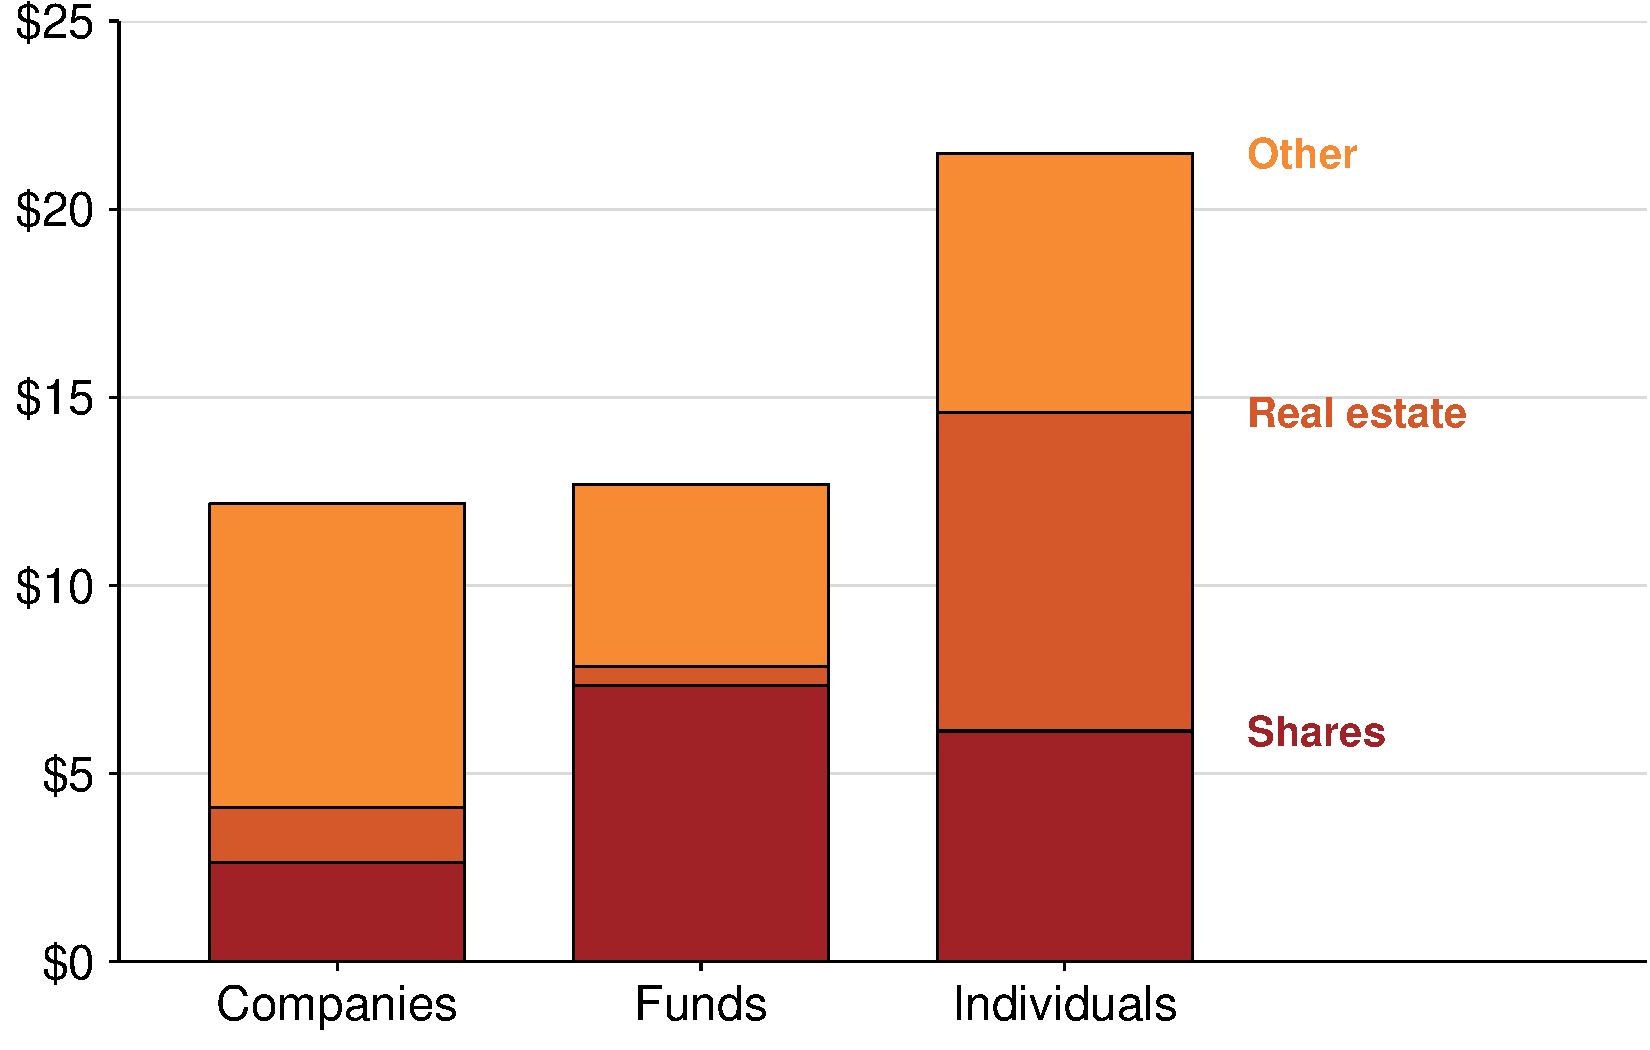
\includegraphics[width=\columnwidth]{figure/Majority_of_taxable_gains_are_earned_by_individuals-1}
\source{Molten combination of \textcite{ATOCapitalGainsByType}}
\end{figure}


\begin{smallbox}{A short history of capital gains tax changes}{box:short_history_CGT}
Before 1985 capital gains were untaxed in Australia. Taxes on capital gains were introduced to improve the integrity of the tax system, which was undermined by taxpayers recharacterising regular income as capital to avoid tax.\footcites{Evans2005}{Kenny2005}

Between 1985 and 1999, real capital gains (sale proceeds minus the original purchase price adjusted for inflation) were taxed at a taxpayer's marginal income tax rate. 

As recommended by the Ralph Review of Business Taxation, the Howard Government removed indexation adjustments so that tax was applied on nominal gains. To offset the removal of the indexation concession, capital gains tax was discounted by 50 per cent for individuals and 33 per cent for superannuation funds for assets held for more than a year. Capital gains of small unincorporated businesses, but not large businesses, are also discounted by 50 per cent. Small businesses also receive a range of other CGT concessions. When this regime was introduced, it was argued that it would stimulate capital markets and make the Australian regime more internationally competitive.\footcite[p.~14, 598]{BusinessTaxation1999} 

The tax concession is a crude way to adjust for the effects of inflation. It results in a lower tax bill compared to taxing real gains so long as asset values grow at least twice the rate of inflation. Given the strong real growth in asset prices, particularly residential property, since the discount was introduced governments have almost certainly lost revenue from the change.

\end{smallbox}
Before 1985, capital gains were not taxed in Australia. Since then, the tax treatment of capital gains has varied, but they are taxed at a lower rate than wage and salary income (\Vref{box:short_history_CGT}).  

Under the current rules, net capital gains are included as part of assessable income.\footnote{Capital losses can only be offset against capital gains, not ordinary income. But if taxpayers are unable to utilise their capital losses is a particular year, they are carried forward to future years \textcite{ATO2014a}.}  For individuals and small businesses, 50 per cent of their capital gains are excluded from income if they hold the asset for more than one year. This means the effective tax rate paid on these gains is half the rate for other forms of income. For superannuation funds, a third of their gains are excluded. Large corporations pay tax on all of their capital gains at the corporate tax rate of 30 per cent.

Capital gains have other less explicit tax advantages compared to recurrent income. Investors control when they realise gains. Consequently, they can reduce their tax by selling assets when their income is low, such as after retirement, so they are taxed at a lower marginal rate.\footnote{A common strategy for investors close to retirement is to shift capital assets into Self Managed Super Funds, and then sell them when they are aged over 60 and not liable for tax.}  For example, \textcite{Wood2010a} found that after adjusting for other factors, the probability of a landlord selling a property increases by over 20 percentage points once they retire.\footnote{The Age Pension asset test also encourages those moving into retirement to sell their assets. \textcite{Wood2010a}.}
Further, unlike other forms of income, capital gains are taxed on sale rather than as they accrue. This deferral of tax is akin to the government providing the investor with an interest free loan. (See \Vref{sec:ShouldCapitalGainsBeTaxedConsistently})

\section{Should capital gains be taxed consistently with other forms of income?}\label{sec:ShouldCapitalGainsBeTaxedConsistently}
Capital gains and other forms of savings income increase a person's spending power. It is arguable that all increases in spending power should be taxed consistently regardless of how they are earned (chapter 2)  or as the Canadian Carter report puts it ``a buck is a buck is a buck.''  But in practice, many forms of income from investments -- including owner occupied homes,  superannuation  and capital gains -- are taxed less than income from working. 

Taxing capital gains consistently with other forms of income would reduce the incentive for speculative investments and revenue leakage from artificially structured transactions. It is also highly progressive because most capital gains income is earned by the wealthy. 

On the other hand, capital gains are not the same as other forms of income. There is genuine concern that increasing taxes on capital gains might reduce incentives to save and start new businesses. But personal income tax rates are not the most important determinants of these decisions. While capital gains are eroded by inflation, so are all forms of investment returns. This does not provide a rationale for special treatment of gains. 

The most compelling reason for taxing capital gains at a lower rate is to moderate the effect of `asset lock in', whereby investors are deterred from selling assets that have accrued large gains. This could be more directly dealt with through moving to a system where gains are taxed on an accrual basis.  

\subsection{Tax concessions for capital gains generate revenue leakage and favour the wealthy}
A lower tax rate for capital gains results in `revenue leakage' as taxpayers find ways to convert income into capital gains.\footcites{Evans2005}{Minas2013}  Protecting the income tax base is a key reason capital gains are taxed in most OECD countries.\footcite{OECD2006b}

Tax concessions for capital gains favour wealthy taxpayers who receive most of the capital gains. Almost 80 per cent of capital gains are earned by those in the top 20 per cent of income earners (\Vref{fig:Nearly_eighty_per_cent_of_capital_gains_are_earned_by_those_}). Compared to low income earners, higher income earners are more likely to have additional income that can be invested.\footnote{The top 20 per cent of households by disposable income save on average 35 per cent of their disposable income. This compares to dissavings of 25 per cent for the lowest income quintile and savings rates of less than 10 per cent for the second and third quintiles.}


\begin{figure}
\Caption{Nearly eighty per cent of capital gains are earned by those in the highest income quintile}{Amount of net capital gains by income decile}{fig:Nearly_eighty_per_cent_of_capital_gains_are_earned_by_those_}
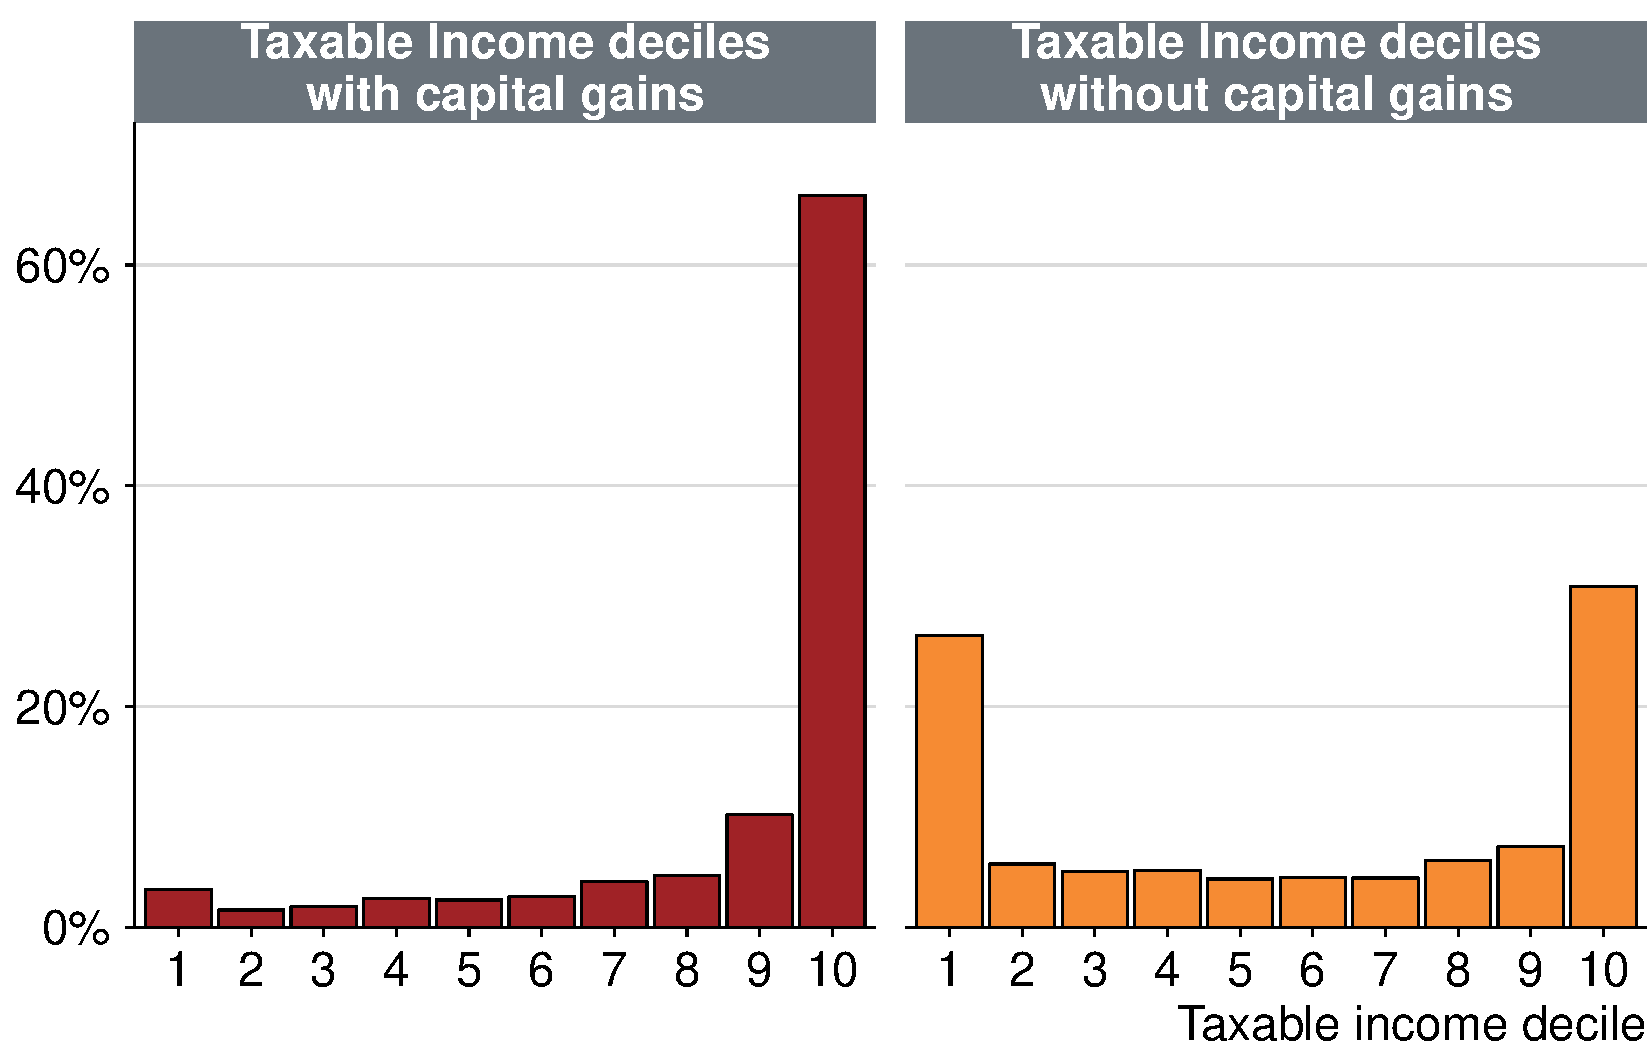
\includegraphics[width=\columnwidth]{figure/Nearly_eighty_per_cent_of_capital_gains_are_earned_by_those_-1}
\source{\gao\ \textcite{ATO2013i}}
\end{figure}
\subsection{Adjusting for inflation is not consistent with treatment of other forms of income}
A lower tax rate for capital gains is sometimes justified on the basis that the effective tax rates on real returns can be high if nominal gains are taxed at marginal income tax rates.\footcite{Treasury2010} This is particularly true of investments with low real returns that are held for an extended period (\Vref{box:short_history_CGT}).

In our system, labour and investment income are taxed in nominal terms.\footcite{Treasury2010}  And income tax deductions, such as interest payments for investment property are also deducted on a nominal basis (section 

Periodic adjustments are made to the income tax thresholds to compensate for inflation and wages growth. While imperfect, these adjustments help mitigate the effects of inflation on effective tax rates for income, including capital gains.

Making additional inflation adjustments for capital gains magnifies the tax advantages capital gains receive over other investment income. Ironically Australia's current system provides no adjustments for the least protection to bank deposits -- disproportionately held by the least well off -- and much more protection for other investments.

Unlike other investment income, gains are taxed when an asset is sold, not when they accrue, which provides investors with an implicit interest-free loan on tax liabilities (\Vref{box:Tax_deferral_and_effective_tax_rates}).\footcites[See also:][p.~2]{Fane2004}[p.~12]{Ingles2009} Investors are also able to choose the time of the asset's disposal to minimise tax. 

\afterpage{%
\begin{bigbox*}{Tax deferral and effective tax rates}{box:Tax_deferral_and_effective_tax_rates}
Even without a discount, capital gains are taxed at a lower effective rate than other forms of investment income such as interest or dividends because the tax can be deferred until the asset is sold. 

Suppose a person has \$100,000 to invest over ten years. They can choose either a bank term deposit that earns 6 per cent interest a year or a property that does not generate any recurrent income (rental payments just cover the annual expenses) but is expected to appreciate in value at 6 per cent a year. The investor is in the second top tax bracket and pays 37 per cent tax on income. For simplicity, we assume no adjustments are made to the tax rates or thresholds to correct for the effects of inflation.

If the investor chooses the term deposit, they reinvest the after-tax income each year.  After ten years, the amount in the term deposit would be \$145,000. Real after-tax returns are 1.2 per cent per annum.  In contrast, after ten years the property would be worth \$179,000. If the property was sold at this point, there would be a taxable gain of \$79,000. If capital gains were taxed at the investor's full marginal rate of 37 per cent, the investment would be worth \$150,000, a real after tax return of 1.6 per cent per annum. (With the 50 per cent capital gains tax discount the real after tax return is 2.5 per cent). 

The higher post-tax return on the property is because tax is deferred for ten years rather than paying it as it accrues. The real effective tax rate on the term deposit is 63 per cent compared to 54 per cent for the property with no capital gains tax discount.
\eject

\captionoffigurewithunits{Real effective marginal tax rates are lower for capital gains than income, especially after the capital gains tax discount}{Real effective marginal tax rate}\label{fig:Real_effective_marginal_tax_rates_are_lower}
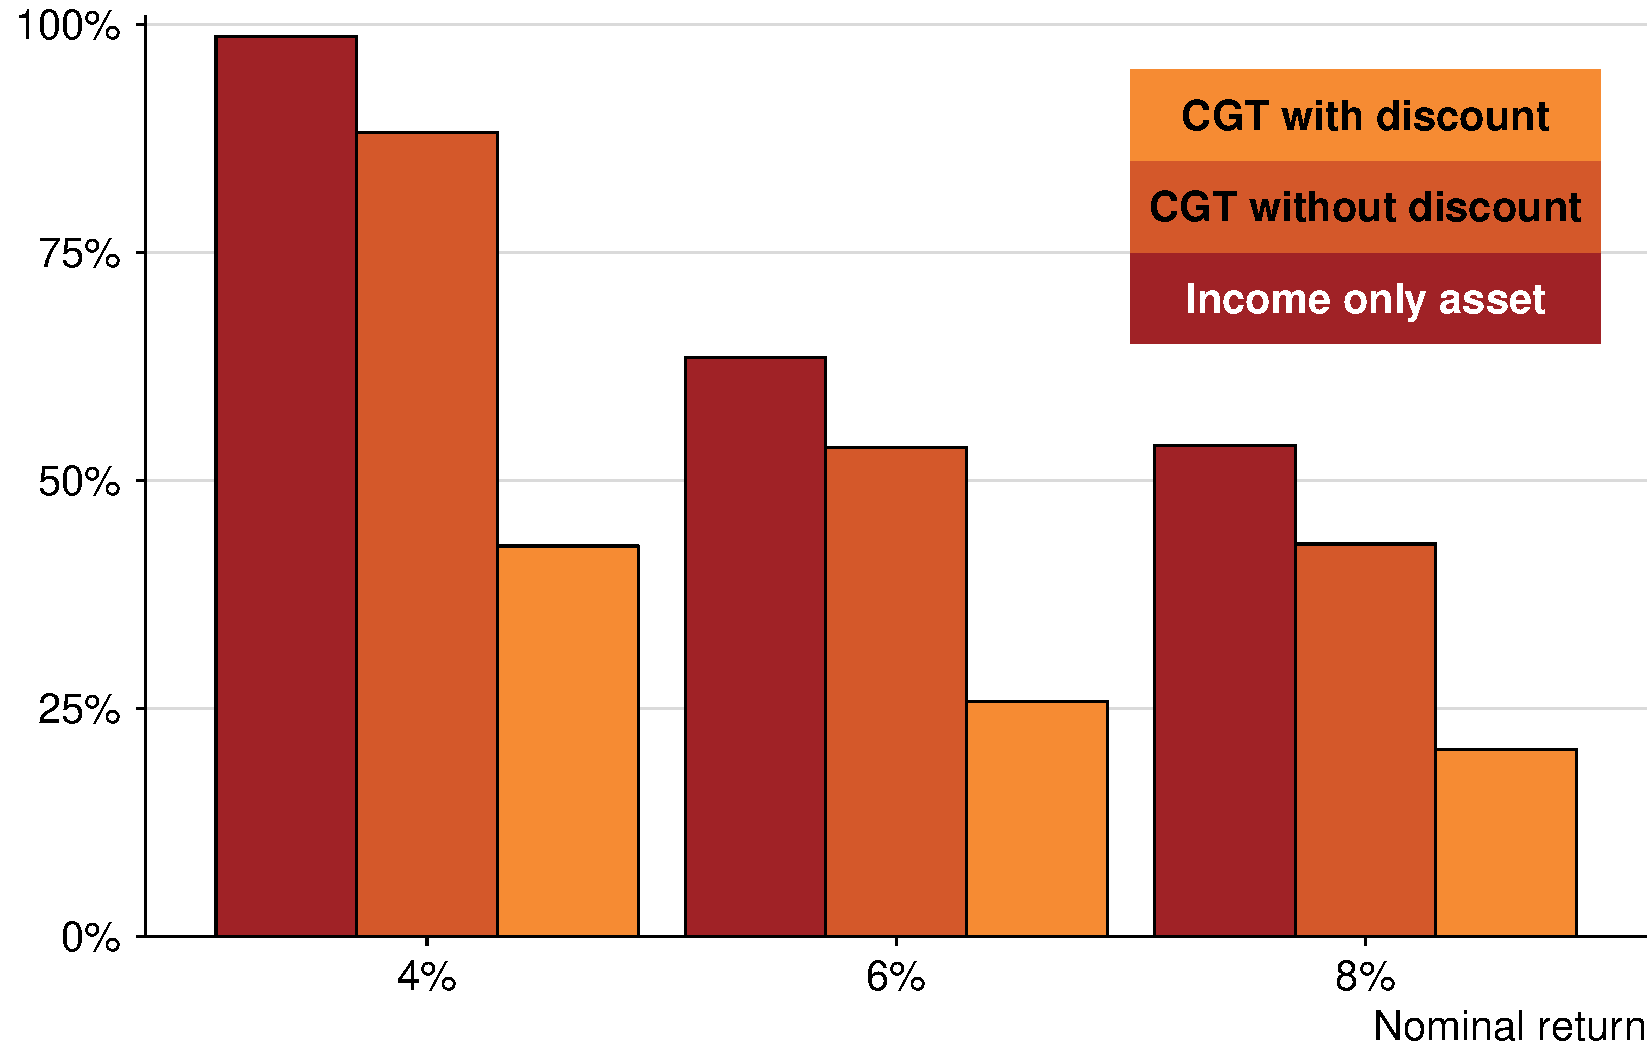
\includegraphics[width=\columnwidth]{figure/Real_effective_marginal_tax_rates_are_lower-1}
\notes{Income only asset is a bank account or bond that generates income but has no capital growth. Growth asset is asset that generates all returns through capital gain. Assumptions: inflation is 2.5 per cent, the person pays all tax on investment income at the marginal tax rate of 37 per cent and assets are held for ten years.}

\source{Grattan analysis}
\end{bigbox*}
}



\subsection{Taxing capital gains without a discount will not substantially distort economic decisions}
Taxing capital gains at the full marginal rate could deter entrepreneurship and risk taking by reducing the returns to selling a successful business.\footnote{If capital gains were taxed on an accrual basis and capital losses were fully deductible against all assets, then taxing gains in full would be neutral with respect to risk. However, since losses are only deductible against gains this increases the risk that investors will make a loss they are not able to deduct. It is not clear whether deferral of taxes on gains until realisation, itself a significant tax advantage (section x.1), is itself enough to compensate investors for this risk. \textcite[p.~8]{Burman2009};  \textcite[p.~130]{Commission2004}}  But this effect may not be large. There are other factors that drive entrepreneurship and risk taking behaviour that are far more significant than the tax on any gains ultimately made.\footcite[p.~75]{Burman1999}   Further, other exceptions already in place limit the effects of capital gains tax when assets or businesses are sold.\footnote{Capital gains tax exemptions are available for the sale of active assets by small business up to a lifetime limit of \$500,000 provided the gains are paid into a complying super fund. There are also exemptions for people over 55 that are retiring and selling business asset held for more than 15 years. Small business also receive rollover relief allowing them to defer all or part of a capital gain for two years or longer on the sale of active assets, provided they acquire a replacement asset or you incur expenditure on making capital improvements to an existing asset. \textcite{ATO2014e}}

In any case, capital gains tax concessions \emph{for individuals} are a very inefficient way to stimulate investments in new enterprises. While individuals provide almost all of the human capital for new ventures, much of the financial capital invested in new firms comes from institutional investors, foreigners or corporations that do not receive the capital gains tax discount.\footcite{Burman1999}  Meanwhile, individuals that get the discount mainly claim it for investments in shares and real estate (\Vref{fig:Majority_of_taxable_gains_are_earned_by_individuals}). 

Taxing capital gains at the full marginal rate might also reduce savings but the effects are unlikely to be large. Taxes on capital gains, as for other taxes on savings income, create a bias against savings towards current consumption (chapter 2).  But empirical evidence suggests that savings may not be particularly responsive to tax rates, particularly for high income earners. For example, \textcite{Engen1996} finds that tax breaks for saving influence the choice of savings vehicle but do not increase overall household savings much. And the OECD finds that tax breaks for saving are generally ineffective for high income earners because this group are likely to save anyway.\footcite{OECD2007}  \textcite{chetty2013subsidies} show that reduced subsidies for retirement savings for high income earners lead to almost no reduction in overall savings efforts.\footnote{\textcite{chetty2013subsidies} ) is a particularly compelling study because of the strength of the data (41 million observations on savings for people from Denmark). But it is also consistent with the thrust of the literature on the effect of tax incentives for retirement savings. While findings vary across studies, a summary by \textcite{Antolin} suggests tax incentives increase savings mostly by reallocation from other savings vehicles. }

The other economic cost of higher taxes on capital gains is greater asset lock in. 

Because taxes are only paid when gains are realised, investors are encouraged to hold on to assets with large accumulated gains.\footcite[p.~69]{Burman2009} In effect, the investor seeks to maintain the implicit interest free loan on accrued gains. Crystallising a capital gain is only worthwhile if an investor can achieve a materially higher return (\Cref{box:CGT_asset_lockin}).\footcite[p.~12]{Ingles2009} 

\begin{smallbox}{Capital gains tax and asset lock in}{box:CGT_asset_lockin}
Suppose Hayley, an investor in the top tax bracket purchases a house for \$700,000 and holds it for 10 years. During that time the market price of the house increases to \$1 million. She makes a net rental return of 5 per cent a year, giving her a \$50,000 income stream. 

If she were to sell the house she would crystallise the \$300,000 in gains, paying tax on 50 per cent of the gains at her marginal tax rate of 49 per cent (\$73,500). This would leave her with around \$926,500 from the sale: \$226,500 in net gains and her initial investment of \$700,000. In order to better her income of \$50,000 and make the sale worthwhile, she needs to find an investment (with the same opportunity for capital gains) that pays net returns of more than 5.4 per cent a year.

If capital gains were taxed in full, rather than at the current 50 per cent discount, her hurdle rate for the new investment would be 5.9 per cent. 
\end{smallbox}

Lock-in is a problem because it discourages investors from moving their money to the investments with the highest pre-tax returns, and it discourages sale of assets to those who can increase the returns achieved by the current owner.\footcite{Lindsey1987}  Lock-in effects are most significant from a whole of economy perspective, if they constrain financing of profitable investments.\footcites{OECD2006b}{Johnson2008}  Australia's open capital markets and generous capital gains tax regime for non-residents reduce the danger that worthwhile projects will not get access to capital because of lock-in.\footnote{Non-resident investors in Australian shares are generally not subject to Australian capital gains tax. See \Act{Income Tax Assessment Act 1936}{Cth}~s.136-25.}  

Ultimately, the best way to reduce asset lock-in is to tax gains on an accruals basis, with interest charges on the deferred tax.\footcite[pp.~11-14]{Burman2009} This would remove the incentive to hold on to gains to reduce the tax burden. 

To date, annual asset revaluations have been considered impractical and beset with administrative difficulties.\footcites{OECD2006a}{Commission2004} But such valuations can be done easily for shares and to a lesser extent property (which is already revalued in most states every one or two years for the purposes of levying council rates (chapter 5)).\footcites{Burman2009}[p.~12]{Ingles2009} The Henry review flagged that such an accruals approach to capital gains becomes more feasible as technology improves.\footcite[p.~64]{Treasury2010} 

Most OECD countries offer some type of discount or concession for capital gains but it varies by investment type.\footnote{In some countries -- including Israel, Ireland, Norway, and Luxembourg -- property investments other than the family home are taxed as ordinary income. See \textcite{Harding2013} for a summary.}  But the hurdles to qualify for the most generous concessions can be stringent. Holding periods to receive maximum concession on investment property are ten years in Germany and Korea, 20 years in Slovenia, 30 years in France and 35 in Austria.\footcite{Harding2013} In New Zealand, where capital gains are notionally tax free, capital gains on property purchased with the intent to sell is taxed as ordinary income.\footcite[p.~25]{prebble2010tax} 

\section{Negative gearing benefit provides generous tax treatment for investors}\label{sec:negative_gearing_provides}
Negative gearing allows taxpayers to subtract the losses they make on investments (including mortgage interest payments) from their taxable income including wages. 

The ability to offset losses against other income is part of the normal operation of the Australian tax system, and applies to a wide range of investments and business activities. If losses were not deductible, they would be treated asymmetrically to gains (which are taxed) and investments in risky assets would be less attractive. Deductibility of interest payments in theory maintains tax neutrality for investors choosing between lending and equity financing.\footcite{Fane2004}  


But the issue for negatively geared property or shares is that the loss being deducted is illusory. Investors are only willing to make an income loss over a number of years because the value of the asset is growing. But the gains in property value are not counted as income until the asset is sold (section 1.2). It is the combination of unlimited deductions of "losses" against wage income while only being taxed on half the gains upon realisation that makes negative gearing an attractive strategy.\footcite[pages~5,13]{ACOSS} 

This comes at both a cost to the budget and potentially negative impacts in investment markets, particularly housing markets, where the tax treatment has encouraged speculative activity. 

\subsection{Negative gearing is growing in popularity, mainly for housing investment}
There has been a boom in negatively geared residential property investments over the last two decades. Other than a temporary dip following the global financial crisis, both the number of taxpayers making losses on residential property investment and the average loss made has increased steadily (\Vref{fig:Negative_gearing_real_over_time})




\begin{figure}[t]
\Caption{The introduction of the capital gains discount, but not the introduction of negative gearing, led a large fall in rental profits.}{Total net rent, billions (2013-14~dollars)}{fig:Net_rent_over_time}
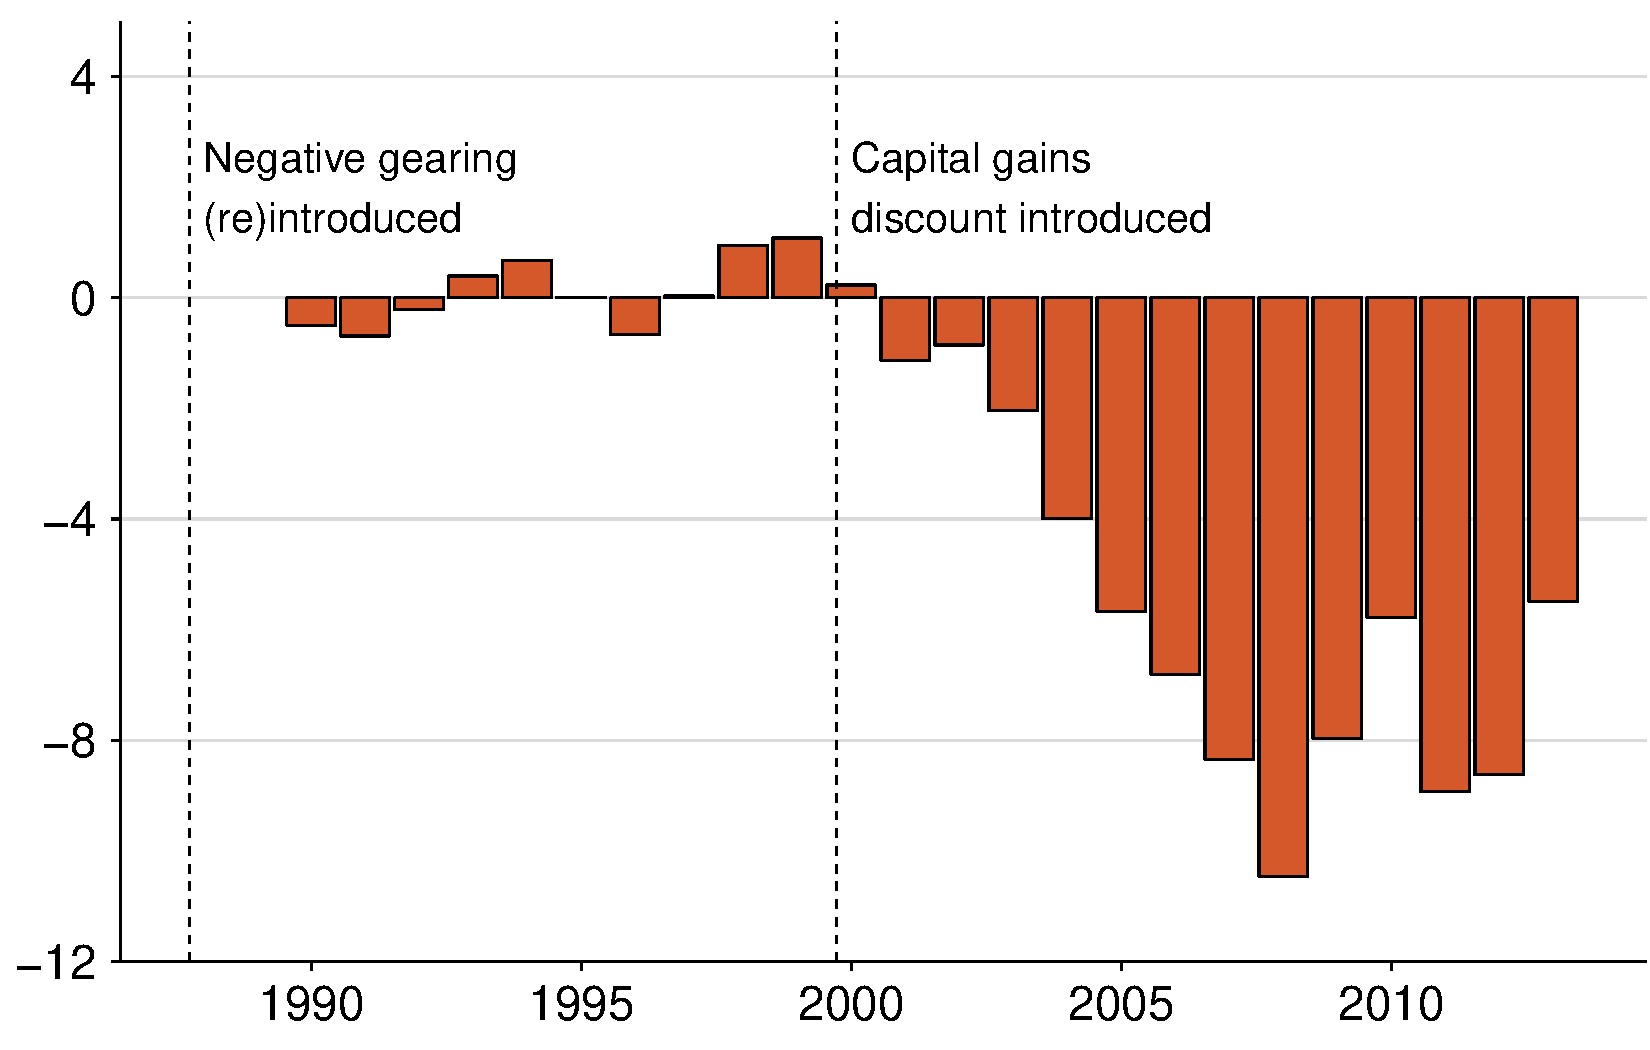
\includegraphics[width=\columnwidth]{figure/Net_rent_over_time-1}
\notes{Net rent as marked by taxpayer upon lodgement of tax return}

\source{ATO taxstats 1979-2013 (data not available pre-1989)}
\end{figure}

\begin{knitrout}
\definecolor{shadecolor}{rgb}{0.969, 0.969, 0.969}\color{fgcolor}\begin{kframe}
\begin{verbatim}
## Response [http://data.gov.au/dataset/e29ef9ca-0d1a-47ec-9e9b-14a79a941511/resource/5bfb5001-2d3c-46cb-a76d-1b86b6913ac3/download/taxstats2013company1selecteditemsforincomeyears197980to201213.xlsx]
##   Date: 2015-06-22 15:49
##   Status: 200
##   Content-Type: application/vnd.openxmlformats-officedocument.spreadsheetml.sheet
##   Size: 116 kB
## <ON DISK>  taxcompanies_time_series1979-2013.xlsx
\end{verbatim}
\end{kframe}
\end{knitrout}


\begin{figure}[t]
\Caption{Did companies divest of assets yielding negative returns for individuals to lap up, after the discount was introduced}{Net rent (companies), \$~billions, (2013-14 dollars)}{fig:Net_rent_over_time_companies}
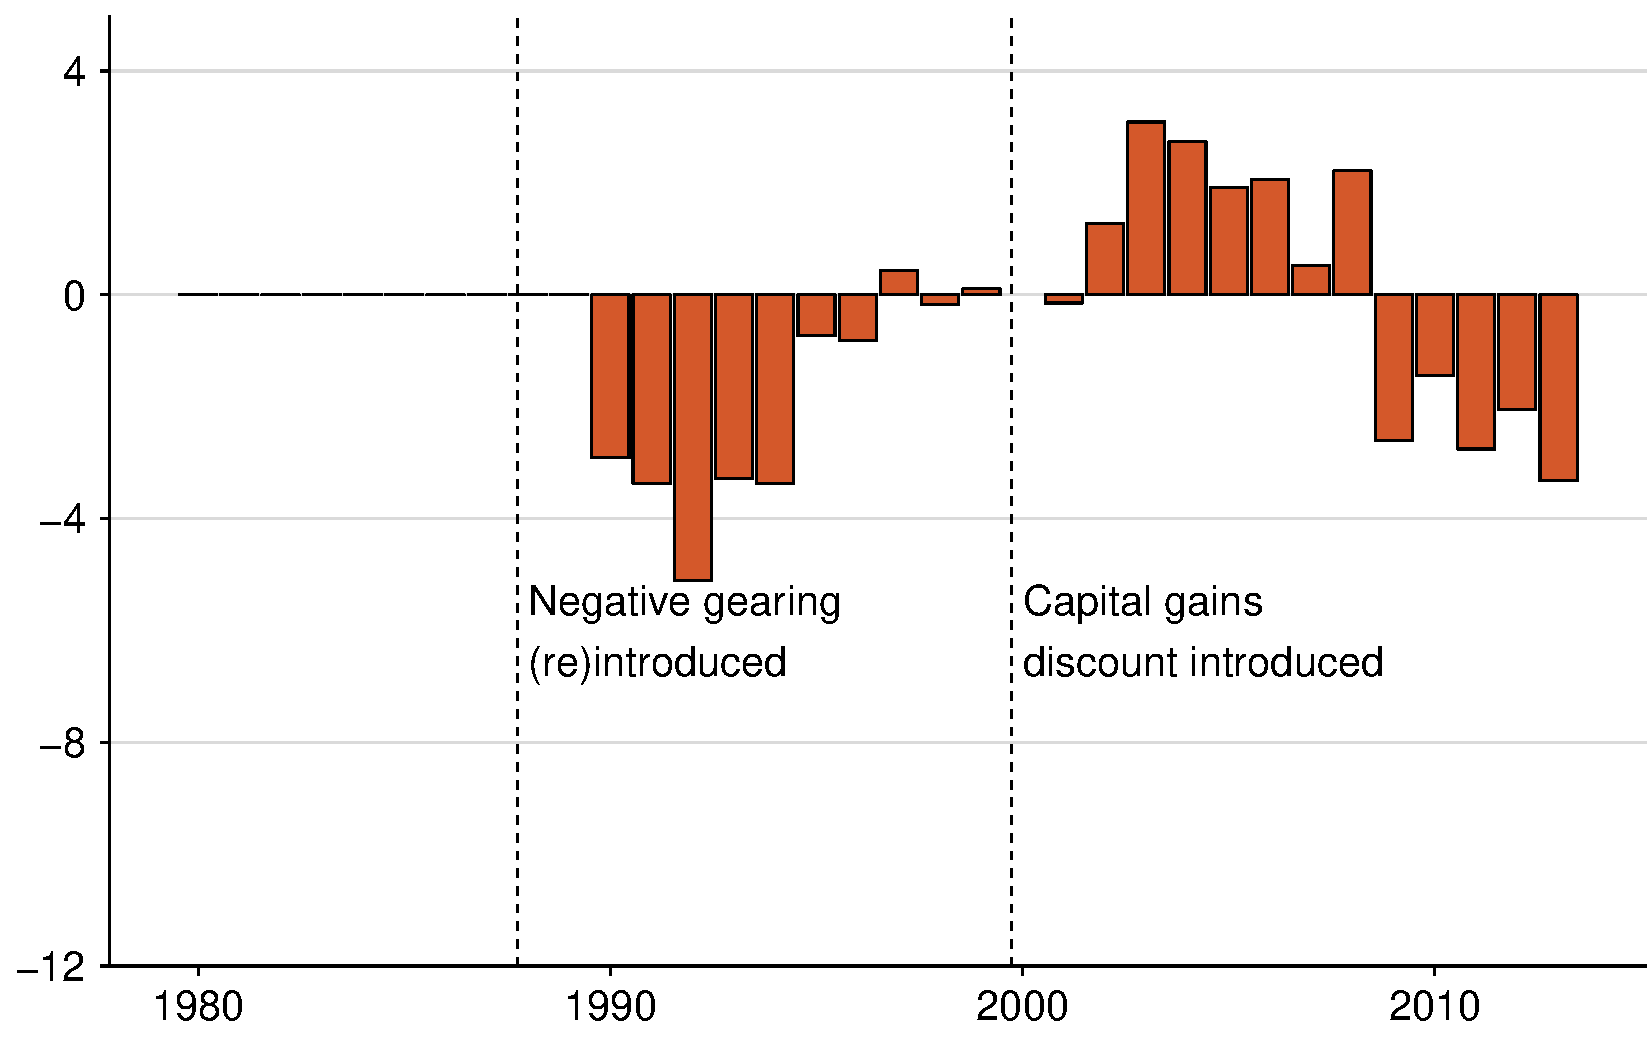
\includegraphics[width=\columnwidth]{figure/Net_rent_over_time_companies-1}
\source{Simple calculation of \url{http://data.gov.au/dataset/e29ef9ca-0d1a-47ec-9e9b-14a79a941511/resource/5bfb5001-2d3c-46cb-a76d-1b86b6913ac3/download/taxstats2013company1selecteditemsforincomeyears197980to201213.xlsx}}
\end{figure}



\begin{figure}
\Caption{More people are negatively gearing and the losses are growing even faster}{Number of people negatively gearing and real amount negatively geared (in 2012-13 dollars). First year = 1.}{fig:Negative_gearing_real_over_time}
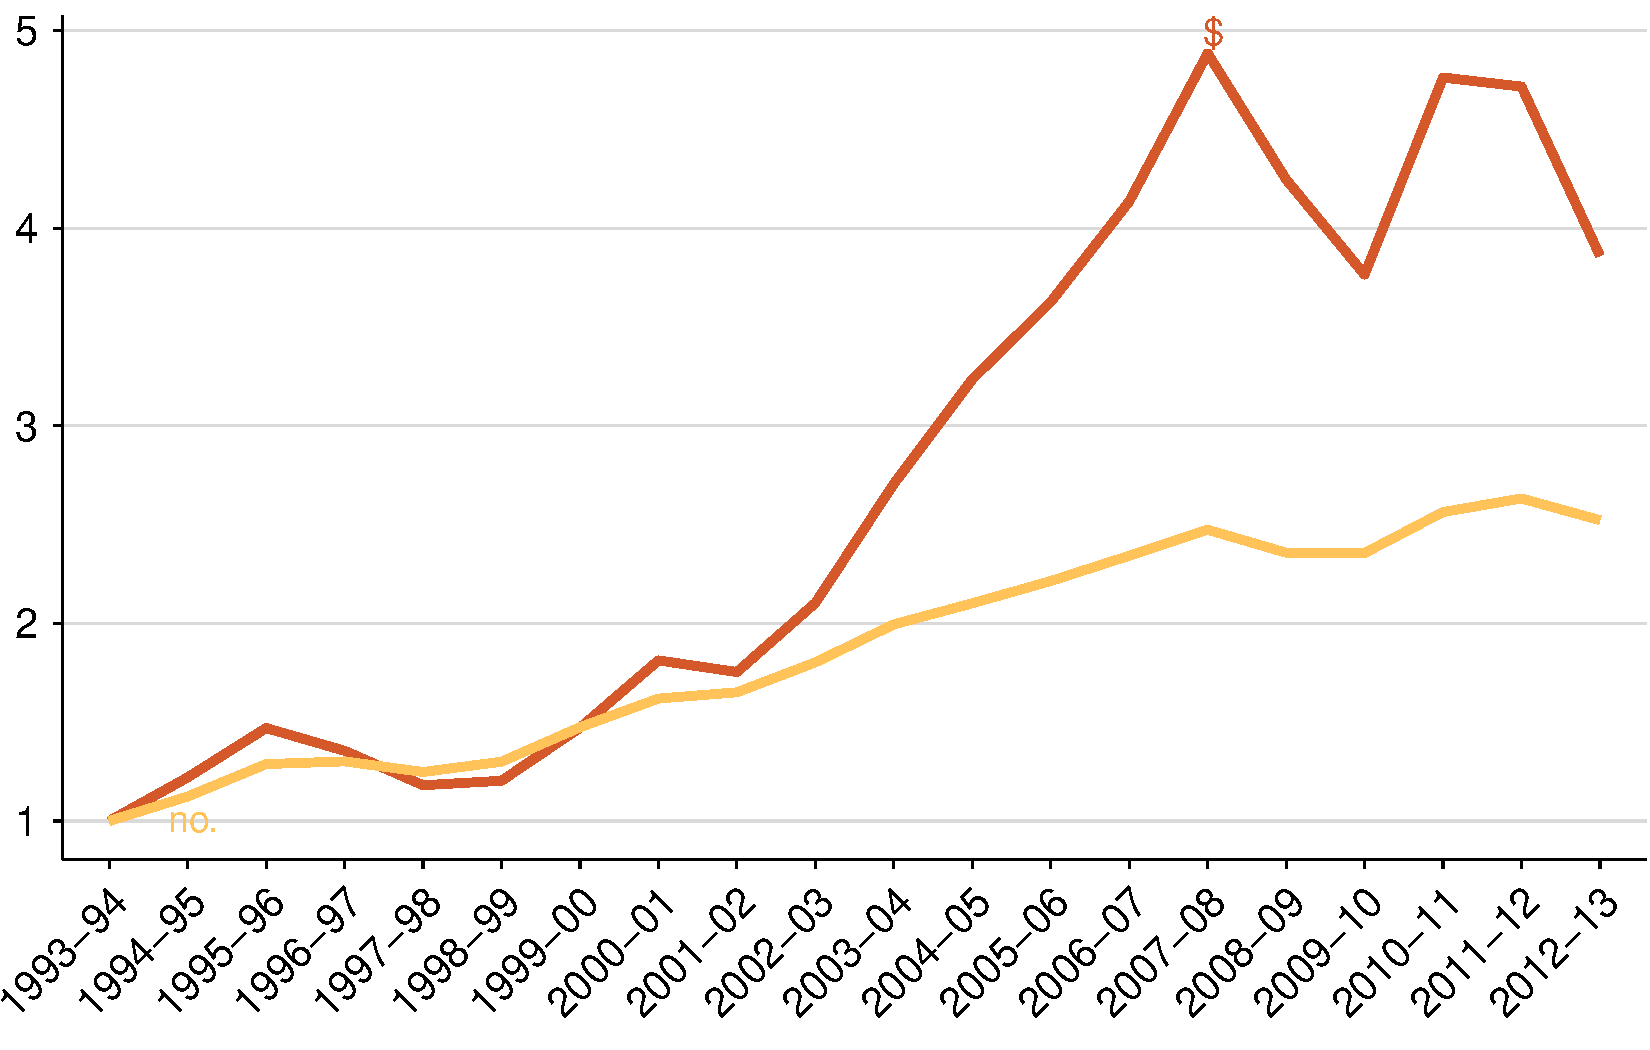
\includegraphics[width=\columnwidth]{figure/Negative_gearing_real_over_time-1}
\notes{Amount deflated by CPI. Other indices may be more useful.}

\source{\gao\ \url{https://data.gov.au/dataset/e29ef9ca-0d1a-47ec-9e9b-14a79a941511/resource/233cbf28-6fda-4e53-bbe9-3a37a65fb742/download/taxstats2013individual01selecteditemsbyyear.xlsx}}
\end{figure}
The average property investor is making a loss of more than \$5000 annually. The majority of the loss is mortgage interest payments. (\Vref{fig:Interest_makes_up_the_bulk_of_rental_deductions})


\begin{figure}
\Caption{Interest makes up the bulk of rental deductions}{Rent and deductions for residential property investors, billions of dollars (2012-13)}{fig:Interest_makes_up_the_bulk_of_rental_deductions}
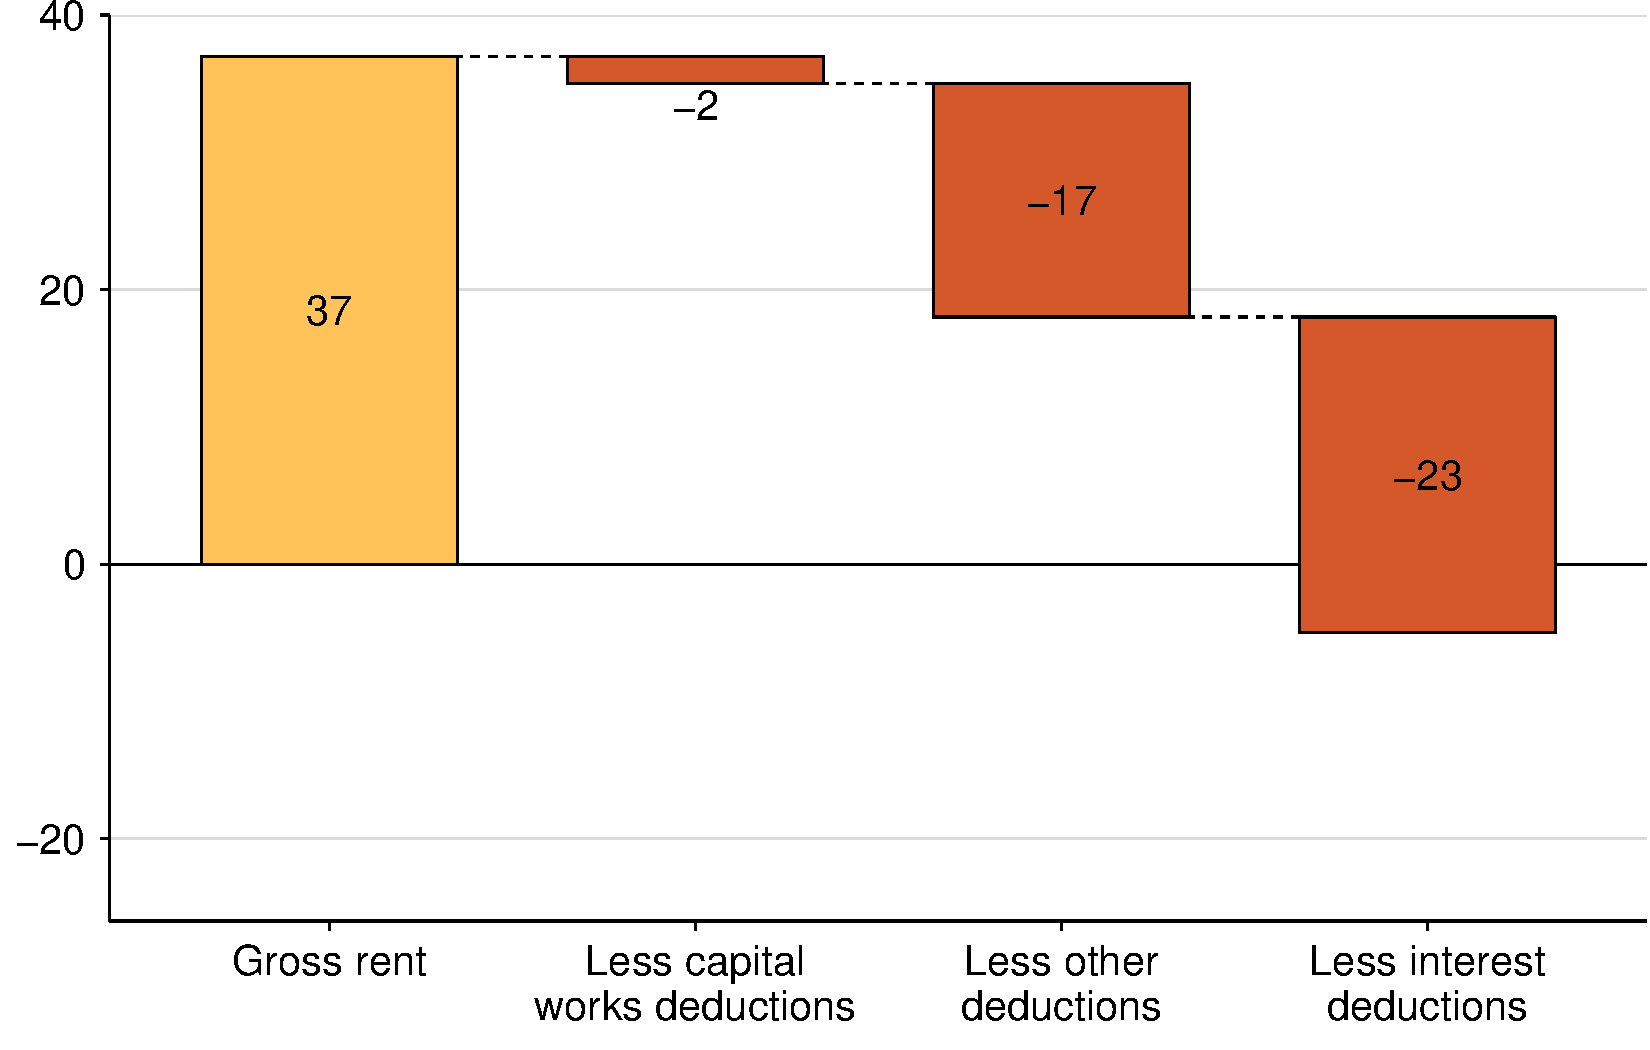
\includegraphics[width=\columnwidth]{figure/Interest_makes_up_the_bulk_of_rental_deductions-1}
\notes{}

\source{Grattan analysis of \textcite{ATO2013i}.}
\end{figure}

Negative gearing is used much less for investments outside of housing. Even at the height of the share market boom, only about 10 per cent of investments outside of superannuation were funded by borrowing -- and many of them were positively geared;\footcite{Daley2007}  since then margin lending has reduced by around 70 per cent from its peak in 2007.\footcite{RBA2015a}
\subsection{Interaction with capital gains tax discount encourages leveraged and speculative investment activity}
Taxes on capital gains are discounted by 50 per cent and only paid when the asset is sold. But negative gearing arrangements allows investors to deduct ``losses'' -- investment expenses  (including interest costs) in excess of rental income from wage income that would otherwise be taxed at the full marginal rate.\footnote{In reality, the assets are generally not making a loss because they accruing a capital gain. It is simply that this gain is not taxed until realisation. See: \textcite{ACOSS}[pp.~12-13.]}

This makes it more attractive to invest in assets that offer low returns on the expectation of future capital growth. This has played a role in investors being prepared to accept rental yields that are lower than those seen in other countries. As \textcite[p.~42]{RBA2014} notes:

\begin{quote}
\dots in most countries the earning of rental income is seen as the most important reason for investing in rental properties. \dots\ This seems to stand in contrast to the situation in Australia where properties are commonly marketed on the presumption that they do not earn positive taxable income for a considerable period.
\end{quote}

The asymmetry between the tax treatment of gains and losses also makes debt financing of investment more attractive. The Henry tax review estimated that for a high income taxpayer investing in a rental property, effective marginal tax rates are negative for a 70 per cent geared property, but almost 50 per cent if the property is owned outright.\footnote{For a tax payer on 46.5 per cent marginal rate (the top tax rate at the time), 6 per cent nominal return, 2.5 per cent inflation, 50 per cent return attributed to capital gains and 50 per cent to rental income. Rental property held for 7~years. \textcite[p.~74]{Treasury2010}}  It described the asymmetry between gains and losses as ``among the greatest tax induced biases to the savings choices of households''.\footcite[p.~69]{Treasury2010}  This runs contrary to the rationale for allowing the deductibility of losses -- to maintain tax neutrality of debt and equity financing. 

Borrowing to finance an investment with low yields but high potential capital appreciation allows an investor to reduce and defer their tax by effectively converting salary income into capital gains. 

The effect is to incentivise leveraged and speculative investments, particularly for property.\footcite[p.~17]{Inquiry2014} Investors have responded to these incentives. Before the capital gains tax discount was introduced in 1999, there were 1.3 million landlords making an aggregate taxable profit of \$0.7~billion. By 2012-13, there were 2 million landlords making collective losses of \$5.5 billion.\footcites{Eslake2013}{ATO2015} Over this same period, the proportion of property investors making losses on their investment increased from around 50 per cent to 65 per cent.\footcite{ATO2014e} 

The average level of gearing for property investors is increasing. Even though interest rates are falling, interest deductions as a proportion of rents increased from 45.6 per cent of gross rental payments in 1997-98 to 71.1 per cent in 2011-12.\footcite[p.~65]{Treasury2015}

The favourable tax treatment for investors drives up house prices because it increases the after-tax returns to housing investors.\footnote{FOr example, \textcite{Commission2004} found that these tax settings had added to the housing price boom by encouraging investors to reduce current income in favour of longer term gains.} This helps existing home-owners but accelerates falling rates of home ownership among younger age groups.

\subsection{Reducing tax on wage income is particularly attractive}
Using negative gearing to reduce and defer tax is a particularly attractive strategy for those with high wage incomes. Of course, negative gearing only makes sense if the expected capital gains (and any positive income) exceed the income losses over the time the asset is held. But for some investors, reducing taxes on their wages has become one of the primary goals. Investment advisors frequently warn investors against placing too much emphasis on tax breaks and not enough on the financial returns to the investment.\footcite[See for example:]{Brown2012}

The attractiveness of using investment losses to reduce taxes on wage income is evident in the age profile of those negatively gearing property. (\Vref{fig:Age_negative_gearing_investments}) Investing in loss making properties is popular amongst those of working age, but far less prevalent amongst over 60s who are unlikely to benefit from the tax write-offs. Over 60 per cent of those under 60 with investment properties make rental losses compared to less than 40 per cent over 60. 


\begin{figure}
\Caption{More people negatively gear investments in their peak earning years}{Negative gearing status, percentage within each age group.}{fig:Age_negative_gearing_investments}
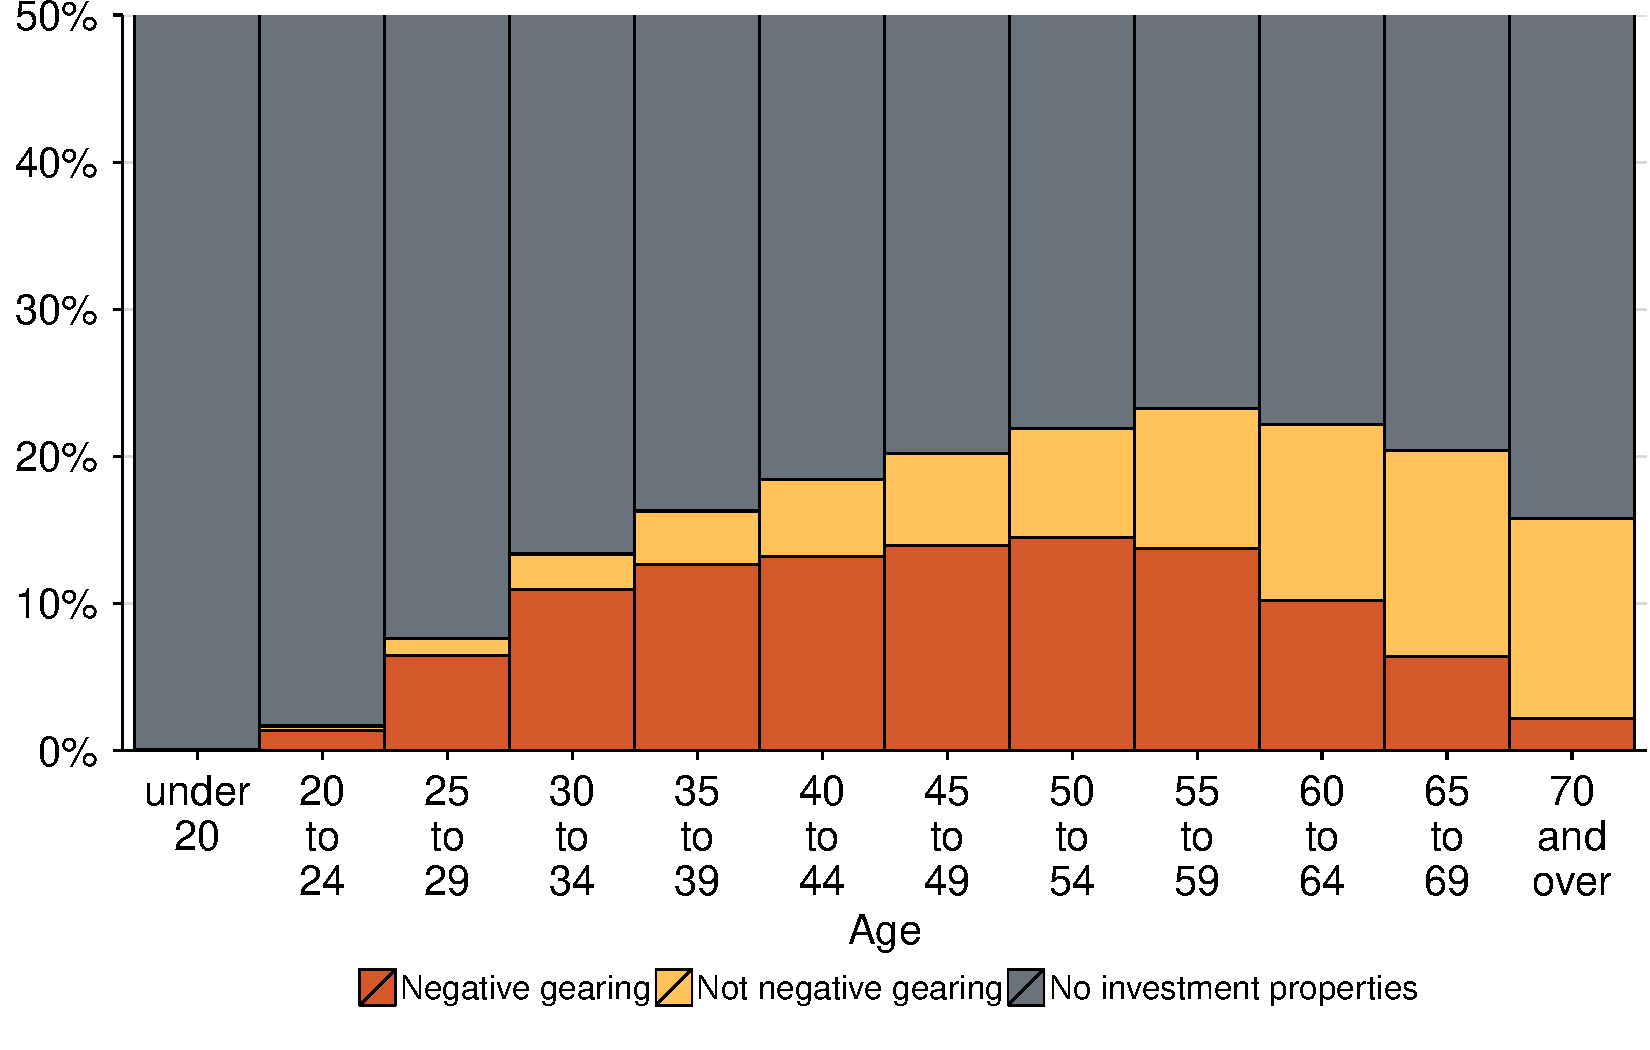
\includegraphics[width=\columnwidth]{figure/Age_negative_gearing_investments-1}
\notes{The top 50\%\ of the chart is not shown -- it would be grey all the way to 100\%. ``No investment properties'' means gross rental income is zero.}

\source{\gao\ \textcite{ATO2013i}}
\end{figure}

Most other advanced economies provide a less generous treatment for rental losses. The Unites States only allows losses to be written off against other forms of ``passive'' income. The UK and many European countries only allow deductions against the same class of income, so for example, losses on investment property can only be used to reduce tax on income or capital gains from other investment properties. Others such as the Netherlands do not allow deductibility of losses from investment housing.\footnote{Summaries of international regimes can be found in \textcite[p.~43]{RBA2014} \textcite[p.~86]{Commission2004}, \textcite[pp.~92-95]{ODonnell2005}}% #820}. } 

\subsection{Negative gearing mainly benefits middle and high income earners}
Like most tax concessions on investment, tax benefits from negative gearing are biased to the wealthy. The increase in after-tax return as a result of the current negative gearing/capital gains interaction is larger for individuals on higher marginal tax rates, all else being equal.\footcite{Inquiry2014}   

The top 10 per cent of income earners receive more than one third of rental deductions. (See \Vref{fig:Effect_of_Deductions}.) If we look at tax deciles before rental property losses are deducted -- correcting for the fact that many better off taxpayers use rental losses to reduce their taxable income -- the top ten per cent of income earners receive almost fifty per cent of the tax benefits of negative gearing.\footnote{\textcite{RBA2015} analysis of \textcite{HILDA2015} also suggests that higher income earners are more likely to negatively gear property. It shows that the top 20 per cent of income earners are almost ten times more likely to have a debt financed investment property than those in the bottom 20 per cent of earners.} 





\begin{figure}
\Caption{Negative gearing mostly benefits those on high incomes, and the difference is especially stark when incomes are measured before subtracting rental interest deductions}{Percentage of each decile's share of the benefit in reduced income tax due to negative gearing (2012-13)}  {fig:Effect_of_Deductions}
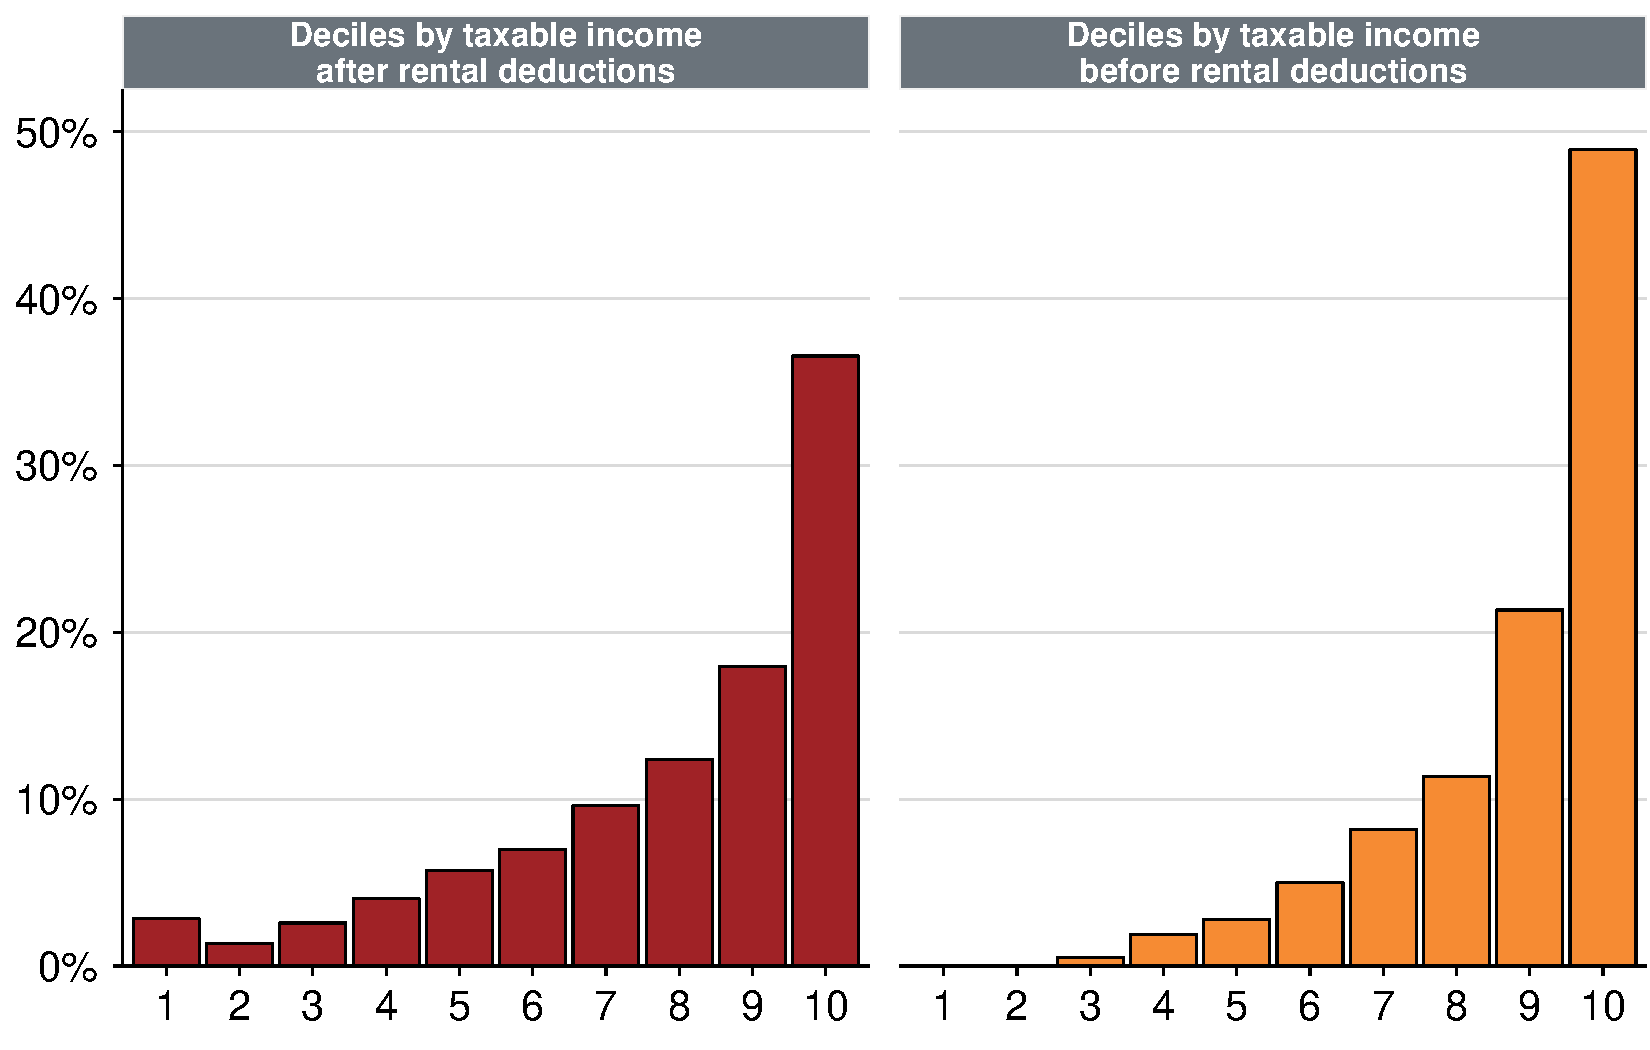
\includegraphics[width=\columnwidth]{figure/Effect_of_Deductions-1}
\notes{Taxable income before rental deductions means $\text{Taxable Income} - \min(\text{Net rental profit}, 0)$. Income tax includes medicare levy, medicare thresholds, but not other tax benefits (\emph{e.g.}~the seniors and pensioners tax offset (SAPTO))}

\source{\gao\ \textcite{ATO2013i}}
\end{figure}


% \begin{figure}
% \Caption{Negative gearing benefits mostly benefits those on high incomes, and the difference is especially stark when incomes are measured before subtracting rental interest deductions}{Average amount by which income tax was reduced due to negative gearing (2012-13)}  {fig:Effect_of_Deductions_amount}
% 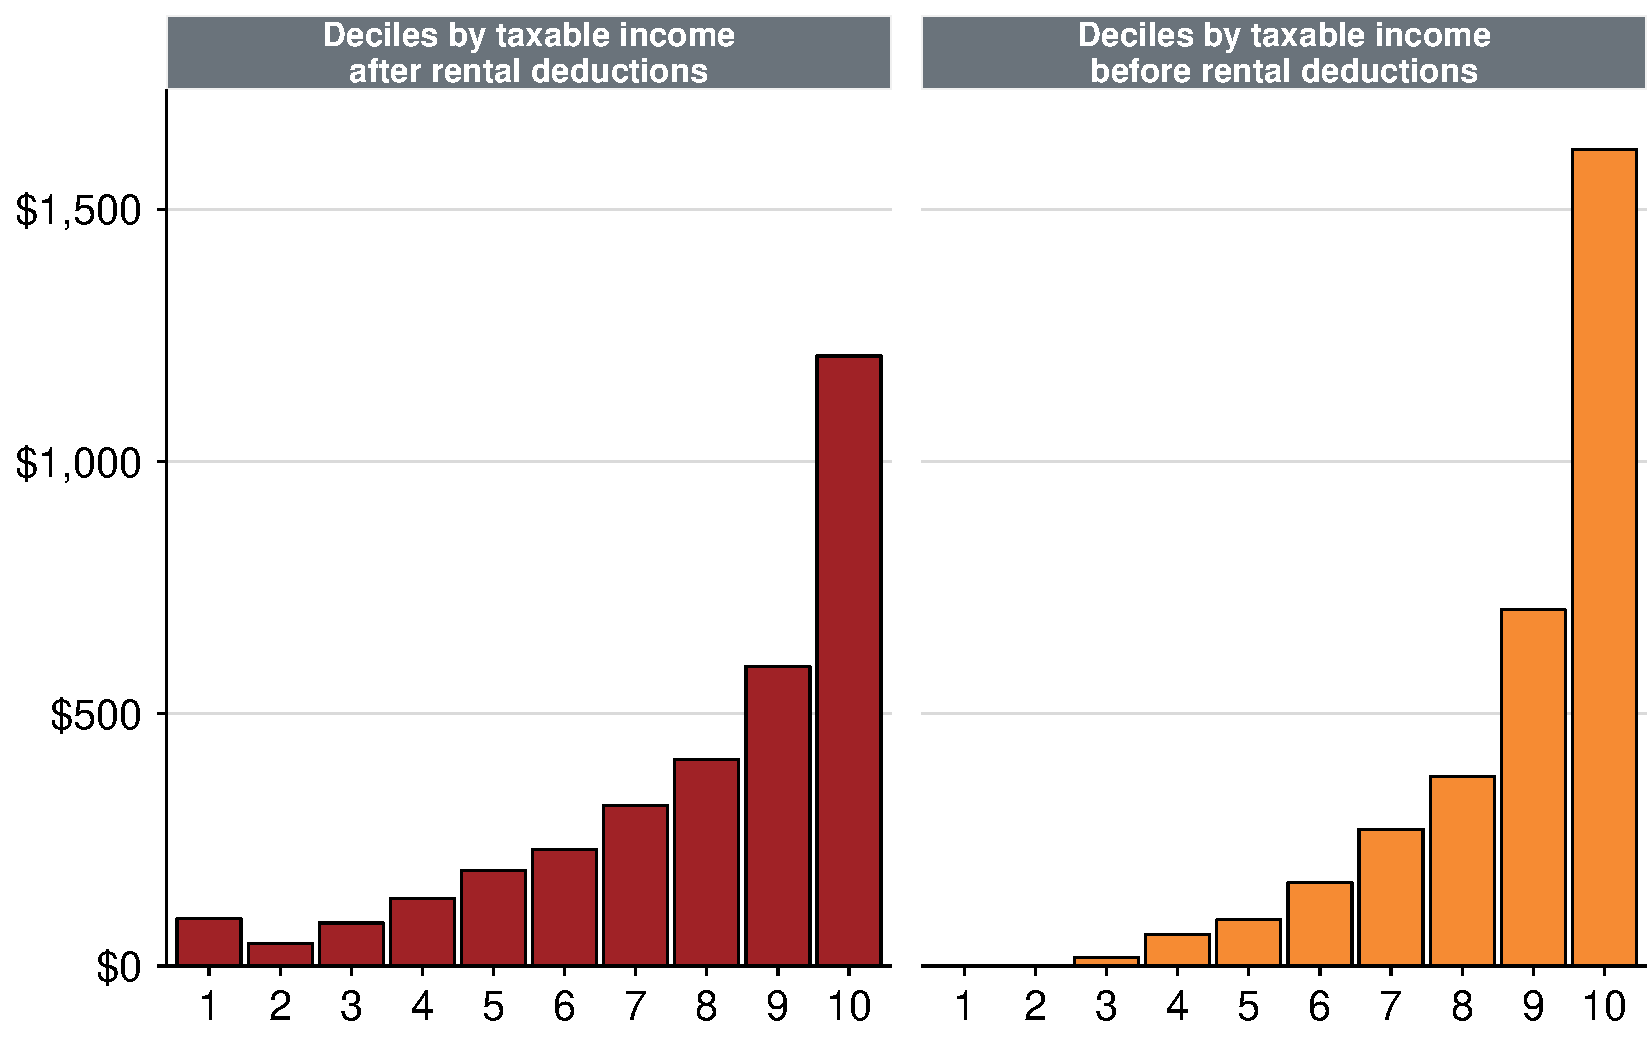
\includegraphics[width=\columnwidth]{figure/Effect_of_Deductions_amount-1}
% \notes{Income tax includes medicare levy,  medicare thresholds, but not other tax benefits (\emph{e.g.}~the seniors and pensioners tax offset (SAPTO))}
% 
% \source{\gao\ \textcite{ATO2013i}}
% \end{figure}

\subsection{Limiting negative gearing should not push up rents}
Concerns persist that limiting negative gearing will reduce the supply of rental properties and push up rents. Some of this seems to reflect folk memory from when the Hawke Government temporarily abolished negative gearing in the 1980s. Rents rose rapidly in Sydney and Perth. But adjusted for inflation, rents were stable in Melbourne and fell in Adelaide and Brisbane (\Vref{fig:Capital_city_rents}). In Sydney and Perth population growth and insufficient new housing, not tax policy, contributed to the rent rise.\footcite[pp.~47-48]{Daley2013}




\begin{figure}
\Caption{Negative gearing does not keep rents low. Only Perth experienced a considerable increase in rents without negative gearing. Adelaide and Brisbane actually experienced declines.}{Average rent prices (real compared with overall CPI), 1983 = 1. Grey band indicates the dates when negative gearing was not permitted}{fig:Capital_city_rents}
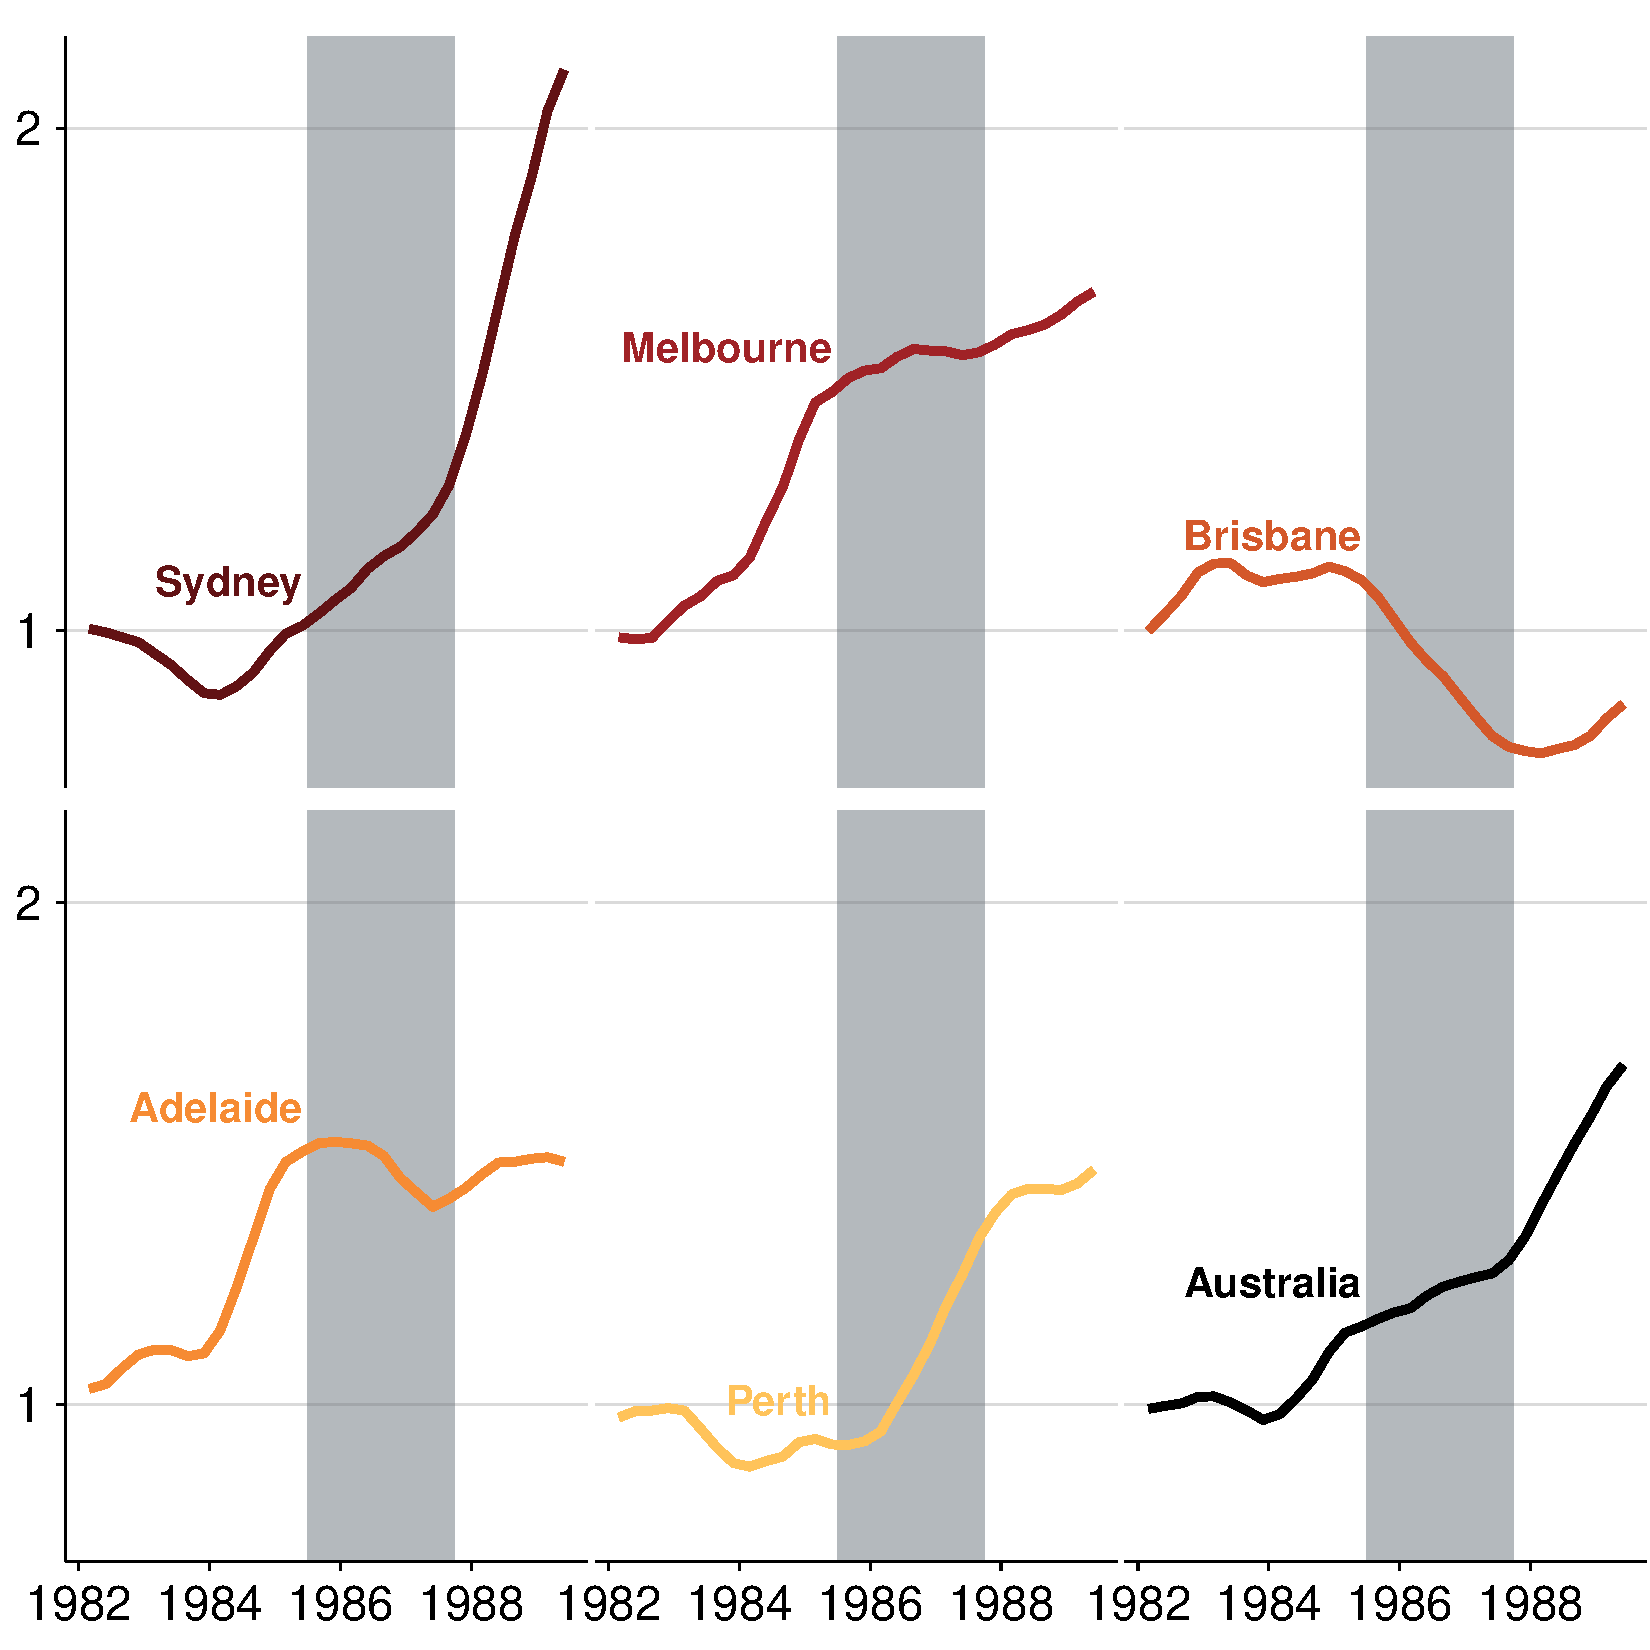
\includegraphics[width=\columnwidth]{figure/Capital_city_rents-1}
\source{ABS various years}
\end{figure}

Economic theory predicts that removing negative gearing should not change rents much. Every time an investor sells a property to a renter, there is one less rental property, and one less renter. There is no change to the balance between supply and demand of rental properties in the short term. 

It is also unlikely that removing negative gearing would affect the supply of new dwellings much over the medium term. Currently 93 per cent of all investment property lending is for existing dwellings.\footcite{ABS2015} Less investor demand would depress overall house prices and therefore returns to new construction.\footnote{The price transmission will be somewhat muted by the fact that the market for new housing, typically at the edge of cities, is somewhat detached from the market for established housing typically closer to the centre \textcite[See]{Kelly2011}.} But the main constraint on new housing is land release and zoning restrictions rather than the profitability of developments.\footcite[pp.84-90]{Kelly2013}

\section{Depreciation allowances also provide substantial tax advantages for investors}
Negative gearing and capital gains tax liabilities also interact to provide overly generous tax advantages to investors through depreciation allowances. 

Allowing capital works deductions for buildings and depreciation of fixtures and fittings is consistent with the principle that the costs of generating taxable income should be deductible.\footcite{Commission2004}  Property investors receive generous depreciation and capital allowances which they can write off in full against their taxable income. Capital works deductions can generally be claimed for construction costs and capital improvements at the rate of 2.5 per cent a year.\footcite{ATO2014b} The decline in value for other fixtures and fittings -- for example, window dressings or whitegoods -- can also be claimed as an expense.\footcite{ATO2014c}

When the asset is sold, the capital gain is based on a cost base calculated from the original purchase price, plus any improvements, less the depreciation claimed.\footcite[p.~21]{ATO2014d} This provides investors with a tax benefit: they write off the allowance at their marginal tax rate, but it is only clawed back at the discounted capital gains rate.\footnote{\textcite{RBA2014}. Most countries have more restricted depreciation allowances for investment housing. Others such as the UK and the Netherlands do not allow any depreciation writes offs. \textcite{Commission2004}}  In effect, investors receive a substantial tax windfall \Vref{box:Tax_advantage_from_capital_works_deductions}.  

\begin{smallbox}{Tax advantage from capital works deductions}{box:Tax_advantage_from_capital_works_deductions}
The property \$750,000 Hayley purchases was built in 1995. Her accountant estimates that the construction cost of the property for capital works deduction purposes is \$250,000, which includes the cost of the house, the pool and the recently constructed patio. 

Hayley claims capital works deductions of 2.5 per cent each year. She holds the property for ten years giving her deductions of \$56,000 over the period. If she remains in the top tax bracket, she receives capital works tax deductions of \$27,400 over the 10 years. 

When she sells the property for \$1 million, her capital gain is the difference between the selling price of the house and the cost base. If she has not made any further improvements to the property, the cost base will be the \$750,000 purchase price minus the \$56,000 in capital works deductions. Hayley's gross capital gain is \$194,000, she pays \$48,000 of this in tax. Because of the capital gains discount, only \$13,700 of the deductions she has claimed on capital works are clawed back through the tax on capital gains.

In effect, the owner nets a windfall for the amount of the capital works deductions claimed, multiplied by half of their marginal rate.
\end{smallbox}
Because of the interaction with the capital gains tax discount, Australia's treatment of depreciation appears to be more favourable than the treatment in other countries.\footcite{RBA2014}

\section{Options for reform}
The favourable tax treatment of investments -- particularly the interaction of the negative gearing arrangements with the capital gains tax discount -- have promoted speculative investment in housing while also costing the budget bottom line. 

Reducing the capital gains tax discount is the most direct way to reduce the incentive for inefficient investment activity. At the same time, negative gearing should be restricted so that losses from investments cannot be deducted against wage and salary income. The tax treatment of depreciation should also be changed to remove the preferential tax advantages generated by the asymmetric treatment of gains and losses. 

Reforms to capital gains tax or eligibility for negative gearing should apply to all types of assets, not just rental properties, so that the tax system does not encourage investors to favour one type of investment over another.  \footcite[p.~133]{Commission2004}

\subsection{Reducing the capital gains tax discount}
Reducing the capital gains tax discount would make the investment tax regime more efficient and fair. 

There are good arguments to abolish the capital gains tax discount altogether. It is not obvious why returns from investment should be taxed less that returns to working. And the differential tax rates create incentives for people to convert labour into capital income. 

But the arguments advanced for maintaining concessional treatment of gains sound a word of caution. While there is no compelling evidence that changes in tax rates materially change savings and investment behaviour, most studies examining these issues look at changes in behaviour in response to relatively modest changes in tax rates. Eliminating the capital gains tax discount would at least double the effective tax rate paid on capital returns. No OECD country taxes capital gains at full marginal tax rates in all circumstances. 

A more cautious approach would be to reduce the discount. Reducing the discount to 30 per cent, could raise around \$4 billion. Because this estimate does not include the effect on asset prices and investor behaviour, actual revenue raised is likely to be somewhat lower. On the other hand, these revenues should rise over time as capital losses built up from the GFC pass through the system.\footnote{CGT revenues are yet to recover following the GFC. Receipts were 0.46 per cent of GDP in 2012-13, down from a peak of 1.56 per cent of GDP in 2007-08. Even as asset prices have improved, capital losses carried forward have limited taxable gains. \textcite{Stewart2015}; \textcite{PBO2014}. }

This proposal would also be strongly progressive. Taxing capital gains in the same way as income would have very little effect on the tax burden for those in the bottom 20 per cent of the income distribution that earn little in the way of gains, as shown in \Vref{fig:Nearly_eighty_per_cent_of_capital_gains_are_earned_by_those_}. 

Reducing the discount will not entirely eliminate the distortions in investment decisions from the asymmetric treatment of gains and losses, but it will go some way towards it particularly if done in conjunction with limiting the deductibility of losses (see below). 

A partial removal of the discount, particularly if introduced slowly over time (\Vref{sec:transitional_arrangements}), will allow monitoring of the effects on investment markets. 

\subsection{Limiting negative gearing}
There is also a strong case for limiting the tax deductibility of losses. Quarantining losses so they cannot be written off against wage and salary income would limit the current distortions. 

While the deductibility of investment expenses including income expenses, has a strong grounding, there is no reason that these expenses should be deducted against wage and salary income.

This proposal would raise additional tax revenue in the short term, although the estimates are sensitive to changes in the housing market and the holding periods for assets. Applying the average marginal tax rate to the average annual rental losses of \$10.4 billion would yield \$4.2 billion in additional tax revenue in the short-term. 

Over the medium term, rental losses will start to be written off against income from capital gains. Assuming no change in investor behaviour, the additional tax revenue net of lower capital gains tax revenue would revert to around its average level of \$1.5 billion a year. 

But behavioural change is likely. Investments that make income losses are less attractive when the tax benefits can only be realised on sale. Much of the appeal of negative gearing lies in the scope to reduce annual taxes on wage income (\Vref{sec:negative_gearing_provides}). Removing the tax incentive for leveraged investment should result in investors shifting toward income producing assets and therefore an overall increase in income tax collections.  

\subsection{Matched discount and claimable losses}
An alternative proposal put forward in the Henry review was to discount rental losses by the same amount as the capital gains tax discount.\footcite[pp.~70,72]{Treasury2010}  In other words, only 50 per cent of expenses (including interest) associated with investments would be allowed as deduction against wage and salary income.  This proposal could also raise an additional \$2 billion each year for the budget. 

By restoring the symmetry in the treatment of gains and losses, investors would have less incentive to `chase' capital gains rather than recurrent income.\footcite[p.~418]{Treasury2010}

\subsection{Improve tax treatment of depreciation}
If capital gains tax discounts remain in place, then the taxation of depreciation allowances should also be reformed. When an asset is sold and the sale price is more than the purchase price, depreciation should not be deducted from the cost base for the purposes of calculating the capital gain. Instead, the tax deduction already received for depreciation should be refunded in full.\footnote{This is a variant of a proposal recommended by Rider and Stewart in their submission to the Productivity Commission Review of First Home Ownership. \textcite{Rider2004}}

This would remove the current tax advantage for depreciation because discounted capital gains tax arrangements only recoup half of the depreciation deductions claimed (section 1.4).  Each year around \$2 billion dollars is claimed in capital works allowances. If the depreciation previously claimed on these works were fully refunded, rather than recouped at the 50 per cent capital gain tax rate, this would raise up to an additional \$1 billion each year.\footnote{This estimate only includes building and capital works deductions and not depreciation for fixtures and fittings which are not reported separately by the ATO.  It does not include estimates of any behavioural change. It also assumes that investors are in the same tax bracket when the asset is sold as when the depreciation deductions are claimed. Because of the incentives to realise assets when tax rates are low this is an upper end estimate}

Investors would continue to receive the generous tax deferral advantages of the current depreciation regime.\footnote{Arguably current depreciation allowances are higher than the real economic depreciation of fixtures and fittings. Investors have an incentive to claim the maximum allowances. See \textcite[pp.~130-131]{Commission2004}.}

\section{Transitional arrangements}\label{sec:transitional_arrangements}
Whether governments choose to reform capital gains tax or negative gearing arrangements, changes should be phased-in to minimise sudden shifts in asset markets that are prone to over-shooting. Phase-in also provides investors with time to reorganise their affairs to adjust to the new regime.

Immediate reform to the current capital gains discount or negative gearing regimes would encourage investors to sell before the new legislation came into force. This could be moderated by phasing in the changes over a number of years. For example, under a ten year phase-in, the capital gains discount could be reduced to 45 per cent in the first year, and then reduced by five percentage points each year until all capital gains are taxed at the full marginal rate. Similarly, changes to Negative gearing could be phased in. For example, taxpayers might be allowed to claim only 90 per cent of their losses against wage and salary income in the first year (the remainder capitalised against any future capital gain), and the ten percentage points less each year until no losses are claimed against wage and salary income.

A less preferable alternative would be to grandfather existing arrangements. Those who purchased assets before capital gains tax reform was implemented could still claim the capital gains tax discount, even if they sell the assets several years afterwards. Similarly, those who purchased assets before negative gearing reform, could continue to claim all of their losses against their wage and salary income until the asset was sold.

Grandfathering causes a number of problems: it adds to complexity, reduces liquidity, and treats investors -- particularly younger investors -- unfairly.

Applying different tax treatments to investments depending on when they were acquired adds to the complexity of the tax system. Because investors can hold assets for decades, these dual tax arrangements are long-lived.  For example, the decision to grandfather the capital gains tax free status for assets purchased before 1986 still contributes to the complexity of our capital gains tax regime, 29 years later.\footcite[p.~75]{Treasury2010} 

Grandfathering arrangements reduce liquidity because investors have substantial incentives to retain whichever assets they purchased before the reform was implemented. They will be reluctant to buy and sell because the after tax returns on the assets bought earlier will be higher. Such a drag on liquidity is economically inefficient because it encourages investors to hold assets even when others could extract a higher return from them. This is a particular concern with negative gearing where a landlord may continue to hold a property because it generates ongoing deductible losses, even though an alternative owner might profitably develop the property. Grandfathering also exacerbates intergenerational inequality.\footcite{Daley2014}  Those who own assets before the reforms -- more likely those who are older -- earn higher after tax returns than those who start to build wealth later on.\footcite[p.~14]{Daley2014} 

Grandfathering arrangements are often driven by the principle of retrospectivity. However, this principle is often misunderstood. Concerns arise if a person acts as they would not otherwise because of a government policy, and then that policy changes to their detriment. Legitimate expectations, for which government is responsible, are defeated. But the concerns are much weaker if the person would have acted in the same way even if the new policy had been in place.

This is particularly relevant if the capital gains tax regime is changed for all asset classes. The after tax return for all asset classes (other than bank deposits) would be affected simultaneously. It is not obvious that investors would have saved less if there had been no capital gains tax discount.\footnote{Tax incentives for savings have greater effect on the choice of investment vehicle rather than the overall savings rate (see section 5.2 for discussion).} However, investors might have invested differently. In particular, they might well have invested less in property without the attraction of the negative gearing arrangements. 

Nor is the principle of retrospectivity absolute. Governments are entitled to change tax rates. If a person buys BHP Billiton shares, they cannot expect that the marginal tax rate then in force will still apply when they sell. No investor is entitled to a particular after-tax return in perpetuity.

Grandfathering (rather than a phase-in) may help existing owners less than they think. Abolishing the capital gains discount or restricting claims for losses on investments would reduce the after-tax returns for new purchasers. This would reduce the price they are prepared to pay existing owners.\footnote{This assumes that demand is dominated by potential new owners who would be affected by the new tax arrangements. An alternative approach would identify the "marginal investor", and expect a change in price only if they were affected by the new tax regime. In reality, demand is inevitably a combination of potential investors, subject to a variety of tax regimes, and the effect on price will depend on the extent of the tax change, and the proportion of potential investors affected.} A phase-in -- which treated old and new owners alike -- would have less immediate price impacts.

If grandfathering is nevertheless adopted, complexity in the long-term might be reduced by a sunset clause. This would provide that the new tax arrangements would apply to assets bought before the reforms if they were sold more than (say) fifteen years after the reform. This would provide existing owners ample time to reorganise, few investment assets are held for this long, and it would reduce complexity in the long-term.

The most powerful argument for grandfathering is political economy: those who benefit from the current arrangements are likely to be the most vociferous opponents of reform. It may be better to grandfather existing arrangements -- thereby muting opposition -- than to abandon worthwhile reform altogether.  
Nevertheless, given the competing considerations, phase-in would be a better transition. There would be less complexity, less immediate impact on prices, and younger investors would be treated more fairly. Concerns about investor expectations are not particularly strong as the phase-in proposed would provide them with ample time to reorder their affairs.







\begin{figure}
\Caption{}{Number of taxpayers by taxable income decile who negatively gear}{fig:NegGearing_share_by_deciles}
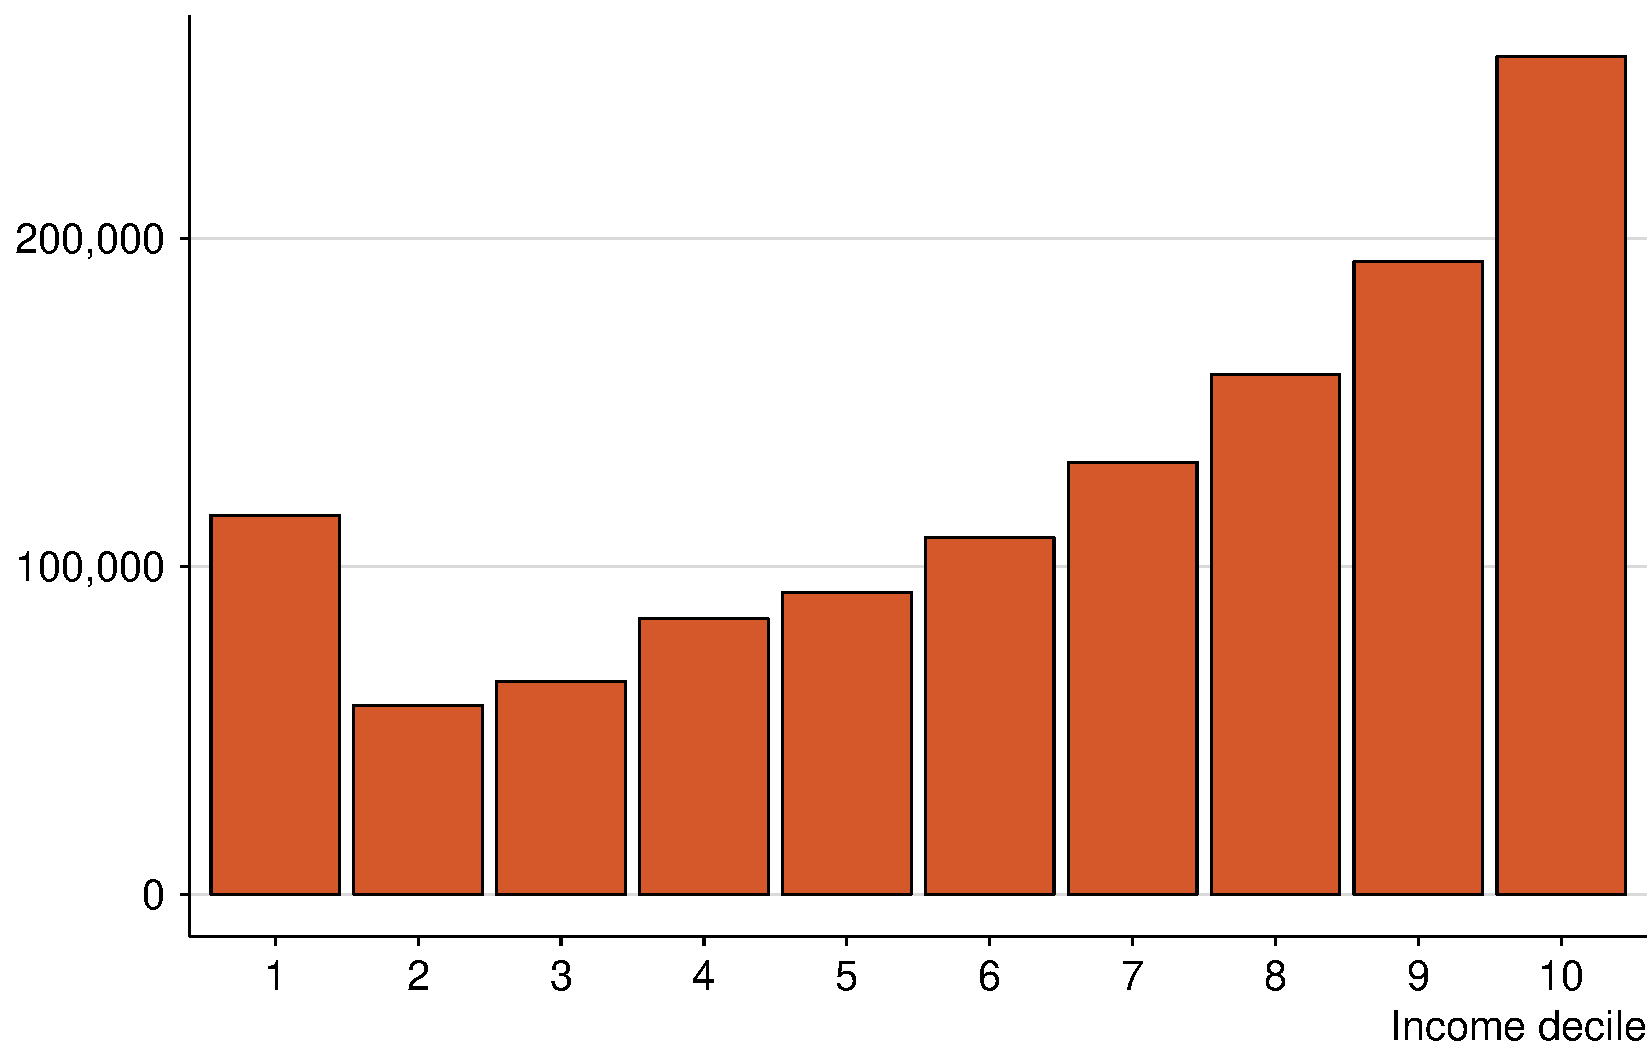
\includegraphics[width=\columnwidth]{figure/NegGearing_share_by_deciles-1}
\notes{}

\source{}
\end{figure}



\begin{figure}
\Caption{}{Total net rental losses by taxable income decile}{fig:NegGearing_amount_by_deciles}
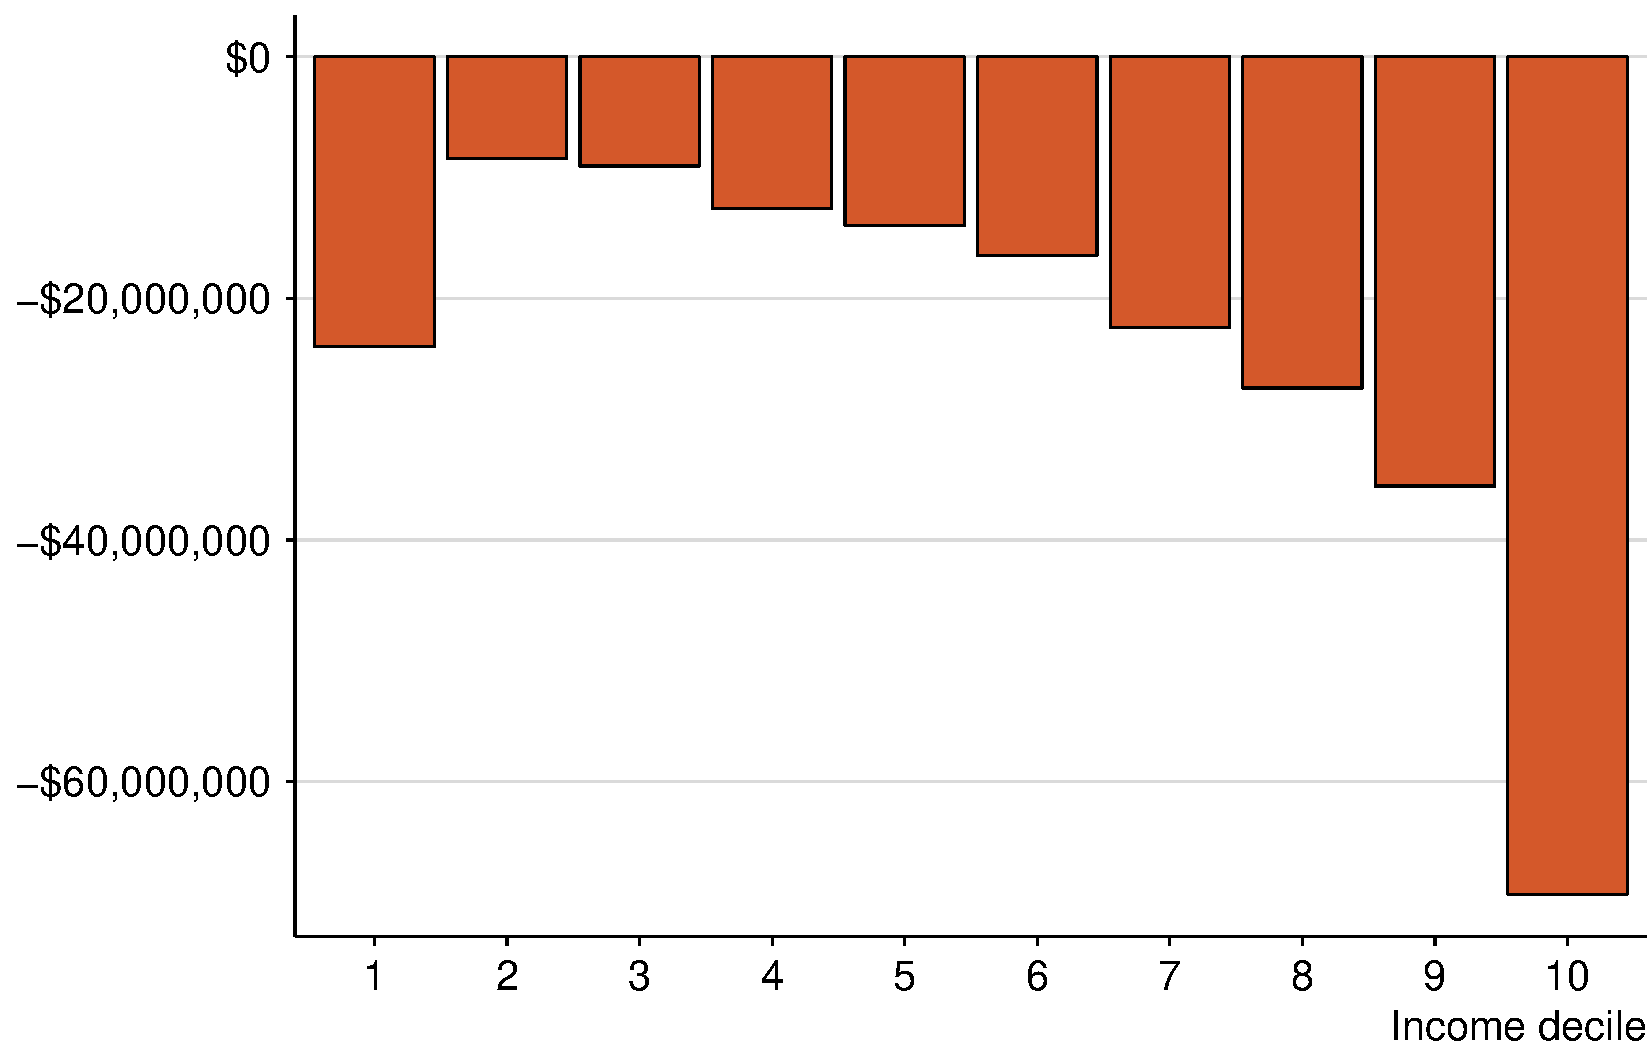
\includegraphics[width=\columnwidth]{figure/NegGearing_amount_by_deciles-1}
\notes{}

\source{}
\end{figure}



\begin{figure}
\Caption{}{Average rental losses (for those with negative net rental amounts)}{fig:NegGearing_avg_amount_by_deciles}
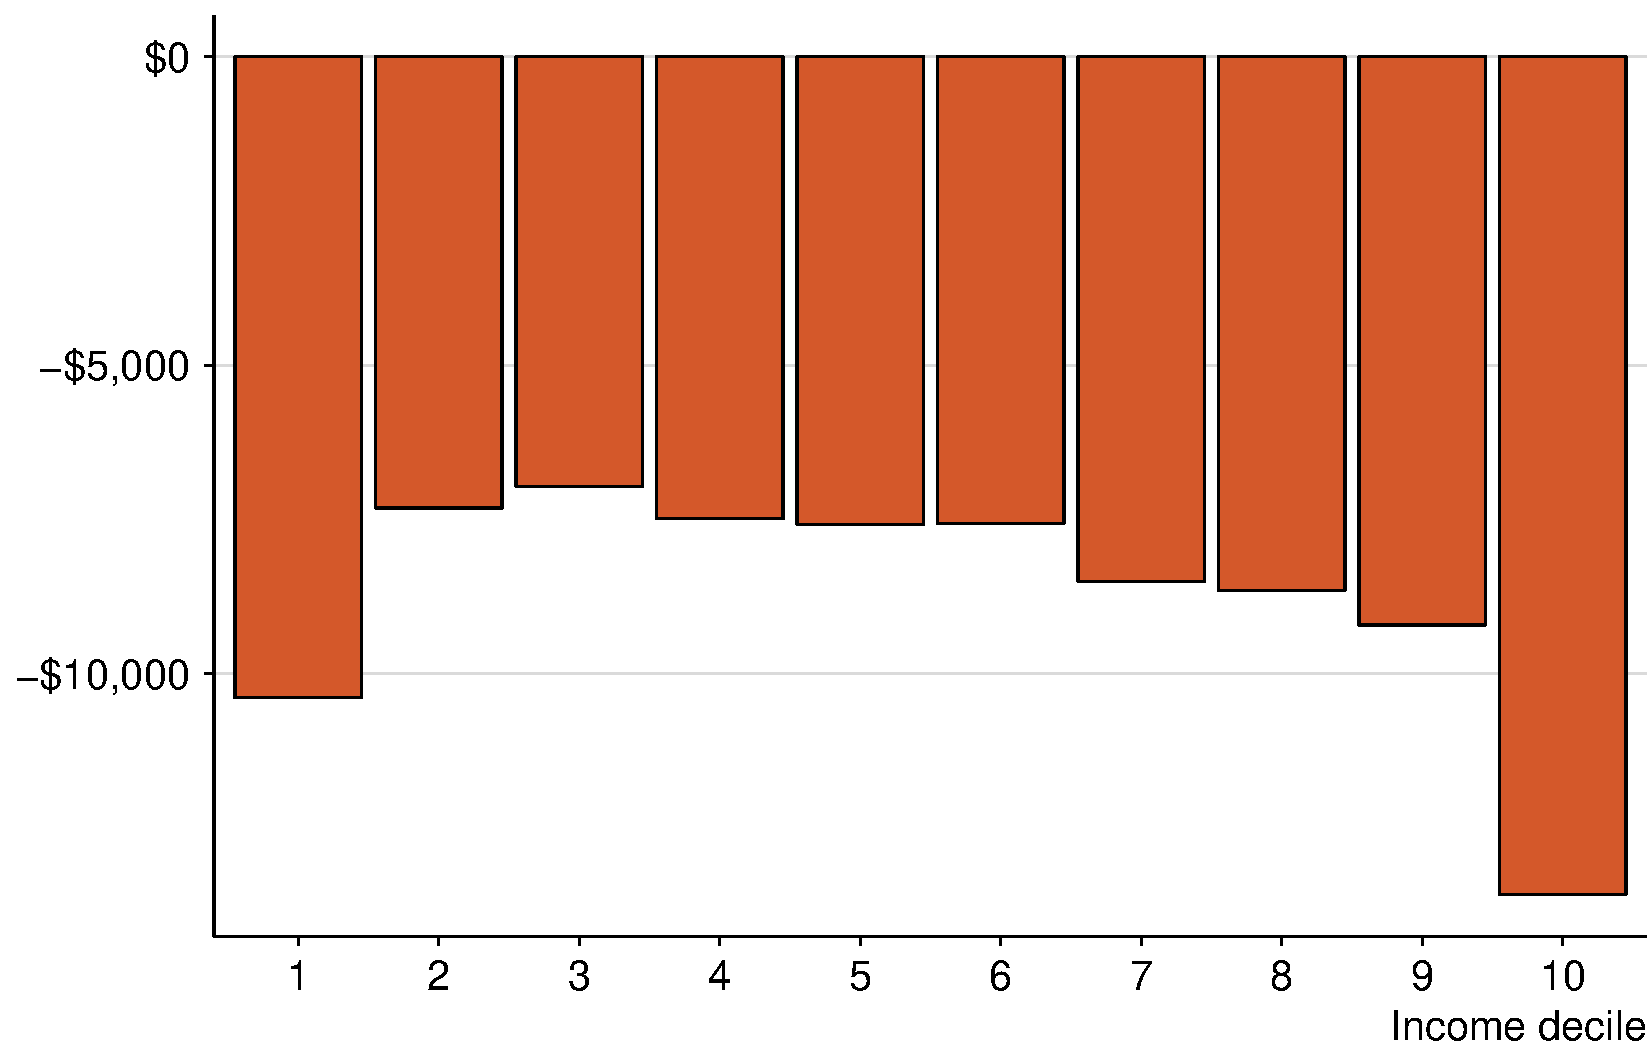
\includegraphics[width=\columnwidth]{figure/NegGearing_avg_amount_by_deciles-1}
\notes{}

\source{}
\end{figure}



\begin{figure}
\Caption{A higher proportion of taxpayers from the top income tax brackets change brackets as a consequence of negative gearing}{Number and proportion of taxpayers in each tax bracket (income determined before rental deductions) who change brackets as a result of negative gearing}{fig:Tax_brackets}
\includegraphics[width=\columnwidth]{figure2/Tax_brackets-1}
\notes{}

\source{\gao \textcite{ATO2013i}}
\end{figure}

\begin{figure}
\Caption{Negative gearing results in over 200,000 taxpayers moving down at least one tax bracket}{Number of taxpayers moving down tax brackets as a result of rental deductions}{fig:BracketFall}
 \begin{tikzpicture}[node distance = 3cm, auto]
 \tikzstyle{every node}=[font=\small]
  \node [block, fill=Color1] (Under) {0-18,200};
  \node [block, fill=Color2, above right of = Under] (Low) {18,201-37,000};
  \node [block, fill=Color3, above right of = Low] (Middle) {37,001-80,000};
  \node [block, fill=Color4, above right of = Middle] (Upper) {80,001-180,000};
  \node [block, fill=Color5, above right of = Upper] (High) {180,000+};
  %
  \path [line] (Low) --node{41,800} (Under);
  %
  \path [line] (Middle) to[out = 180, in = 90, anchor=west, fill=white]node{8450} (Under);
  \path [line] (Middle) --node{66,650} (Low);
  %
  \path [line] (Upper) --node{84,300} (Middle);
  \path [line] (Upper) to[out = 180, in = 90, anchor=south east]node{1400} (Under);
  \path [line] (Upper) to[out = -90, in = 0] node{1400} (Low);
  %
  \path [line] (High) --node[anchor=south east]{17,650} (Upper);
  \path [line] (High) to[out = 180, in = 90, anchor=south east]node{200} (Middle);
  \path [line] (High) to[out = -90, in = 0]node{100} (Under);
 \end{tikzpicture}
\end{figure}


% latex table generated in R 3.2.0 by xtable 1.7-4 package
% Mon Jun 22 15:49:47 2015
\begin{table}[ht]
\centering
\begin{tabular}{lr}
  \hline
Age & Number negatively gearing \\ 
  \hline
under 20 & 200 \\ 
  20 to 24 & 17,600 \\ 
  25 to 29 & 94,350 \\ 
  30 to 34 & 150,500 \\ 
  35 to 39 & 163,950 \\ 
  40 to 44 & 182,300 \\ 
  45 to 49 & 177,250 \\ 
  50 to 54 & 185,050 \\ 
  55 to 59 & 151,200 \\ 
  60 to 64 & 88,450 \\ 
  65 to 69 & 34,550 \\ 
  70 and over & 15,900 \\ 
   \hline
\end{tabular}
\end{table}



\begin{figure}
\Caption{The incidence of negative gearing is roughly constant for middle-aged Australians. Between 12.9\%\ and 14.8\%\ of each age group from 35 to 59 experience a net rental loss}{Percentage of taxpayers with a net rental loss, by age group}{fig:Percentage_of_taxpayers_with_a_net_rental_loss_by_age_group}
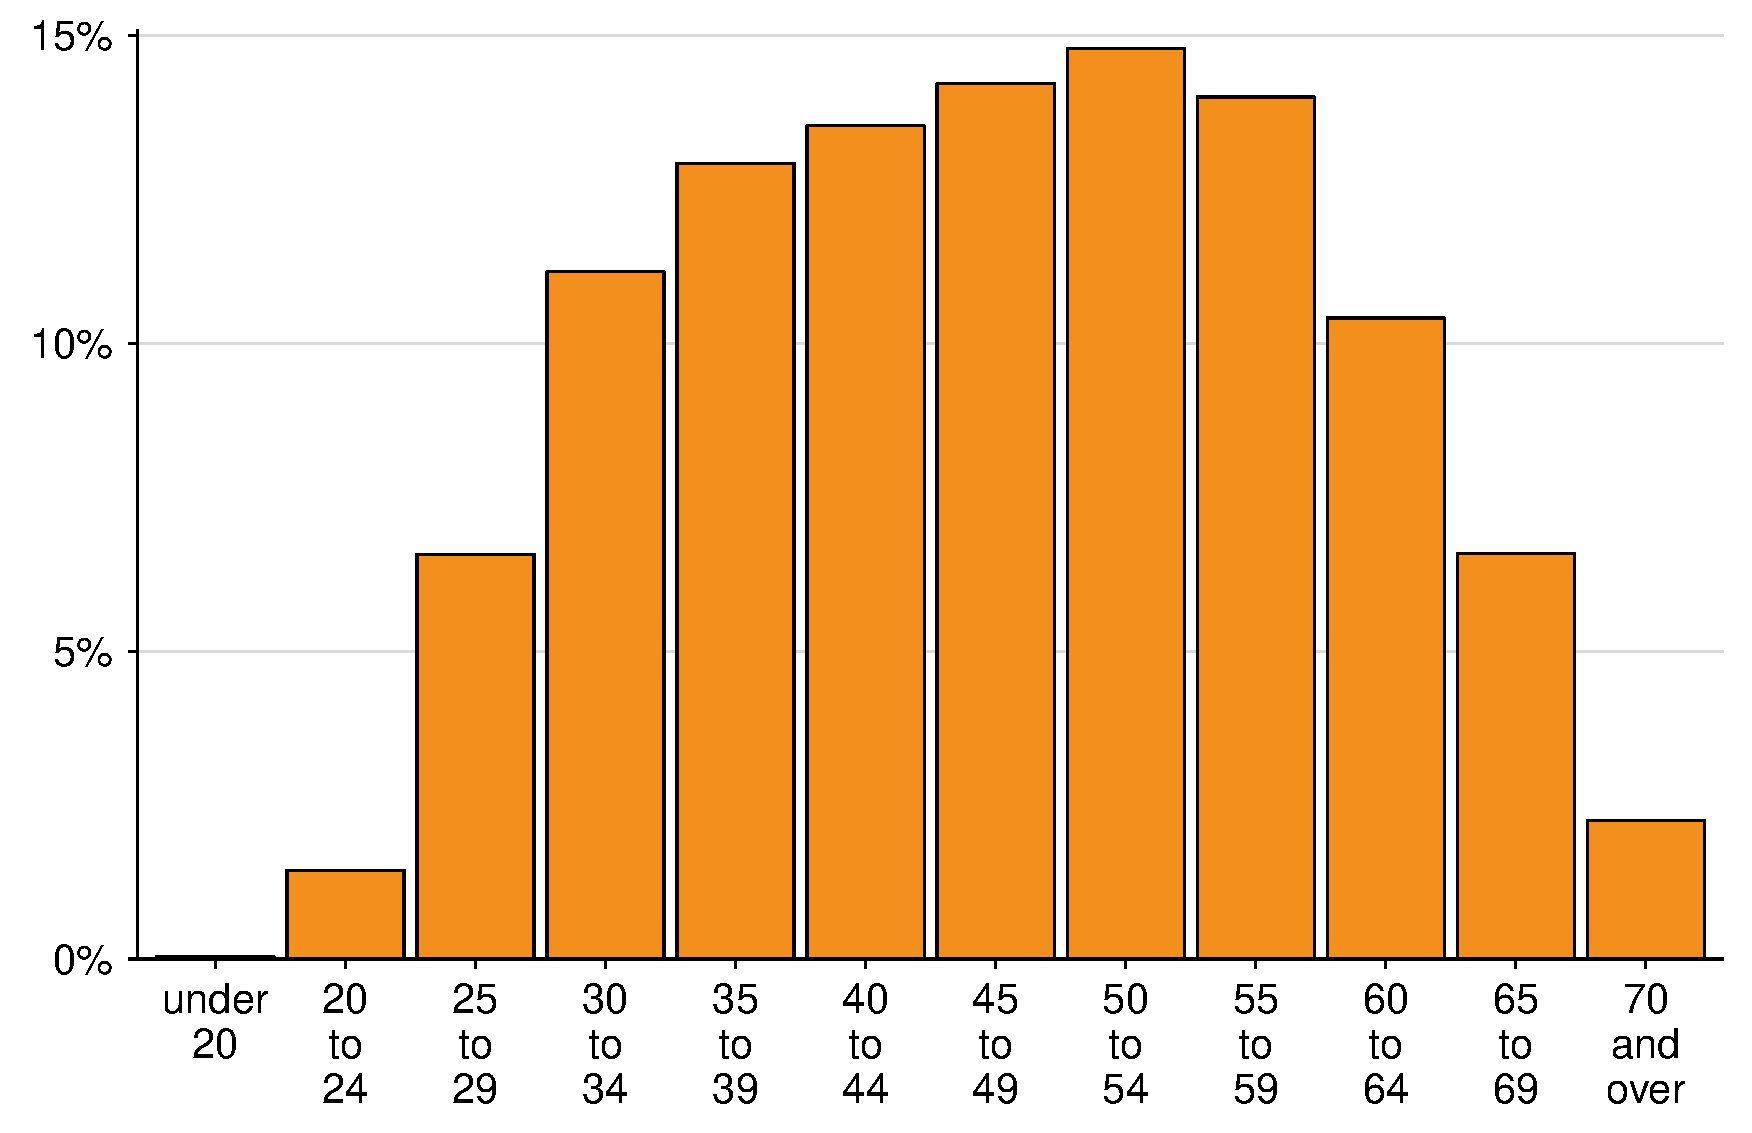
\includegraphics[width=\columnwidth]{figure/Percentage_of_taxpayers_with_a_net_rental_loss_by_age_group-1}
\notes{}

\source{\gao \textcite{ATO2013i}}
\end{figure}



\begin{figure}
\Caption{}{Number of taxpayers by type}{fig:Age_negative_gearing_not_negative_gearing}
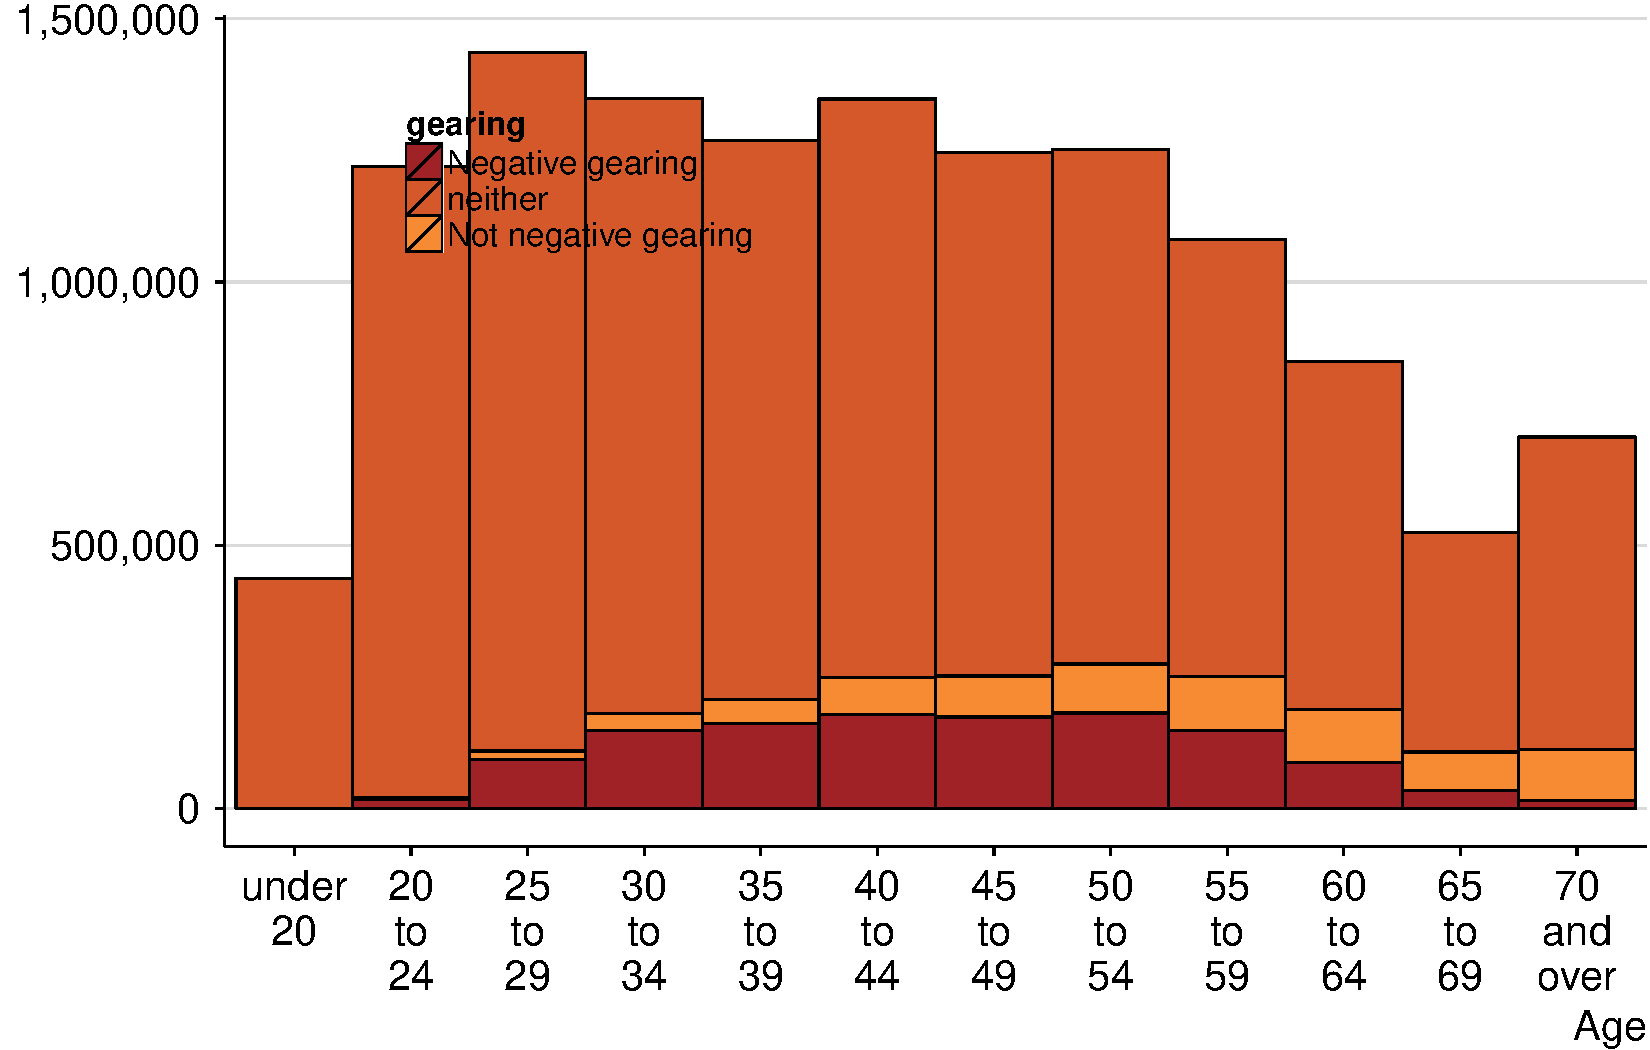
\includegraphics[width=\columnwidth]{figure/Age_negative_gearing_not_negative_gearing-1}
% \source{~\verb!Age_negative_gearing_not_negative_gearing!}
\end{figure}



\begin{figure}
\Caption{Most people with investment properties use negative gearing}{Percentage of each age group with positive rental income with net rental losses}{fig:Negatively_geared_investors_as_a_share_of_all_property_investors_by_age}
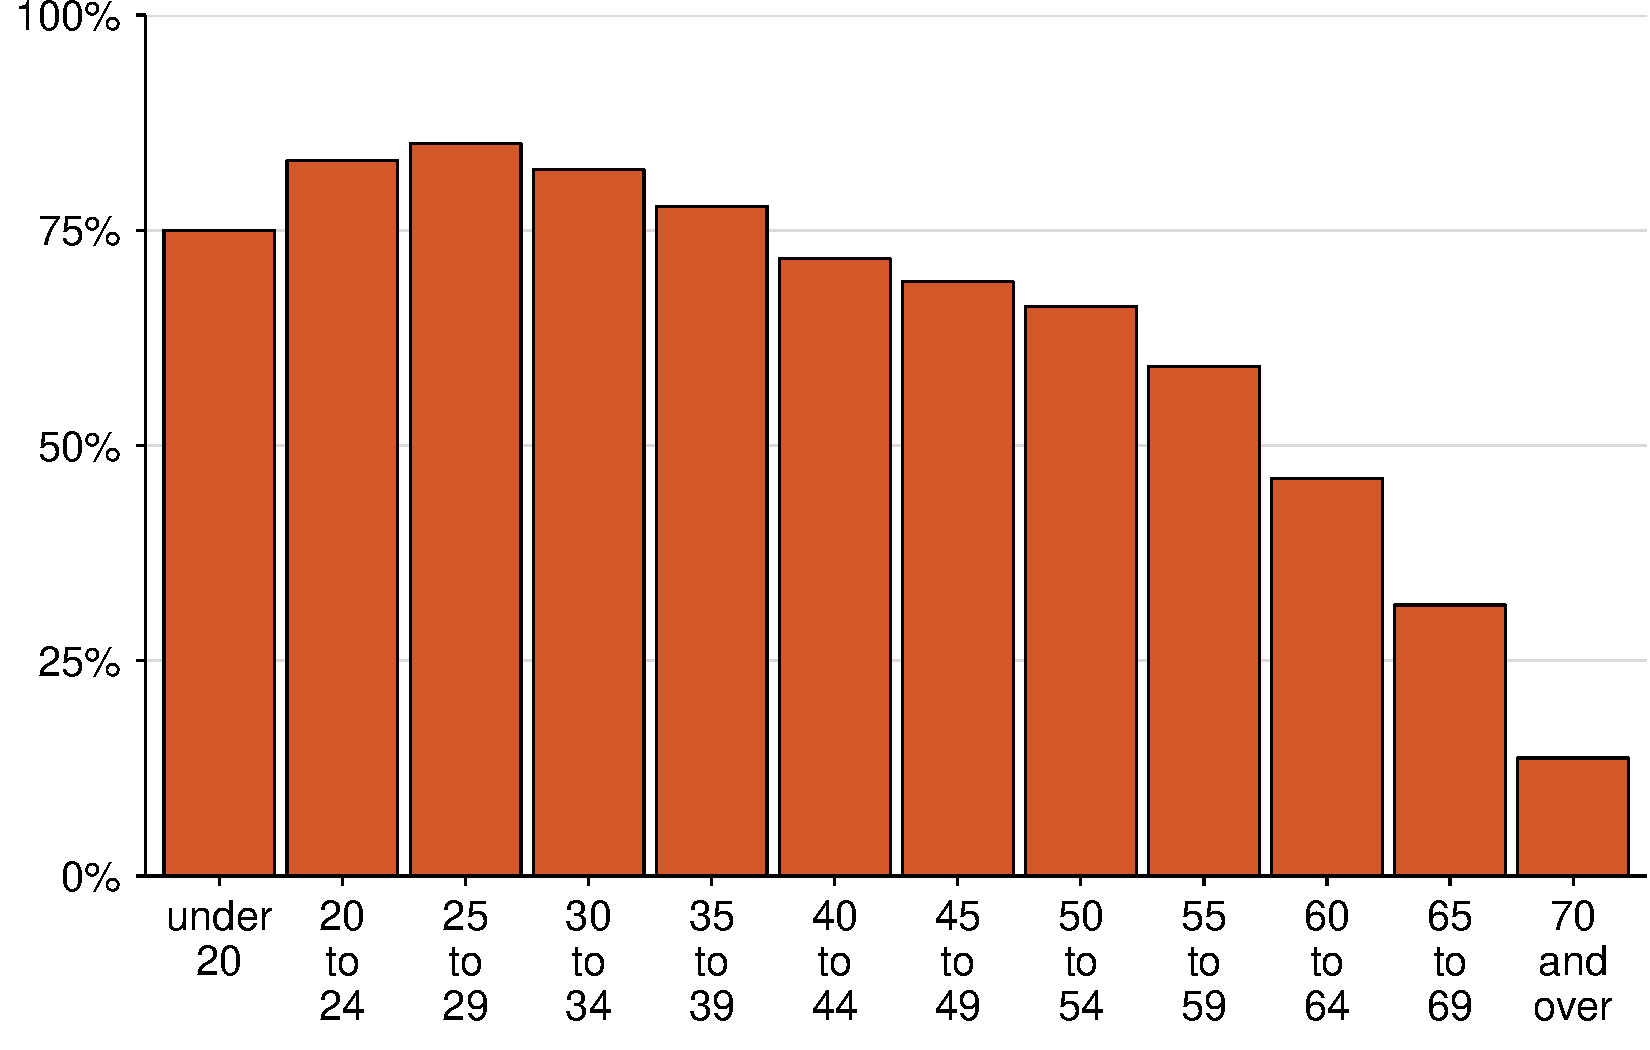
\includegraphics[width=\columnwidth]{figure/Negatively_geared_investors_as_a_share_of_all_property_investors_by_age-1}
\notes{Under 20 age group based on merely four entries in the sample file; only a tiny number of under 20s have investment properties.}

\source{\gao\textcite{ATO2013i}}
\end{figure}

\section{Capital gains distribution}
% Capital gains by income decile.

\begin{figure}
\Caption{Over two-thirds of capital gains are earned by the top 10\%\ of taxpayers}{Average net capital gains by income decile (2012-13)}{fig:Capital_gains_by_income_decile}
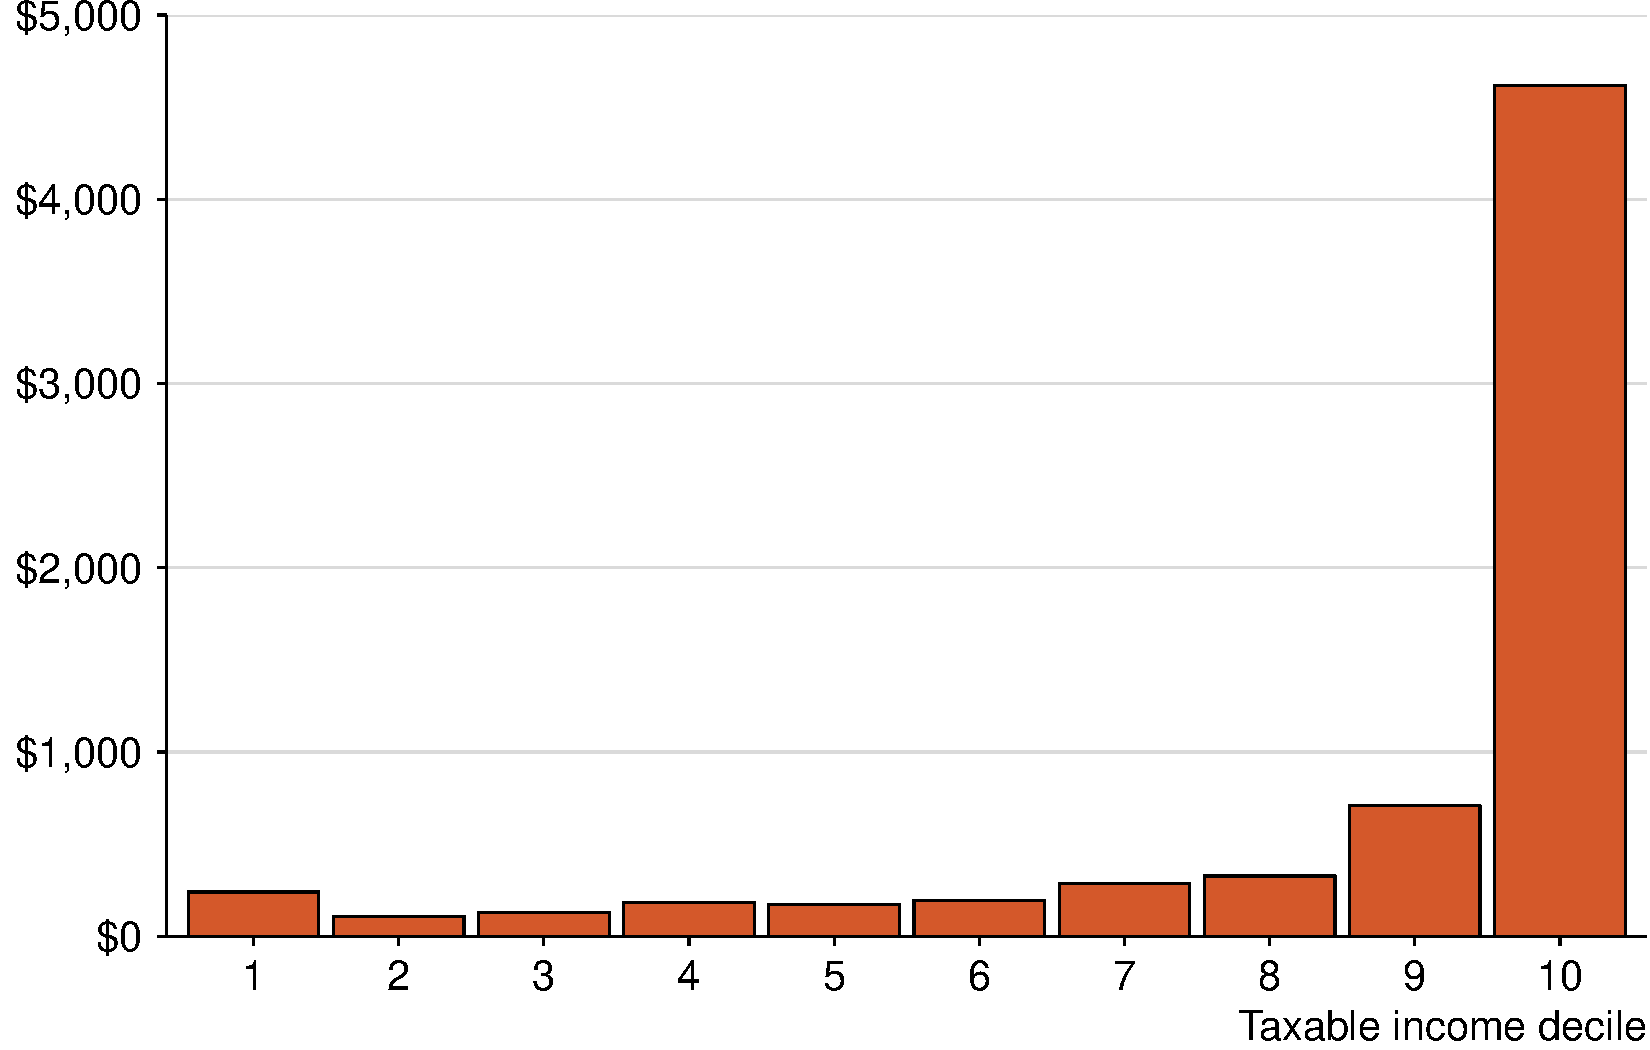
\includegraphics[width=\columnwidth]{figure/Capital_gains_by_taxable_income_decile-1}
\notes{Income based on total income reported}

\source{\gao\ \textcite{ATO2013i}}
\end{figure}


\begin{figure}
\Caption{Capital gains are lumpy}{Average net capital gains by income decile}{fig:Capital_gains_by_taxable_income_without_CG_decile}
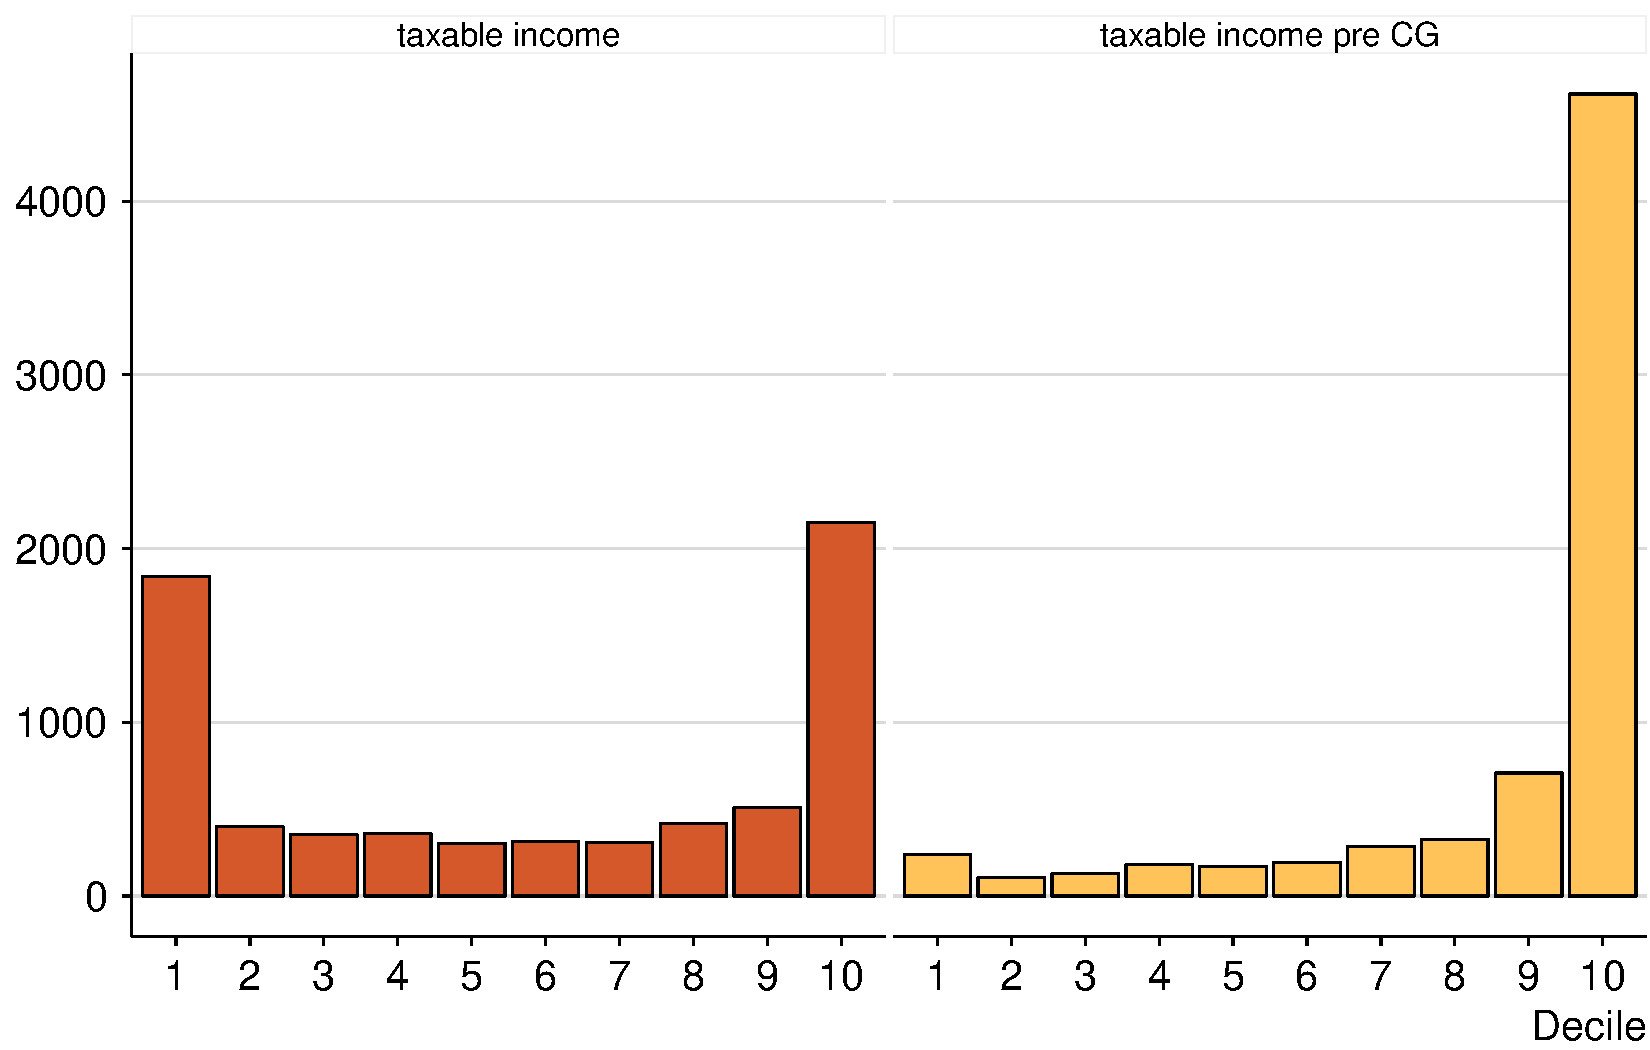
\includegraphics[width=\columnwidth]{figure/Capital_gains_by_taxable_income_without_CG_decile-1}
\source{\gao\ \textcite{ATO2013i}}
\end{figure}




\begin{figure}
\Caption{Net capital gains by age}{\$ billions}{fig:Net_capital_gains_by_age}
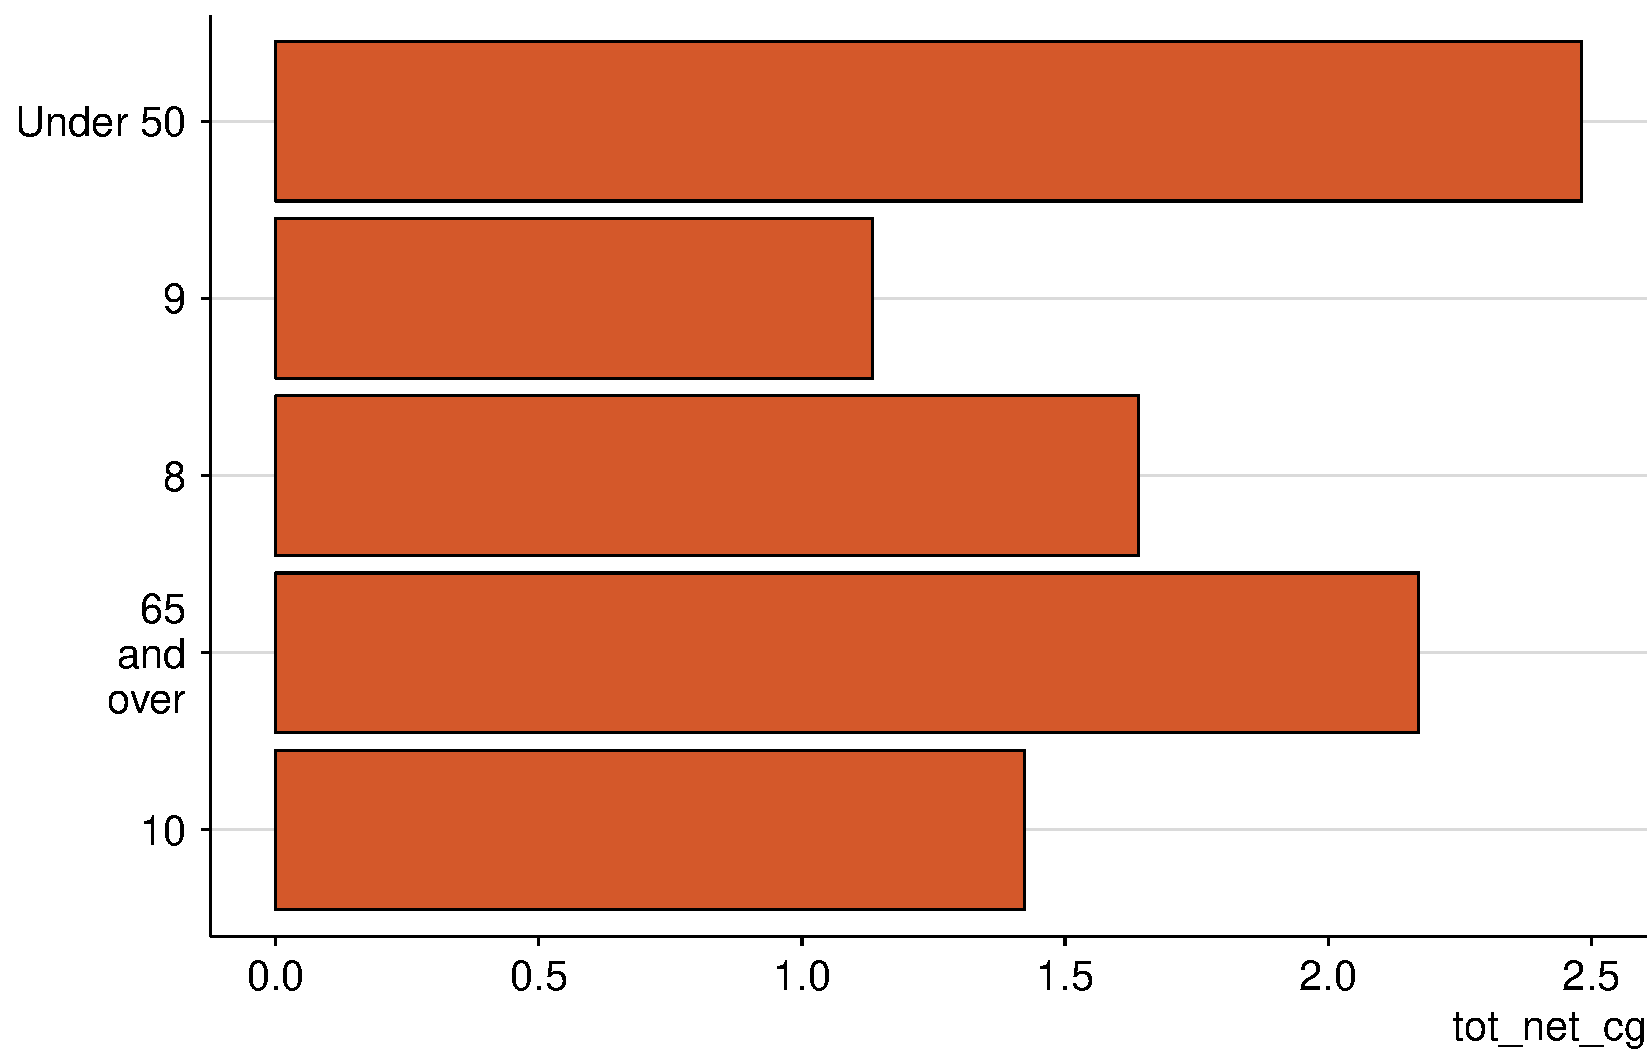
\includegraphics[width=\columnwidth]{figure/Net_capital_gains_by_age-1}
\notes{Net capital gains here are valued after the 50\%\ discount is applied.}

\source{\gao\ \textcite{ATO2013i}}
\end{figure}






\begin{figure}
\Caption{Asset lock-in}{Average net capital gain, by income (excl. CG) decile, by age}{fig:Net_capital_gains_by_age_by_decile}
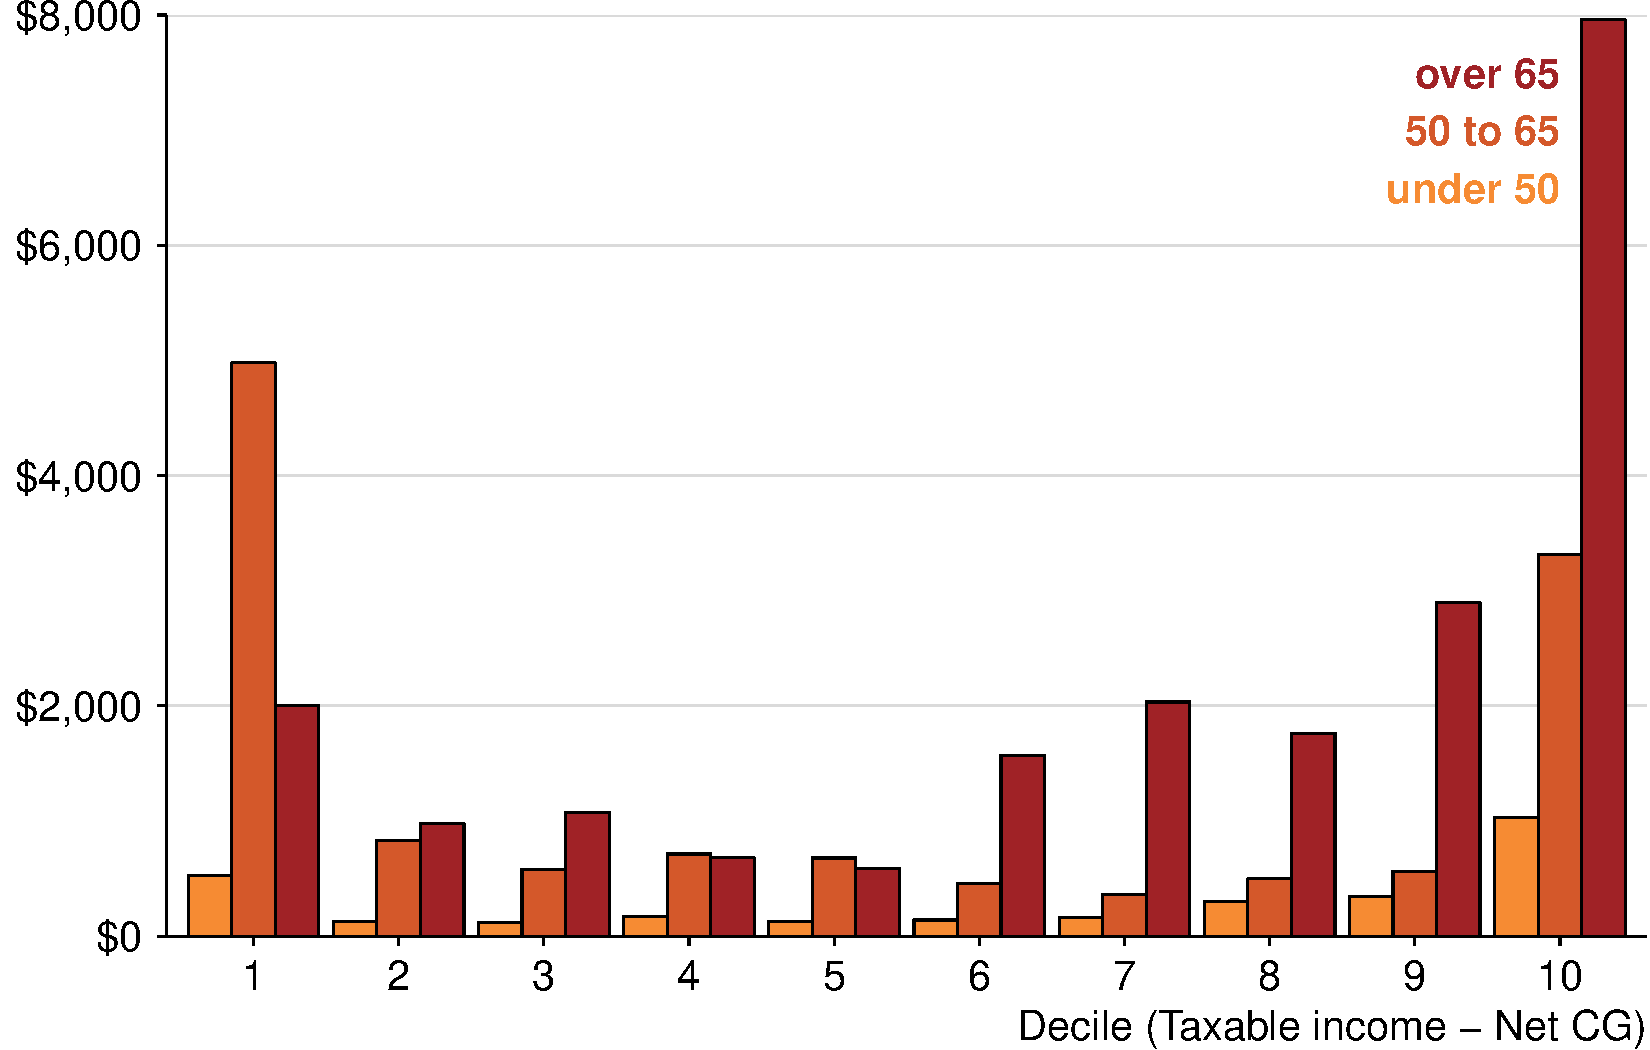
\includegraphics[width=\columnwidth]{figure/Net_capital_gains_by_age_by_decile-1}
\end{figure}


\begin{figure}
\Caption{}{Proportion of each decile and age with positive salary or wages}{fig:Prop_working_by_age_by_decile}
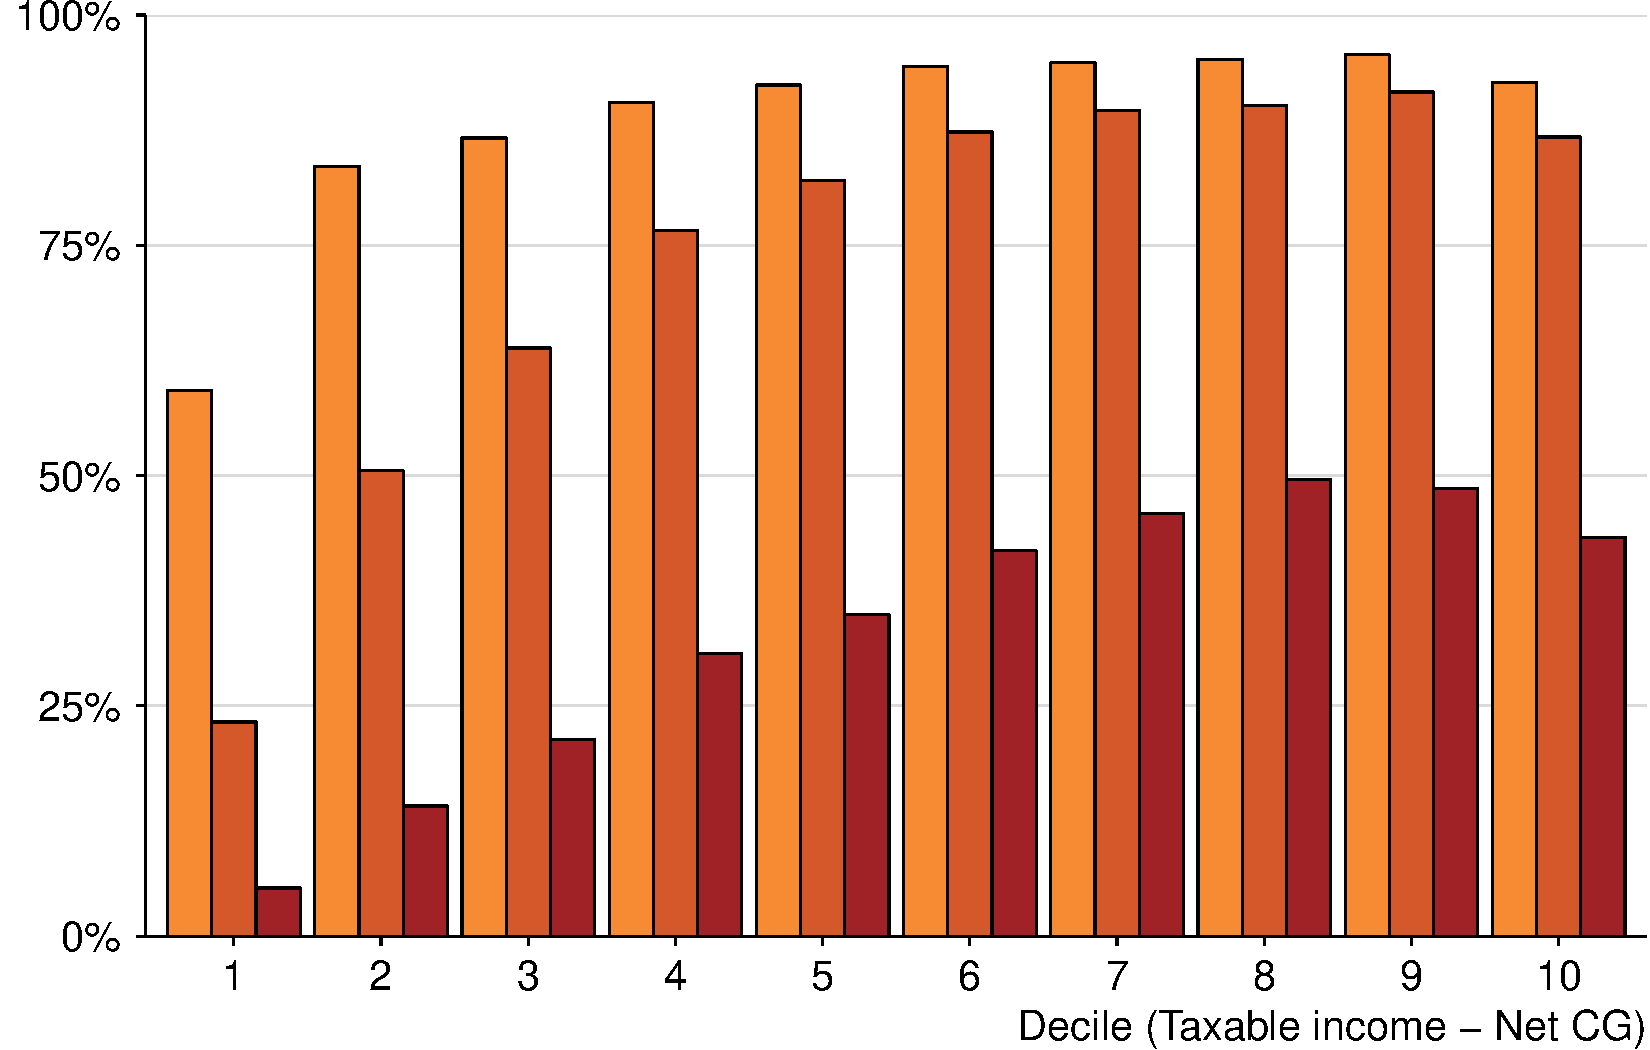
\includegraphics[width=\columnwidth]{figure/Prop_working_by_age_by_decile-1}
\source{\gao\ \textcite{ATO2013i}}
\end{figure}


\begin{figure}
\Caption{Average net capital gains by income decile, taxpayers over 60}{}{fig:Net_capital_gains_decile_over60}
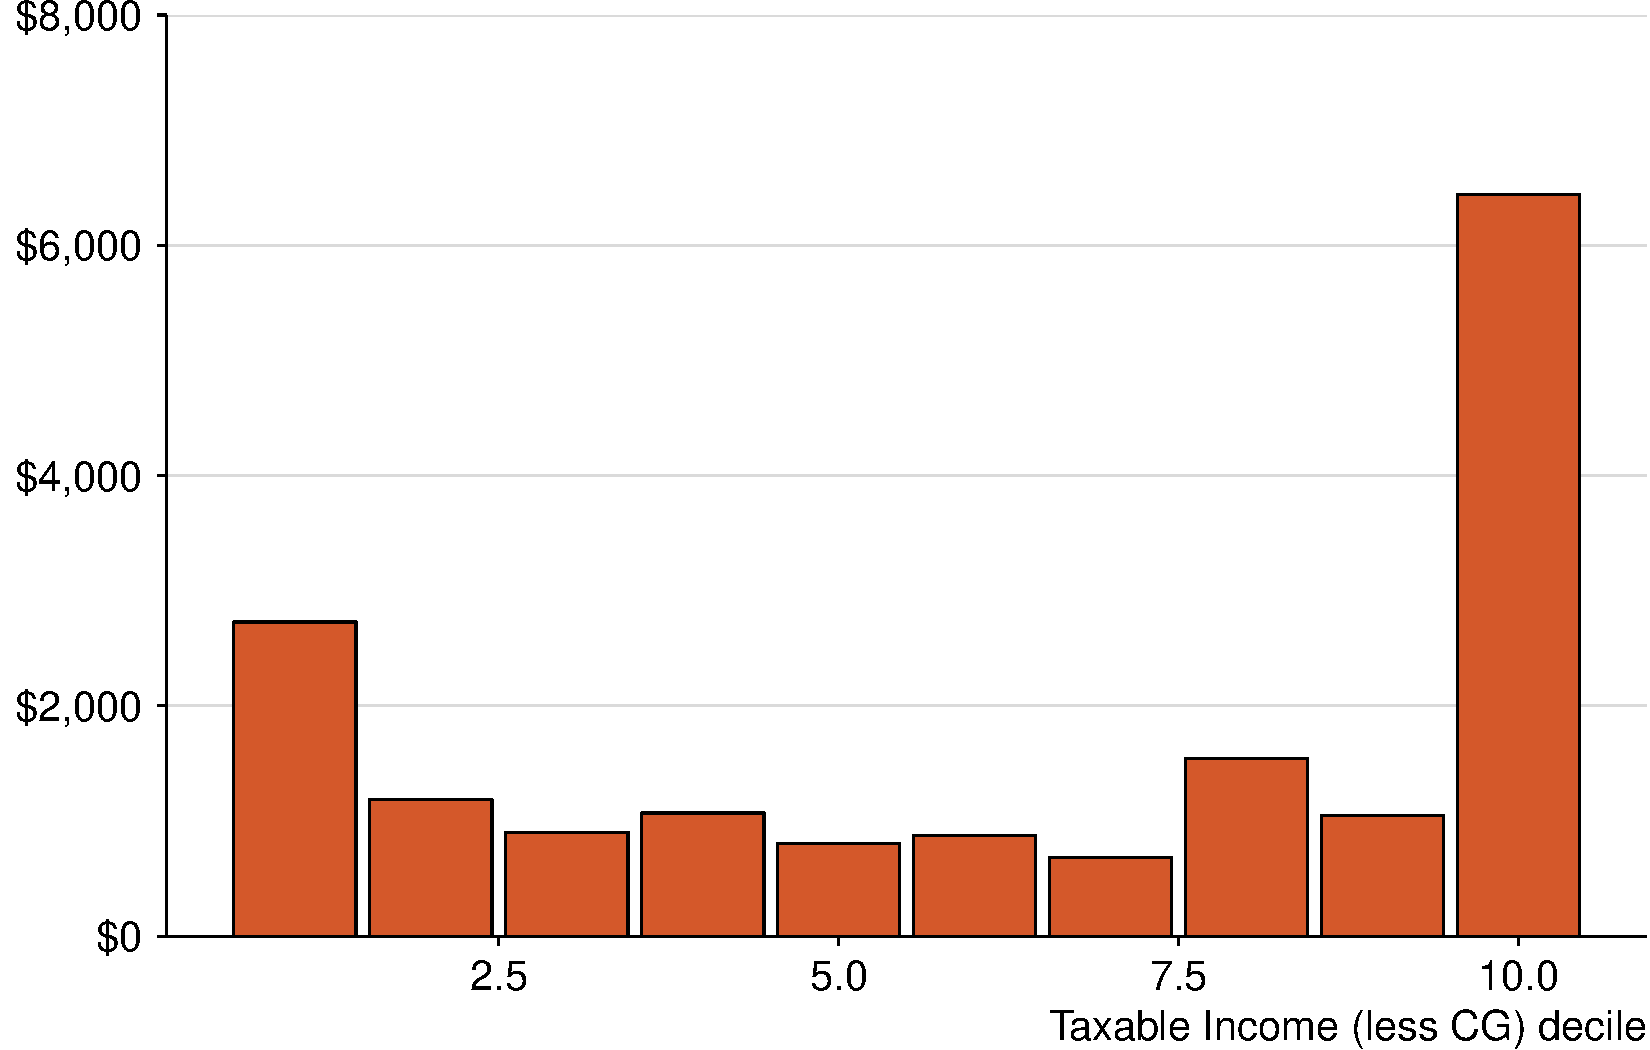
\includegraphics[width=\columnwidth]{figure/Net_capital_gains_decile_over60-1}
\notes{Net capital gains here are valued after the 50\%\ discount is applied. Deciles are calculated from the component of taxable income separate from net capital gains.}

\source{\gao\ \textcite{ATO2013i}}
\end{figure}


\begin{figure}
\Caption{Average net capital gains by income decile, taxpayers under 60}{}{fig:Net_capital_gains_under_over60}
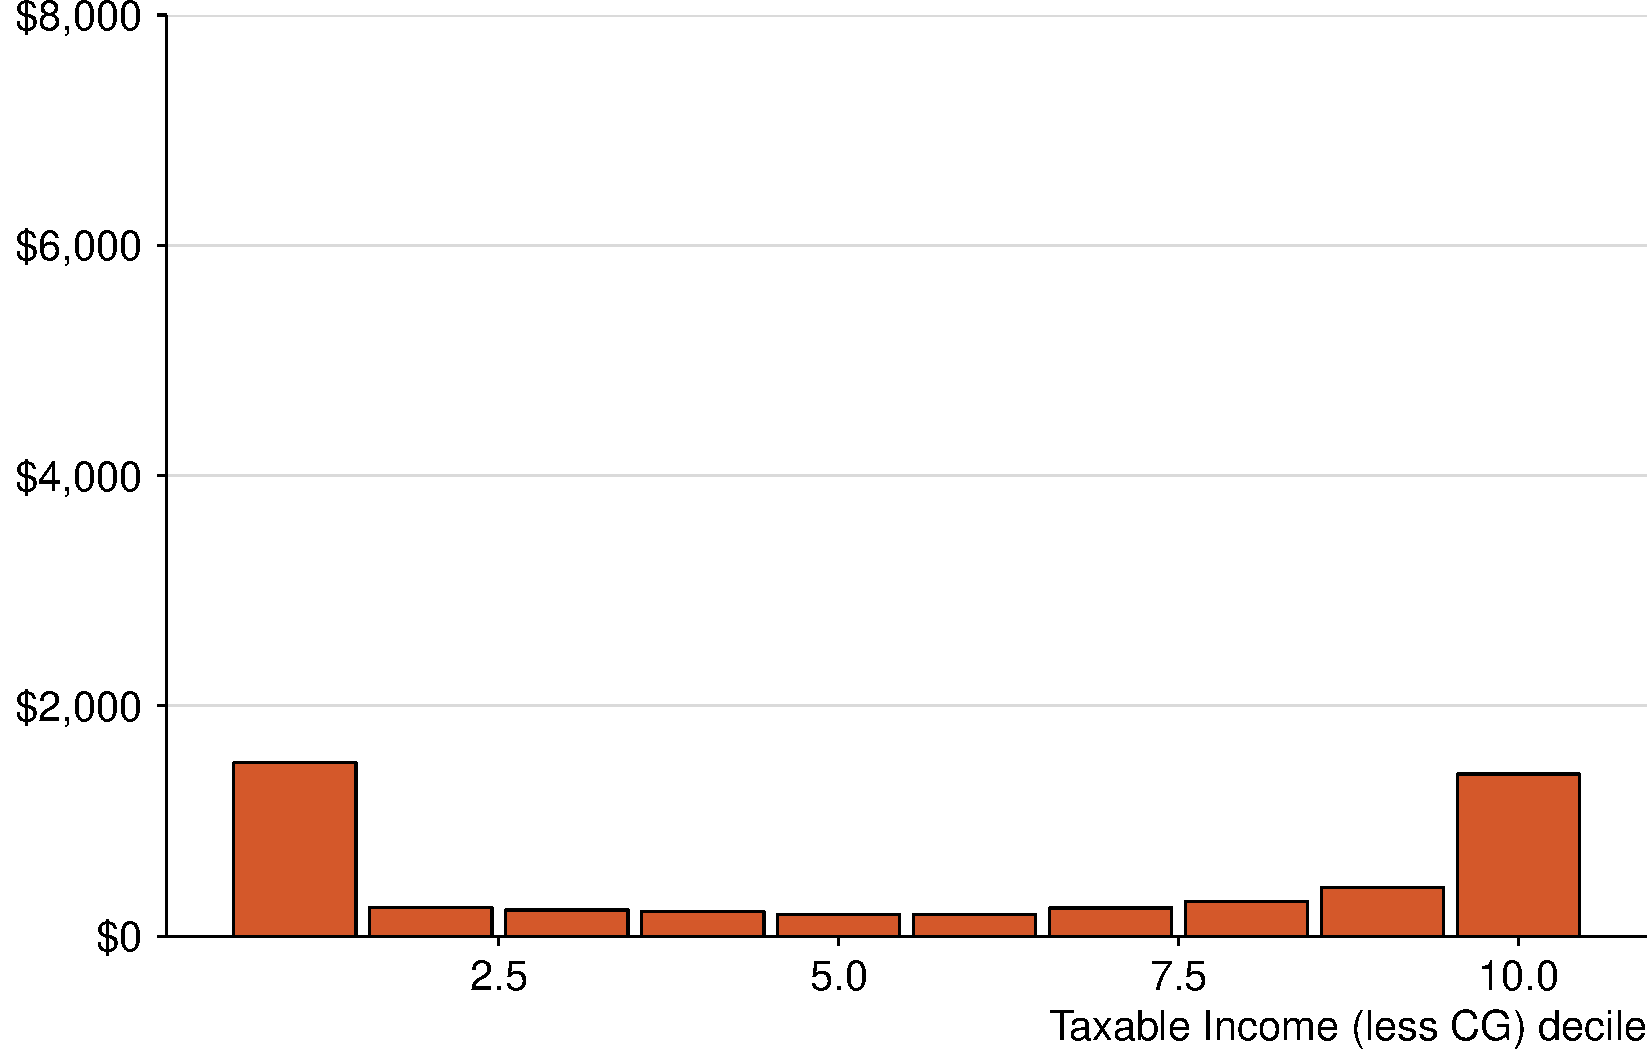
\includegraphics[width=\columnwidth]{figure/Net_capital_gains_decile_under60-1}
\notes{Net capital gains here are valued after the 50\%\ discount is applied. Deciles are calculated from the component of taxable income separate from net capital gains.}

\source{\gao\ \textcite{ATO2013i}}
\end{figure}



\chapter{Costings}
\section{Introduction}
\subsection{Technical assumptions}
The key assumptions that apply to each of the proposal costings are:
\begin{enumerate}
\item The 2012-13 2\%\ sample file obtained through \textsc{taxstats} is accurate and representative of that year.
\item The \verb=grattan::income_tax= function in the grattan R package is accurate and complete for the 2012-13 financial year.
\item The 2012-13 financial year is sufficiently representative of future years.
\end{enumerate}

\subsection{Overview of tax expenditure sanity checking}
The tax expenditure for the capital gains tax discount (E17) is \$4,180~billion.\footcite{TaxExpenditures201213} 


This differs from the amount implicit in taxstats of \$3.8~billion. The discrepancy may be the absence of benenfits to trusts in this statistic. 

\section{30\%\ CGT discount and negative gearing only for the non-salary component of taxable income}
Instead of a 50\%\ discount on the amount of capital gains that may be taxed, we propose a 30\%\ discount on the component of capital gains forming one's assessable income. Further, we propose that individuals be no longer permitted to deduct losses arising from their investments against any income other than investments and capital gains; in particular, negative gearing against salaries and wages will cease.
\subsection{Status quo}
Currently, assessable income ($I_A$) is encoded directly into tax stats
\[I_A = \verb=Taxable_Income=\]
An individual's capital gains amount is recorded in Income item 18 labels A (Net capital gains) and H (Total capital gains). Item A includes the 50\%\ discount and capital losses, but item H does not.\footnote{See \url{https://www.ato.gov.au/Individuals/Tax-Return/2013/Supplementary-tax-return/Income-questions-13-24/18---Capital-gains/}} This corresponds to items \verb=Net_CG_amt= and \verb=Tot_CY_CG_amt= respectively. We thus ignore \verb=Tot_CY_CG_amt=.

Capital gains tax for individuals is not a separate tax; it is simply a component of an individual's income tax. Once the appropriate deductions and discounts have been made, it is simply added on to a person's assessable income:
\[I_A = \text{Capital gains (after discounts, deductions)} + \text{Other income}\]
and
\[\text{tax payable} = T(I_A)\]
where $T$ is not a function of capital gains, $\frac{\partial T(\cdot)}{\partial \text{Capital gain}} = 0$.
%
\subsection{Our proposal}
We need to determine:
\begin{enumerate}
\item Total capital gains (pre-discount) for each taxpayer
\item The amount they could deduct, but can no longer
\end{enumerate}
\subsubsection{Total capital gains}
Determining total capital gains from tax stats suffers from a flaw. Only the \emph{Total capital gains} $K_T$ and the \emph{Net capital gains} $K_n$ are recorded. Net capital gains is the component of an individual's income upon which the marginal tax rate is applied -- it includes both capital losses and the capital gains discount. Total capital gains is the sum of all capital gains for the year, without capital losses or the capital gains discount.

It follows that our best estimate of the total capital gains to which the discount would apply is double the \emph{Net capital gains} amount. So the assessable income under a new regime ($I_A'$) with a discount on capital gains of $d$ will be 

\[I_A' = I_A - K_n + 2K_n(1 - d).\]

\begin{smallbox}{Tax stats}{box:TaxStatsCapitalGains}
John purchases and sells (13 months later) two houses, making capital gains of \$10,000 and \$25,000. He also experienced a capital loss of $-$\$5,000 last year which has not yet been applied against later year capital gains. His total capital gains is \$35,000 and his net capital gains is \$15,000.

In our calculations, we only see that John had a total capital gain of \$35,000 and a net capital gain of \$15,000. We infer that his total capital gains was $2\times \$15,000 = \$30,000$. 
\end{smallbox}






\subsection{Negative gearing}


\subsection{Eslake proposal: no negative gearing against salary}
Current:
\begin{align*}
I_A &= \text{Salary} + \text{Other income} \\
&\qquad{} - \text{deductions excl. rental losses} - \text{rental losses}
\end{align*}
Let:
\begin{align*}
I_S &= \text{Salary}\\
I_{A\backslash S} &= \text{Other income} \\
&\qquad{} - \text{deductions excl. rental losses} - \text{rental losses} \\
 &= I_A - I_S
\end{align*}
Then a person's assesable income under the new scenario, $I_A'$ is the person's salary where deductions are only permitted against the person's non-salary income. Deductions in excess of a person's non-salary income may not be further deducted against his salary:
\begin{align*}
I_A' &= I_S + \max\left(0, I_A - I_S \right)
\end{align*}
Note under this scenario, anyone who has a nonnegative salary \EMPH{cannot obtain a taxable loss}. Any costings using this scenario will overestimate the revenue colllectable under a scenario that violates this assumption.

\subsection{Application to taxstats}
% latex table generated in R 3.2.0 by xtable 1.7-4 package
% Mon Jun 22 15:50:05 2015
\begin{table*}[ht]
\centering
\caption{Summary table for taxable income based on $I_A' = I_S + \max(0, I_A - I_s)$.} 
\begin{tabular}{lllll}
  \hline
Net rental profit &     $I_A$ &     $I_A'$ & Tax (status quo) &   Tax (new) \\ 
  \hline
Min.   :-474901.0   & Min.   :       0   & Min.   :       0   & Min.   :      0   & Min.   :      0   \\ 
  1st Qu.:      0.0   & 1st Qu.:   21785   & 1st Qu.:   22464   & 1st Qu.:    361   & 1st Qu.:    557   \\ 
  Median :      0.0   & Median :   41561   & Median :   43178   & Median :   5301   & Median :   5875   \\ 
  Mean   :   -423.9   & Mean   :   55565   & Mean   :   57447   & Mean   :  12863   & Mean   :  13529   \\ 
  3rd Qu.:      0.0   & 3rd Qu.:   69150   & 3rd Qu.:   72111   & 3rd Qu.:  15058   & 3rd Qu.:  16065   \\ 
  Max.   : 474433.0   & Max.   :12584567   & Max.   :12584567   & Max.   :6014139   & Max.   :6014139   \\ 
   \hline
\end{tabular}
\end{table*}

So under the current regime where \$163.6~billion is payable in income tax, the above scenario renders \$172~billion payable.
\clearpage


\subsection{Time series}




\onecolumn
\section{Henry-lite proposal}
The proposal in the Henry review is to reduce both the capital gains discount and the amount one can deduct through negative gearing. In particular, the tax review proposes the discount be reduced to 30\%\ and a discount of 30\%\ be applied to both rental losses and rental income.\footnote{The income tax treatment of these household savings would be improved by applying a
40 per cent discount to most interest income, net residential rental property income, capital
gains and certain interest expenses. Doing so would provide a more consistent tax
outcome for income from bank deposits and bonds, shares, and rental properties, and
provide a means of adjusting for the effect of inflation. \textcite{Treasury2010a}.}

\begin{knitrout}
\definecolor{shadecolor}{rgb}{0.969, 0.969, 0.969}\color{fgcolor}\begin{kframe}
\begin{alltt}
\hlstd{new.discount} \hlkwb{<-} \hlnum{0.30}
\hlstd{discount_only_to_negative_rent_income} \hlkwb{<-} \hlnum{TRUE}
\end{alltt}
\end{kframe}
\end{knitrout}


\begin{knitrout}
\definecolor{shadecolor}{rgb}{0.969, 0.969, 0.969}\color{fgcolor}\begin{kframe}
\begin{alltt}
\hlkwa{if} \hlstd{(}\hlopt{!}\hlstd{discount_only_to_negative_rent_income)\{}
  \hlstd{henry_taxstats} \hlkwb{<-}
  \hlstd{taxstats201213} \hlopt
  \hlkwd{mutate}\hlstd{(}
    \hlkwc{new_capital_gains} \hlstd{=} \hlnum{2} \hlopt{*} \hlstd{Net_CG_amt} \hlopt{*} \hlstd{(}\hlnum{1} \hlopt{-} \hlstd{new.discount),}
    \hlcom{#new_net_rent = Net_rent_amt * (1 - new.discount * (Net_rent_amt < 0)),  # discount only to negative income}
    \hlkwc{new_net_rent} \hlstd{= Net_rent_amt} \hlopt{*} \hlstd{(}\hlnum{1} \hlopt{-} \hlstd{new.discount),}
    \hlkwc{new_Taxable_Income} \hlstd{= Taxable_Income} \hlopt{-} \hlstd{Net_CG_amt} \hlopt{-} \hlstd{Net_rent_amt} \hlopt{+} \hlstd{new_capital_gains} \hlopt{+} \hlstd{new_net_rent,}
    \hlkwc{current_tax} \hlstd{=} \hlkwd{income_tax}\hlstd{(Taxable_Income),}
    \hlkwc{new_tax} \hlstd{=} \hlkwd{income_tax}\hlstd{(new_Taxable_Income),}
    \hlkwc{diff} \hlstd{= new_tax} \hlopt{-} \hlstd{current_tax}
  \hlstd{)}
  \hlstd{henry_discount_remark} \hlkwb{<-} \hlstr{"in which the discount is applied to both rental income and rental losses"}
\hlstd{\}} \hlkwa{else} \hlstd{\{}
  \hlstd{henry_taxstats} \hlkwb{<-}
  \hlstd{taxstats201213} \hlopt
  \hlkwd{mutate}\hlstd{(}
    \hlkwc{new_capital_gains} \hlstd{=} \hlnum{2} \hlopt{*} \hlstd{Net_CG_amt} \hlopt{*} \hlstd{(}\hlnum{1} \hlopt{-} \hlstd{new.discount),}
    \hlkwc{new_net_rent} \hlstd{= Net_rent_amt} \hlopt{*} \hlstd{(}\hlnum{1} \hlopt{-} \hlstd{new.discount} \hlopt{*} \hlstd{(Net_rent_amt} \hlopt{<} \hlnum{0}\hlstd{)),}  \hlcom{# discount only to negative income}
    \hlcom{#new_net_rent = Net_rent_amt * (1 - new.discount),}
    \hlkwc{new_Taxable_Income} \hlstd{= Taxable_Income} \hlopt{-} \hlstd{Net_CG_amt} \hlopt{-} \hlstd{Net_rent_amt} \hlopt{+} \hlstd{new_capital_gains} \hlopt{+} \hlstd{new_net_rent,}
    \hlkwc{current_tax} \hlstd{=} \hlkwd{income_tax}\hlstd{(Taxable_Income),}
    \hlkwc{new_tax} \hlstd{=} \hlkwd{income_tax}\hlstd{(new_Taxable_Income),}
    \hlkwc{diff} \hlstd{= new_tax} \hlopt{-} \hlstd{current_tax}
  \hlstd{)}
  \hlstd{henry_discount_remark} \hlkwb{<-} \hlstr{"in which the discount is only applied to rental losses (not rental income, contra Henry)"}
\hlstd{\}}
\end{alltt}
\end{kframe}
\end{knitrout}

Under this proposal, in which the discount is only applied to rental losses (not rental income, contra Henry), income tax would rise from \$163.6~billion to \$166.3~billion.

\section{Daley (quarantining salary from losses), 30\%\ discount}
\subsection{Parameters}
\begin{knitrout}
\definecolor{shadecolor}{rgb}{0.969, 0.969, 0.969}\color{fgcolor}\begin{kframe}
\begin{alltt}
\hlstd{new.discount} \hlkwb{<-} \hlnum{0.30}
\hlstd{discount_only_to_negative_rent_income} \hlkwb{<-} \hlnum{TRUE}
\end{alltt}
\end{kframe}
\end{knitrout}

\begin{knitrout}
\definecolor{shadecolor}{rgb}{0.969, 0.969, 0.969}\color{fgcolor}\begin{kframe}
\begin{alltt}
\hlstd{daley_taxstats} \hlkwb{<-}
  \hlcom{# taxstats201213 %>%}
  \hlstd{taxstats201213} \hlopt
  \hlcom{#}
  \hlcom{# One silly entry has a CG of $25M!}
  \hlkwd{filter}\hlstd{(Net_CG_amt} \hlopt{<} \hlnum{5e6}\hlstd{)} \hlopt
  \hlkwd{mutate}\hlstd{(}
    \hlkwc{new_capital_gains} \hlstd{=} \hlnum{2} \hlopt{*} \hlstd{Net_CG_amt} \hlopt{*} \hlstd{(}\hlnum{1} \hlopt{-} \hlstd{new.discount),}
    \hlkwc{Taxable_Income_Red_CG_discount} \hlstd{= Taxable_Income} \hlopt{-} \hlstd{Net_CG_amt} \hlopt{+} \hlstd{new_capital_gains,}
    \hlcom{#}
    \hlcom{# dummy variable for following ifelse}
    \hlkwc{discount_only_to_negative_rent_income} \hlstd{= discount_only_to_negative_rent_income,}
    \hlcom{#}
    \hlkwc{new_tot_inc} \hlstd{= Tot_inc_amt} \hlopt{-} \hlstd{Net_CG_amt} \hlopt{+} \hlstd{new_capital_gains,}
    \hlkwc{income_no_salary} \hlstd{= new_tot_inc} \hlopt{-} \hlstd{Net_rent_amt} \hlopt{-} \hlstd{Sw_amt,}  \hlcom{# component of income from neither salary nor rent}
    \hlcom{#}
    \hlcom{# This is not quite true: it doesn't include medical offsets.}
    \hlcom{# You can only deduct Net_rent down to zero.  }
    \hlcom{# Include financial losses in deductions}
    \hlcom{# Full tax on Sw_amt. Then deductions}
    \hlkwc{new_Taxable_Income} \hlstd{=}  \hlkwd{pmax}\hlstd{(}\hlnum{0}\hlstd{, income_no_salary} \hlopt{+} \hlstd{Net_rent_amt} \hlopt{-} \hlstd{Net_fincl_invstmt_lss_amt)} \hlopt{+} \hlstd{Sw_amt} \hlopt{-} \hlstd{Tot_ded_amt} \hlopt{-} \hlstd{PP_loss_claimed} \hlopt{-} \hlstd{NPP_loss_claimed,}
    \hlkwc{old_Taxable_Income_no_offset} \hlstd{= Tot_inc_amt} \hlopt{-} \hlstd{Tot_ded_amt} \hlopt{-} \hlstd{PP_loss_claimed} \hlopt{-} \hlstd{NPP_loss_claimed} \hlopt{-} \hlstd{Net_fincl_invstmt_lss_amt,}
    \hlkwc{loss_ignore_CG} \hlstd{=} \hlopt{-}\hlnum{1} \hlopt{*} \hlkwd{pmin}\hlstd{(}\hlnum{0}\hlstd{,} \hlkwd{pmax}\hlstd{(}\hlnum{0}\hlstd{, income_no_salary} \hlopt{-} \hlstd{new_capital_gains)} \hlopt{+} \hlstd{Net_rent_amt),}
    \hlcom{#}
    \hlkwc{loss_carry_fwd} \hlstd{=} \hlopt{-}\hlnum{1} \hlopt{*} \hlkwd{pmin}\hlstd{(}\hlnum{0}\hlstd{, income_no_salary} \hlopt{+} \hlstd{Net_rent_amt} \hlopt{-} \hlstd{Net_fincl_invstmt_lss_amt),}
    \hlkwc{loss_carry_fwd_not_CG} \hlstd{=} \hlkwd{ifelse}\hlstd{(new_capital_gains} \hlopt{>} \hlkwd{abs}\hlstd{(Net_rent_amt)} \hlopt{&} \hlstd{Net_rent_amt} \hlopt{<} \hlnum{0}\hlstd{, Net_rent_amt,} \hlnum{0}\hlstd{),}
    \hlcom{#}
    \hlcom{# Ratio of (new?) capital gains to losses is the proportion of each taxpayer's }
    \hlcom{# capital gains that may be deducted from the rental losses which, due}
    \hlcom{# to the abolition of negative gearing in this proposal, cannot be immediately}
    \hlcom{# deducted from one's income.  The sums represent the overall ratio in the population}
    \hlcom{# which we assume to be constant year-on-year.}
    \hlcom{#}
    \hlcom{# pmin sinces can't claim more than your losses}
    \hlkwc{annualized_loss} \hlstd{=} \hlkwd{pmin}\hlstd{(}\hlnum{1}\hlstd{,} \hlkwd{abs}\hlstd{(}\hlkwd{sum}\hlstd{(new_capital_gains)} \hlopt{/} \hlkwd{sum}\hlstd{(loss_carry_fwd)))} \hlopt{*} \hlstd{loss_carry_fwd,}  \hlcom{# nonnegative}
    \hlcom{#}
    \hlcom{# The consequence of the following calc is that some new_Taxable_Income_post_carryfwd will be NEGATIVE }
    \hlcom{# -- i.e. unexhausted (especially if the Taxable_Income (originally) was zero).  This error will}
    \hlcom{# overestimate the amount of extra tax collected.  However}
    \hlcom{#}
    \hlcom{#   daley_taxstats %>% }
    \hlcom{#     filter(new_Taxable_Income_post_carryfwd < 0) %$% sum(new_Taxable_Income) * 50 / 1e9}
    \hlcom{#   # [1] 0.224  # 224 million in losses}
    \hlcom{#}
    \hlcom{# i.e. There are at most 224 million dollars in losses carried forward that are unaccounted for}
    \hlcom{# in this model.  And so at most 224 * 0.485 = 109 million in taxable income AT MOST that is }
    \hlcom{# possibly lost. My doona is comfy: I'm staying in bed for that.}
    \hlkwc{new_Taxable_Income_post_carryfwd} \hlstd{= new_Taxable_Income} \hlopt{-} \hlstd{annualized_loss,}  \hlcom{# remembering ann.lss is nonnegative}
    \hlkwc{current_tax} \hlstd{=} \hlkwd{income_tax}\hlstd{(old_Taxable_Income_no_offset),}
    \hlkwc{tax_after_reduction_in_discount} \hlstd{=} \hlkwd{income_tax}\hlstd{(Taxable_Income_Red_CG_discount),}
    \hlkwc{new_tax} \hlstd{=} \hlkwd{income_tax}\hlstd{(new_Taxable_Income),}
    \hlkwc{diff} \hlstd{= new_tax} \hlopt{-} \hlstd{current_tax,}
    \hlkwc{diff_incl_carry_fwd} \hlstd{=} \hlkwd{income_tax}\hlstd{(new_Taxable_Income_post_carryfwd)} \hlopt{-} \hlstd{current_tax}
  \hlstd{)}

\hlkwa{if} \hlstd{(discount_only_to_negative_rent_income)\{}
  \hlstd{daley_discount_remark} \hlkwb{<-} \hlstr{"in which the discount is only applied to rental losses (not rental income, contra Henry)"}
\hlstd{\}} \hlkwa{else} \hlstd{\{}
  \hlstd{daley_discount_remark} \hlkwb{<-} \hlstr{"in which the discount is applied to both rental income and rental losses"}
\hlstd{\}}
\end{alltt}
\end{kframe}
\end{knitrout}
Under this proposal, income tax would rise from \$163.1~billion to \$167.4~billion. (2012-13 taxstats) But the extra revenue due to this policy will reduce: losses brought forward (that would have otherwise been used to reduce ordinary taxable income) will be offset against capital gains. This will reduce the increased revenue for \$4.4~bn to \$1.4~bn.
%
\subsection{Pushing forward the losses}
\subsubsection{Infer by age}
\paragraph{Age}
\begin{knitrout}
\definecolor{shadecolor}{rgb}{0.969, 0.969, 0.969}\color{fgcolor}\begin{kframe}
\begin{alltt}
\hlstd{daley_taxstats_with_age} \hlkwb{<-}
  \hlstd{daley_taxstats} \hlopt
  \hlcom{# random}
  \hlkwd{mutate}\hlstd{(}\hlkwc{age_imp} \hlstd{=} \hlkwd{floor}\hlstd{(}\hlnum{17.5} \hlopt{+} \hlnum{5} \hlopt{*} \hlstd{(}\hlnum{11} \hlopt{-} \hlstd{age_range)} \hlopt{+} \hlkwd{runif}\hlstd{(}\hlkwd{nrow}\hlstd{(.),} \hlopt{-}\hlnum{2.5}\hlstd{,} \hlnum{2.5}\hlstd{)))} \hlopt
  \hlkwd{mutate}\hlstd{(}\hlkwc{loss_carry_fwd_orig} \hlstd{= loss_carry_fwd)}

\hlstd{prob_of_CG_event_by_age} \hlkwb{<-}
  \hlstd{daley_taxstats_with_age} \hlopt
  \hlkwd{group_by}\hlstd{(age_imp)} \hlopt
  \hlkwd{summarise}\hlstd{(}\hlkwc{CG_event_prob} \hlstd{=} \hlkwd{mean}\hlstd{(new_capital_gains} \hlopt{>} \hlnum{0}\hlstd{))}

\hlstd{size_of_CG_event} \hlkwb{<-}
  \hlstd{daley_taxstats_with_age} \hlopt
  \hlkwd{filter}\hlstd{(new_capital_gains} \hlopt{>} \hlnum{0}\hlstd{)} \hlopt
  \hlkwd{group_by}\hlstd{(age_imp)} \hlopt
  \hlkwd{summarise}\hlstd{(}\hlkwc{size_of_hypoth_CG} \hlstd{=} \hlkwd{mean}\hlstd{(new_capital_gains))}

\hlstd{losses_by_age} \hlkwb{<-}
  \hlstd{daley_taxstats_with_age} \hlopt
  \hlkwd{group_by}\hlstd{(age_imp)} \hlopt
  \hlkwd{summarise}\hlstd{(}\hlkwc{avg_loss_carried_fwd} \hlstd{=} \hlkwd{mean}\hlstd{(loss_ignore_CG))}

\hlstd{taxable_income_by_age} \hlkwb{<-}
  \hlstd{daley_taxstats_with_age} \hlopt
  \hlkwd{group_by}\hlstd{(age_imp)} \hlopt
  \hlkwd{summarise}\hlstd{(}\hlkwc{avg.taxable_income} \hlstd{=} \hlkwd{mean}\hlstd{(Taxable_Income))}
\end{alltt}
\end{kframe}
\end{knitrout}

\begin{knitrout}
\definecolor{shadecolor}{rgb}{0.969, 0.969, 0.969}\color{fgcolor}\begin{kframe}
\begin{alltt}
\hlstd{capital_gains_by_losses4} \hlkwb{<-}
  \hlstd{daley_taxstats} \hlopt
  \hlkwd{group_by}\hlstd{(}\hlkwc{IsInvestor} \hlstd{= Gross_rent_amt} \hlopt{>} \hlnum{0}\hlstd{,}
           \hlkwc{HasLoss} \hlstd{= loss_ignore_CG} \hlopt{>} \hlnum{0}\hlstd{,}
           \hlkwc{HasCG} \hlstd{= new_capital_gains} \hlopt{>} \hlnum{0}\hlstd{)} \hlopt
  \hlstd{tally} \hlopt
  \hlkwd{arrange}\hlstd{(IsInvestor, HasLoss, HasCG)} \hlopt
  \hlcom{#}
  \hlcom{# cosmetics:}
  \hlstd{ungroup} \hlopt
  \hlkwd{group_by}\hlstd{(IsInvestor)} \hlopt
  \hlkwd{mutate}\hlstd{(}\hlkwc{prop} \hlstd{=} \hlkwd{round}\hlstd{(n}\hlopt{/}\hlkwd{sum}\hlstd{(n),}\hlnum{3}\hlstd{))}
\hlcom{# Source: local data table [8 x 5]}
\hlcom{# }
\hlcom{#   IsInvestor HasLoss HasCG      n  prop}
\hlcom{# 1      FALSE   FALSE FALSE 208423 0.968}
\hlcom{# 2      FALSE   FALSE  TRUE   6656 0.031}
\hlcom{# 3      FALSE    TRUE FALSE    256 0.001}
\hlcom{# 4      FALSE    TRUE  TRUE     23 0.000}
\hlcom{#--}
\hlcom{# 5       TRUE   FALSE FALSE  20753 0.533}
\hlcom{# 6       TRUE   FALSE  TRUE   2340 0.060}
\hlcom{# 7       TRUE    TRUE FALSE  14724 0.378}
\hlcom{# 8       TRUE    TRUE  TRUE   1143 0.029}

\hlstd{new_daley} \hlkwb{<-}
  \hlstd{daley_taxstats} \hlopt
  \hlcom{# random}
  \hlkwd{mutate}\hlstd{(}\hlkwc{age_imp} \hlstd{=} \hlkwd{floor}\hlstd{(}\hlnum{17.5} \hlopt{+} \hlnum{5} \hlopt{*} \hlstd{(}\hlnum{11}\hlopt{-}\hlstd{age_range)} \hlopt{+} \hlkwd{runif}\hlstd{(}\hlkwd{nrow}\hlstd{(.),} \hlopt{-}\hlnum{2.5}\hlstd{,} \hlnum{2.5}\hlstd{)))} \hlopt
  \hlkwd{mutate}\hlstd{(}\hlkwc{loss_carry_fwd_orig} \hlstd{= loss_ignore_CG)} \hlopt
  \hlkwd{merge}\hlstd{(size_of_CG_event,} \hlkwc{by} \hlstd{=} \hlstr{"age_imp"}\hlstd{)} \hlopt
  \hlkwd{mutate}\hlstd{(}\hlkwc{hasHadCG} \hlstd{=} \hlnum{FALSE}\hlstd{,}  \hlcom{#yet}
         \hlkwc{whenCG.lastoccurred} \hlstd{=} \hlnum{0}\hlstd{,}
         \hlkwc{prev_unexhausted_loss} \hlstd{= loss_ignore_CG)}

\hlkwa{for} \hlstd{(i} \hlkwa{in} \hlnum{1}\hlopt{:}\hlnum{20}\hlstd{)\{}
\hlkwd{gc}\hlstd{()}
\hlstd{new_daley} \hlopt
    \hlkwd{select}\hlstd{(age_imp, loss_carry_fwd_orig, prev_unexhausted_loss,}
           \hlstd{whenCG.lastoccurred, size_of_hypoth_CG,}
           \hlstd{hasHadCG,}
           \hlstd{new_Taxable_Income, current_tax)} \hlopt
    \hlkwd{mutate}\hlstd{(}\hlkwc{rand} \hlstd{=} \hlkwd{runif}\hlstd{(}\hlkwd{nrow}\hlstd{(.)))} \hlopt
    \hlkwd{mutate}\hlstd{(}\hlkwc{noCGevent} \hlstd{= rand} \hlopt{<} \hlnum{0.533} \hlopt{+} \hlnum{0.378}\hlstd{)} \hlopt  \hlcom{# approx 90% # v.s. table}
    \hlkwd{mutate}\hlstd{(}
      \hlkwc{loss_carry_fwd} \hlstd{=} \hlkwd{ifelse}\hlstd{(noCGevent,}
                              \hlstd{loss_carry_fwd_orig} \hlopt{*} \hlstd{i,}  \hlcom{#unimportant}
                              \hlcom{#}
                              \hlcom{# if they do have a capital gains event, we}
                              \hlcom{# estimate the size of the CG event by the average }
                              \hlcom{# for their age (in the groundhog year).  The losses have}
                              \hlcom{# accumulated over time: previously unexhuasted losses from}
                              \hlcom{# previous CG events where this hasn't been zero.  And the }
                              \hlcom{# losses built up from the first year of the new policy. }
                              \hlkwd{pmax}\hlstd{(}\hlnum{0}\hlstd{, prev_unexhausted_loss} \hlopt{+}
                                       \hlstd{loss_carry_fwd_orig} \hlopt{*} \hlstd{(i} \hlopt{-} \hlnum{1} \hlopt{-} \hlstd{whenCG.lastoccurred)} \hlopt{-}
                                       \hlstd{size_of_hypoth_CG)),}
      \hlcom{# }
      \hlkwc{wasCompleteLoss} \hlstd{=} \hlopt{!}\hlstd{noCGevent} \hlopt{&} \hlstd{loss_carry_fwd_orig} \hlopt{*} \hlstd{(i} \hlopt{-} \hlstd{whenCG.lastoccurred)} \hlopt{-} \hlstd{size_of_hypoth_CG} \hlopt{<=} \hlnum{0}\hlstd{,}

      \hlkwc{now_Taxable_Income} \hlstd{=} \hlkwd{ifelse}\hlstd{(noCGevent,}
                                  \hlstd{new_Taxable_Income,}
                                  \hlkwd{pmax}\hlstd{(}\hlnum{0}\hlstd{, new_Taxable_Income} \hlopt{-} \hlstd{loss_carry_fwd)),}
      \hlcom{# Here we assume CG in CG event year is zero to provide an upper bound of losses.}
      \hlkwc{now_Taxable_Income2} \hlstd{=} \hlkwd{ifelse}\hlstd{(noCGevent,}
                                   \hlstd{new_Taxable_Income,}
                                   \hlkwd{pmax}\hlstd{(}\hlnum{0}\hlstd{, new_Taxable_Income} \hlopt{-}
                                          \hlstd{loss_carry_fwd_orig} \hlopt{*} \hlstd{(i} \hlopt{-} \hlstd{whenCG.lastoccurred))),}
      \hlkwc{new_tax} \hlstd{=} \hlkwd{income_tax}\hlstd{(now_Taxable_Income),}
      \hlkwc{new_tax2}\hlstd{=} \hlkwd{income_tax}\hlstd{(now_Taxable_Income2),}
      \hlkwc{diff} \hlstd{= new_tax} \hlopt{-} \hlstd{current_tax,}
      \hlkwc{diff2} \hlstd{= new_tax2} \hlopt{-} \hlstd{current_tax,}
      \hlcom{#}
      \hlcom{# retrospective variables}
      \hlkwc{prev_unexhausted_loss} \hlstd{=} \hlkwd{ifelse}\hlstd{(noCGevent,}
                                     \hlstd{prev_unexhausted_loss,}
                                     \hlkwd{pmax}\hlstd{(}\hlnum{0}\hlstd{, loss_carry_fwd_orig} \hlopt{*} \hlstd{(i} \hlopt{-} \hlstd{whenCG.lastoccurred)} \hlopt{-}
                                            \hlstd{size_of_hypoth_CG)}
      \hlstd{),}
      \hlkwc{loss_still_available} \hlstd{=} \hlkwd{pmax}\hlstd{(}\hlnum{0}\hlstd{, loss_carry_fwd_orig} \hlopt{*} \hlstd{(i} \hlopt{-} \hlstd{whenCG.lastoccurred)} \hlopt{-} \hlstd{size_of_hypoth_CG),}
      \hlkwc{whenCG.lastoccurred} \hlstd{=} \hlkwd{ifelse}\hlstd{(}\hlopt{!}\hlstd{noCGevent, i, whenCG.lastoccurred),}
      \hlkwc{hasHadCG} \hlstd{=} \hlkwd{as.logical}\hlstd{(}\hlkwd{pmax}\hlstd{(hasHadCG} \hlopt{+ !}\hlstd{noCGevent,} \hlnum{1}\hlstd{))}  \hlcom{# unimportant}
    \hlstd{)} \hlopt
    \hlstd{data.table}

  \hlkwa{if} \hlstd{(i} \hlopt \hlnum{5} \hlopt{==} \hlnum{0} \hlopt{||} \hlstd{i} \hlopt{==} \hlnum{1}\hlstd{)\{}
    \hlkwd{cat}\hlstd{(}\hlstr{"Year"}\hlstd{, i,} \hlstr{"New income:\textbackslash{}n"}\hlstd{,}  \hlkwd{paste0}\hlstd{(}\hlstr{"$"}\hlstd{,} \hlkwd{round}\hlstd{(}\hlkwd{sum}\hlstd{(new_daley}\hlopt{$}\hlstd{diff)}\hlopt{*}\hlnum{50}\hlopt{/}\hlnum{1e9}\hlstd{,} \hlnum{1}\hlstd{)),} \hlstr{"bn\textbackslash{}n"}\hlstd{,}
        \hlstr{"New income2:\textbackslash{}n"}\hlstd{,}  \hlkwd{paste0}\hlstd{(}\hlstr{"$"}\hlstd{,} \hlkwd{round}\hlstd{(}\hlkwd{sum}\hlstd{(new_daley}\hlopt{$}\hlstd{diff2)}\hlopt{*}\hlnum{50}\hlopt{/}\hlnum{1e9}\hlstd{,} \hlnum{1}\hlstd{)),} \hlstr{"bn\textbackslash{}n\textbackslash{}n"}\hlstd{)}
  \hlstd{\}}
\hlstd{\}}
\end{alltt}
\begin{verbatim}
## Year 1 New income:
##  $4.3 bn
##  New income2:
##  $4.1 bn
## 
## Year 5 New income:
##  $3.9 bn
##  New income2:
##  $3.7 bn
## 
## Year 10 New income:
##  $3.7 bn
##  New income2:
##  $3.6 bn
## 
## Year 15 New income:
##  $3.6 bn
##  New income2:
##  $3.6 bn
## 
## Year 20 New income:
##  $3.6 bn
##  New income2:
##  $3.6 bn
\end{verbatim}
\end{kframe}
\end{knitrout}
Under these assumptions, the effect of the tax reduces from \$4.4~billion to \$3.6~billion after 20~years.


\begin{table*}
\Caption{Costings for the two policies}{Using the 2012-13 sample file, contemporaneous dollars}{tbl:Costings}
\begin{tabular}{lrrr}
 & & Initial change in revenue & Eventual change \\
 \hline
 Henry lite & & \$2.7~bn & \$2.7~bn\\[4pt]
 Quarantine losses from salary & Simple & \$4.4~bn & \$1.4~bn \\
                            & Secondary & \$4.4~bn & \$3.6~bn
\end{tabular}
\end{table*}


\chapter{Dani's presentation numbers}
\onecolumn
\section{Reduce CGT discount and limit negative gearing}
\begin{knitrout}
\definecolor{shadecolor}{rgb}{0.969, 0.969, 0.969}\color{fgcolor}\begin{kframe}
\begin{alltt}
\hlstd{new.discount} \hlkwb{<-} \hlnum{0.3}

\hlstd{taxstats201213} \hlopt
  \hlcom{# Reduce CGT discount to 30%}
  \hlkwd{mutate}\hlstd{(}
    \hlkwc{new_capital_gains} \hlstd{=} \hlnum{2} \hlopt{*} \hlstd{Net_CG_amt} \hlopt{*} \hlstd{(}\hlnum{1} \hlopt{-} \hlstd{new.discount),}
    \hlkwc{Taxable_Income_No_CG_discount} \hlstd{= Taxable_Income} \hlopt{-} \hlstd{Net_CG_amt} \hlopt{+} \hlstd{new_capital_gains,}
    \hlcom{## is this right? -- BC: Glanced and corrected Net_rent_amt sign.}
    \hlkwc{Taxable_Income_new_proposal} \hlstd{=} \hlkwd{ifelse}\hlstd{(Net_rent_amt} \hlopt{<} \hlnum{0}\hlstd{,}
                                         \hlkwd{pmax}\hlstd{(}\hlnum{0}\hlstd{, Taxable_Income_No_CG_discount} \hlopt{-} \hlstd{Sw_amt} \hlopt{+} \hlstd{Net_rent_amt)} \hlopt{+} \hlstd{Sw_amt,}
                                         \hlstd{Taxable_Income_No_CG_discount),}
    \hlkwc{loss_carry_fwd} \hlstd{=} \hlkwd{pmin}\hlstd{(}\hlnum{0}\hlstd{,Taxable_Income_No_CG_discount} \hlopt{-} \hlstd{Sw_amt} \hlopt{+} \hlstd{Net_rent_amt),}
    \hlkwc{current_tax} \hlstd{=} \hlkwd{income_tax}\hlstd{(Taxable_Income),}
    \hlkwc{new_tax} \hlstd{=} \hlkwd{income_tax}\hlstd{(Taxable_Income_new_proposal),}
    \hlkwc{new_tax_with_carry_fwd} \hlstd{=} \hlkwd{income_tax}\hlstd{(Taxable_Income_new_proposal} \hlopt{+} \hlstd{loss_carry_fwd),}
    \hlkwc{diff} \hlstd{= new_tax} \hlopt{-} \hlstd{current_tax}
  \hlstd{)} \hlopt
  \hlkwd{sum}\hlstd{(diff)} \hlopt{*} \hlnum{50} \hlopt{/} \hlnum{1e9} \hlkwb{->}
  \hlstd{reduce_cgt_limit_negative_gearing_costing}

\hlkwd{print}\hlstd{(reduce_cgt_limit_negative_gearing_costing)}
\end{alltt}
\begin{verbatim}
## [1] 4.170514
\end{verbatim}
\end{kframe}
\end{knitrout}


\begin{knitrout}
\definecolor{shadecolor}{rgb}{0.969, 0.969, 0.969}\color{fgcolor}\begin{kframe}
\begin{alltt}
\hlstd{new.discount} \hlkwb{<-} \hlnum{0.3}

\hlkwd{fread}\hlstd{(}\hlstr{"2012 2% individuals sample file.csv"}\hlstd{)} \hlopt
  \hlcom{# Reduce CGT discount to 30%}
  \hlkwd{mutate}\hlstd{(}
    \hlkwc{new_capital_gains} \hlstd{=} \hlnum{2} \hlopt{*} \hlstd{Net_CG_amt} \hlopt{*} \hlstd{(}\hlnum{1} \hlopt{-} \hlstd{new.discount),}
    \hlkwc{Taxable_Income_No_CG_discount} \hlstd{= Taxable_Income} \hlopt{-} \hlstd{Net_CG_amt} \hlopt{+} \hlstd{new_capital_gains,}
    \hlcom{## is this right? -- BC: Glanced and corrected Net_rent_amt sign.}
    \hlkwc{Taxable_Income_new_proposal} \hlstd{=} \hlkwd{ifelse}\hlstd{(Net_rent_amt} \hlopt{<} \hlnum{0}\hlstd{,}
                                         \hlkwd{pmax}\hlstd{(}\hlnum{0}\hlstd{, Taxable_Income_No_CG_discount} \hlopt{-} \hlstd{Sw_amt} \hlopt{+} \hlstd{Net_rent_amt)} \hlopt{+} \hlstd{Sw_amt,}
                                         \hlstd{Taxable_Income_No_CG_discount),}
    \hlkwc{loss_carry_fwd} \hlstd{=} \hlkwd{pmin}\hlstd{(}\hlnum{0}\hlstd{,Taxable_Income_No_CG_discount} \hlopt{-} \hlstd{Sw_amt} \hlopt{+} \hlstd{Net_rent_amt),}
    \hlkwc{current_tax} \hlstd{=} \hlkwd{income_tax}\hlstd{(Taxable_Income,} \hlkwc{fy.year} \hlstd{=} \hlstr{"2011-12"}\hlstd{),}
    \hlkwc{new_tax} \hlstd{=} \hlkwd{income_tax}\hlstd{(Taxable_Income_new_proposal,} \hlkwc{fy.year} \hlstd{=} \hlstr{"2011-12"}\hlstd{),}
    \hlkwc{diff} \hlstd{= new_tax} \hlopt{-} \hlstd{current_tax}
  \hlstd{)} \hlopt
  \hlkwd{sum}\hlstd{(diff)} \hlopt{*} \hlnum{50} \hlopt{/} \hlnum{1e9} \hlkwb{->}
  \hlstd{reduce_cgt_limit_negative_gearing_costing_1112}

\hlkwd{print}\hlstd{(reduce_cgt_limit_negative_gearing_costing_1112)}
\end{alltt}
\begin{verbatim}
## [1] 4.233905
\end{verbatim}
\end{kframe}
\end{knitrout}
\section{Daley discount}

\section{Daley (30\%\ symmetrical discount)}
\begin{knitrout}
\definecolor{shadecolor}{rgb}{0.969, 0.969, 0.969}\color{fgcolor}\begin{kframe}
\begin{alltt}
\hlstd{new.discount} \hlkwb{<-} \hlnum{0.3}

\hlstd{discount_only_to_negative_rent_income} \hlkwb{<-} \hlnum{FALSE}

\hlkwa{if} \hlstd{(discount_only_to_negative_rent_income)\{}
  \hlstd{daley_taxstats} \hlkwb{<-}
  \hlstd{taxstats201213} \hlopt
  \hlkwd{mutate}\hlstd{(}
    \hlkwc{new_capital_gains} \hlstd{=} \hlnum{2} \hlopt{*} \hlstd{Net_CG_amt} \hlopt{*} \hlstd{(}\hlnum{1} \hlopt{-} \hlstd{new.discount),}
    \hlkwc{new_net_rent} \hlstd{= Net_rent_amt} \hlopt{*} \hlstd{(}\hlnum{1} \hlopt{-} \hlstd{new.discount} \hlopt{*} \hlstd{(Net_rent_amt} \hlopt{<} \hlnum{0}\hlstd{)),}  \hlcom{# discount only to negative income}
    \hlcom{#new_net_rent = Net_rent_amt * (1 - new.discount),}
    \hlkwc{new_Taxable_Income} \hlstd{= Taxable_Income} \hlopt{-} \hlstd{Net_CG_amt} \hlopt{-} \hlstd{Net_rent_amt} \hlopt{+} \hlstd{new_capital_gains} \hlopt{+} \hlstd{new_net_rent,}
    \hlkwc{current_tax} \hlstd{=} \hlkwd{income_tax}\hlstd{(Taxable_Income),}
    \hlkwc{new_tax} \hlstd{=} \hlkwd{income_tax}\hlstd{(new_Taxable_Income),}
    \hlkwc{diff} \hlstd{= new_tax} \hlopt{-} \hlstd{current_tax}
  \hlstd{)}
  \hlstd{daley_discount_remark} \hlkwb{<-} \hlstr{"in which the discount is only applied to rental losses (not rental income, contra Henry)"}
\hlstd{\}} \hlkwa{else} \hlstd{\{}
  \hlstd{daley_taxstats} \hlkwb{<-}
  \hlstd{taxstats201213} \hlopt
  \hlkwd{mutate}\hlstd{(}
    \hlkwc{new_capital_gains} \hlstd{=} \hlnum{2} \hlopt{*} \hlstd{Net_CG_amt} \hlopt{*} \hlstd{(}\hlnum{1} \hlopt{-} \hlstd{new.discount),}
    \hlcom{#new_net_rent = Net_rent_amt * (1 - new.discount * (Net_rent_amt < 0)),  # discount only to negative income}
    \hlkwc{new_net_rent} \hlstd{= Net_rent_amt} \hlopt{*} \hlstd{(}\hlnum{1} \hlopt{-} \hlstd{new.discount),}
    \hlkwc{new_Taxable_Income} \hlstd{= Taxable_Income} \hlopt{-} \hlstd{Net_CG_amt} \hlopt{-} \hlstd{Net_rent_amt} \hlopt{+} \hlstd{new_capital_gains} \hlopt{+} \hlstd{new_net_rent,}
    \hlkwc{current_tax} \hlstd{=} \hlkwd{income_tax}\hlstd{(Taxable_Income),}
    \hlkwc{new_tax} \hlstd{=} \hlkwd{income_tax}\hlstd{(new_Taxable_Income),}
    \hlkwc{diff} \hlstd{= new_tax} \hlopt{-} \hlstd{current_tax}
  \hlstd{)}
  \hlstd{daley_discount_remark} \hlkwb{<-} \hlstr{"in which the discount is applied to both rental income and rental losses"}
\hlstd{\}}
\end{alltt}
\end{kframe}
\end{knitrout}

\begin{knitrout}
\definecolor{shadecolor}{rgb}{0.969, 0.969, 0.969}\color{fgcolor}\begin{kframe}
\begin{alltt}
\hlstd{new.discount} \hlkwb{<-} \hlnum{0.3}

\hlstd{discount_only_to_negative_rent_income} \hlkwb{<-} \hlnum{FALSE}

\hlkwa{if} \hlstd{(discount_only_to_negative_rent_income)\{}
  \hlstd{daley_taxstats_1112} \hlkwb{<-}
  \hlkwd{fread}\hlstd{(}\hlstr{"2012 2% individuals sample file.csv"}\hlstd{)} \hlopt
  \hlkwd{mutate}\hlstd{(}
    \hlkwc{new_capital_gains} \hlstd{=} \hlnum{2} \hlopt{*} \hlstd{Net_CG_amt} \hlopt{*} \hlstd{(}\hlnum{1} \hlopt{-} \hlstd{new.discount),}
    \hlkwc{new_net_rent} \hlstd{= Net_rent_amt} \hlopt{*} \hlstd{(}\hlnum{1} \hlopt{-} \hlstd{new.discount} \hlopt{*} \hlstd{(Net_rent_amt} \hlopt{<} \hlnum{0}\hlstd{)),}  \hlcom{# discount only to negative income}
    \hlcom{#new_net_rent = Net_rent_amt * (1 - new.discount),}
    \hlkwc{new_Taxable_Income} \hlstd{= Taxable_Income} \hlopt{-} \hlstd{Net_CG_amt} \hlopt{-} \hlstd{Net_rent_amt} \hlopt{+} \hlstd{new_capital_gains} \hlopt{+} \hlstd{new_net_rent,}
    \hlkwc{current_tax} \hlstd{=} \hlkwd{income_tax}\hlstd{(Taxable_Income,} \hlkwc{fy.year} \hlstd{=} \hlstr{"2011-12"}\hlstd{),}
    \hlkwc{new_tax} \hlstd{=} \hlkwd{income_tax}\hlstd{(new_Taxable_Income,} \hlkwc{fy.year} \hlstd{=} \hlstr{"2011-12"}\hlstd{),}
    \hlkwc{diff} \hlstd{= new_tax} \hlopt{-} \hlstd{current_tax}
  \hlstd{)}
  \hlstd{daley_discount_remark_1112} \hlkwb{<-} \hlstr{"in which the discount is only applied to rental losses (not rental income, contra Henry)"}
\hlstd{\}} \hlkwa{else} \hlstd{\{}
  \hlstd{daley_taxstats_1112} \hlkwb{<-}
  \hlkwd{fread}\hlstd{(}\hlstr{"2012 2% individuals sample file.csv"}\hlstd{)} \hlopt
  \hlkwd{mutate}\hlstd{(}
    \hlkwc{new_capital_gains} \hlstd{=} \hlnum{2} \hlopt{*} \hlstd{Net_CG_amt} \hlopt{*} \hlstd{(}\hlnum{1} \hlopt{-} \hlstd{new.discount),}
    \hlcom{#new_net_rent = Net_rent_amt * (1 - new.discount * (Net_rent_amt < 0)),  # discount only to negative income}
    \hlkwc{new_net_rent} \hlstd{= Net_rent_amt} \hlopt{*} \hlstd{(}\hlnum{1} \hlopt{-} \hlstd{new.discount),}
    \hlkwc{new_Taxable_Income} \hlstd{= Taxable_Income} \hlopt{-} \hlstd{Net_CG_amt} \hlopt{-} \hlstd{Net_rent_amt} \hlopt{+} \hlstd{new_capital_gains} \hlopt{+} \hlstd{new_net_rent,}
    \hlkwc{current_tax} \hlstd{=} \hlkwd{income_tax}\hlstd{(Taxable_Income,} \hlkwc{fy.year} \hlstd{=} \hlstr{"2011-12"}\hlstd{),}
    \hlkwc{new_tax} \hlstd{=} \hlkwd{income_tax}\hlstd{(new_Taxable_Income,} \hlkwc{fy.year} \hlstd{=} \hlstr{"2011-12"}\hlstd{),}
    \hlkwc{diff} \hlstd{= new_tax} \hlopt{-} \hlstd{current_tax}
  \hlstd{)}
  \hlstd{daley_discount_remark_1112} \hlkwb{<-} \hlstr{"in which the discount is applied to both rental income and rental losses"}
\hlstd{\}}
\end{alltt}
\end{kframe}
\end{knitrout}
Under this proposal, income tax would rise from \$163.6~billion to \$165.7~billion. 

\section{Summary}
\begin{table*}
\centering
\caption{Summary of costings}
\begin{tabular}{lrrp{5.1cm}}
 & 2011-12 & 2012-13 & \\
Reduce CGT and limit negative gearing & \$4~billion & \$4.2~billion&\\
Daley symmetric 30\%\ discount & \$2.1~billion & \$2.1~billion&\emph{in which the discount is applied to both rental income and rental losses}
\end{tabular}

\notes{Contemporaneous dollars and tax statistics.}

\source{\gao\ contemporaneous tax statistics}
\end{table*}

\begin{knitrout}
\definecolor{shadecolor}{rgb}{0.969, 0.969, 0.969}\color{fgcolor}\begin{kframe}
\begin{verbatim}
## R version 3.2.0 (2015-04-16)
## Platform: x86_64-w64-mingw32/x64 (64-bit)
## Running under: Windows 7 x64 (build 7601) Service Pack 1
## 
## locale:
## [1] LC_COLLATE=English_Australia.1252  LC_CTYPE=English_Australia.1252   
## [3] LC_MONETARY=English_Australia.1252 LC_NUMERIC=C                      
## [5] LC_TIME=English_Australia.1252    
## 
## attached base packages:
## [1] grid      stats     graphics  grDevices utils     datasets  methods  
## [8] base     
## 
## other attached packages:
##  [1] proto_0.3-10                parallelRandomForest_4.6-10
##  [3] foreach_1.4.2               randomForest_4.6-10        
##  [5] zoo_1.7-11                  httr_0.6.1                 
##  [7] rsdmx_0.4-6                 readr_0.1.0                
##  [9] readxl_0.1.0                xtable_1.7-4               
## [11] grattan_0.2                 directlabels_2013.6.15     
## [13] quadprog_1.5-5              scales_0.2.4               
## [15] ggplot2_1.0.0               gridExtra_0.9.1            
## [17] devEMF_2.0                  car_2.0-24                 
## [19] magrittr_1.5                tidyr_0.2.0                
## [21] dplyr_0.4.1                 data.table_1.9.4           
## [23] knitr_1.10.9               
## 
## loaded via a namespace (and not attached):
##  [1] reshape2_1.4.1   splines_3.2.0    lattice_0.20-31  colorspace_1.2-4
##  [5] mgcv_1.8-6       chron_2.3-45     XML_3.98-1.1     nloptr_1.0.4    
##  [9] DBI_0.3.1        plyr_1.8.3       stringr_0.6.2    munsell_0.4.2   
## [13] gtable_0.1.2     codetools_0.2-11 evaluate_0.7     labeling_0.3    
## [17] SparseM_1.6      quantreg_5.05    pbkrtest_0.4-2   parallel_3.2.0  
## [21] highr_0.4        Rcpp_0.11.5      formatR_1.0      lme4_1.1-7      
## [25] digest_0.6.8     tools_3.2.0      bitops_1.0-6     RCurl_1.95-4.5  
## [29] lazyeval_0.1.10  MASS_7.3-40      Matrix_1.2-0     assertthat_0.1  
## [33] minqa_1.2.4      iterators_1.0.7  nnet_7.3-9       nlme_3.1-120
\end{verbatim}
\end{kframe}
\end{knitrout}
\twocolumn

\printbibliography
\end{document}
